\NeedsTeXFormat{LaTeX2e}
\documentclass[a4paper,12pt,
headsepline,           % Linie zw. Kopfzeile und Text
oneside,               % einseitig
pointlessnumbers,      % keine Punkte nach den letzten Ziffern in Überschriften
bibtotoc,              % LV im IV
%DIV=15,               % Satzspiegel auf 15er Raster, schmalere Ränder   
BCOR15mm               % Bindekorrektur
%,draft
]{scrbook}
\KOMAoptions{DIV=last} % Neuberechnung Satzspiegel nach Laden von Paket helvet

\pagestyle{headings}
\usepackage{blindtext}

% für Texte in deutscher Sprache
\usepackage[UKenglish,USenglish]{babel}
\usepackage[utf8]{inputenc}
\usepackage[T1]{fontenc}

% Helvetica als Standard-Dokumentschrift
\usepackage[scaled]{helvet}
\renewcommand{\familydefault}{\sfdefault} 

\usepackage{graphicx}

% Literaturverzeichnis mit BibLaTeX
\usepackage[babel=true,german=quotes]{csquotes}
\usepackage[backend=bibtex8]{biblatex}
\bibliography{bibliography}

% Alternative mit Paket-Option backend=biber und \addbibresource
% \usepackage[backend=biber]{biblatex}
% \addbibresource{bibliography.bib}

% Für Tabellen mit fester Gesamtbreite und variabler Spaltenbreite
\usepackage{tabularx} 


\usepackage{abstract}

% Besondere Schriftauszeichnungen
\usepackage{url}              % \url{http://...} in Schreibmaschinenschrift
\usepackage{color}            % zum Setzen farbigen Textes

\usepackage{amssymb, amsmath} % Pakete für Mathe-Umgebungen und -Symbole

\usepackage{setspace}         % Paket für div. Abstände, z.B. ZA
%\onehalfspacing              % nur dann, wenn gefordert; ist sehr groß!!
\setlength{\parindent}{0pt}   % kein linker Einzug der ersten Absatzzeile
\setlength{\parskip}{1.4ex plus 0.35ex minus 0.3ex} % Absatzabstand, leicht variabel

% Tiefe, bis zu der Überschriften in das Inhaltsverzeichnis kommen
\setcounter{tocdepth}{3}      % ist Standard

% Beispiele für Quellcode
\usepackage{listings}
\lstset{language=Java,
  showstringspaces=false,
  frame=single,
  numbers=left,
  basicstyle=\ttfamily,
  numberstyle=\tiny}

% hier Namen etc. einsetzen
\newcommand{\fullname}{Mathis Rost}
\newcommand{\email}{mathis.rost@uni-ulm.de}
\newcommand{\titel}{Double Descent - The Behavior of neural Networks depending on their Number of trainable Parameters}
\newcommand{\jahr}{2022}
\newcommand{\matnr}{945661}
\newcommand{\gutachterA}{Prof.\,Dr.\,Daniel Braun}
\newcommand{\gutachterB}{Prof.\,Dr.\,Un Leserlich}
\newcommand{\betreuer}{Sebastian Gottwald}

% hier die Fakultät auswählen
%\newcommand{\fakultaet}{---  Im Quellcode anpassen nicht vergessen! ---}
\newcommand{\fakultaet}{Ingenieurwissenschaften, Informatik und\\Psychologie}
%\newcommand{\fakultaet}{Mathematik und\\Wirtschafts-\\wissenschaften}
%\newcommand{\fakultaet}{Medizin}
%\newcommand{\fakultaet}{Naturwissenschaften}

% hier das Institut einsetzen
\newcommand{\institut}{Institut für Neuroinformatik}

% Informationen, die LaTeX in die PDF-Datei schreibt
\pdfinfo{
  /Author (\fullname)
  /Title (\titel)
  /Producer     (pdfeTex 3.14159-1.30.6-2.2)
  /Keywords ()
}

\usepackage{hyperref}
\hypersetup{
pdftitle=\titel,
pdfauthor=\fullname,
pdfsubject={Diplomarbeit},
pdfproducer={pdfeTex 3.14159-1.30.6-2.2},
colorlinks=false,
pdfborder=0 0 0	% keine Box um die Links!
}

% Trennungsregeln
\hyphenation{Sil-ben-trenn-ung}

\begin{document}
\frontmatter

% Titelseite
\thispagestyle{empty}
\begin{addmargin*}[4mm]{-10mm}

\hfill

\includegraphics[height=1.8cm]{images/logo_uulm_sw.png}\\[1em]

{\footnotesize
%{\bfseries Universität Ulm} \textbar ~89069 Ulm \textbar ~Germany
\hspace*{115mm}\parbox[t]{35mm}{\bfseries Fakultät für\\
\fakultaet\\
% TODO hier Institut anpassen
\mdseries \institut}\\[2cm]

\parbox{140mm}{\bfseries \LARGE \titel}\\[2.5em]
{\footnotesize Bachelor thesis at the University of Ulm}\\[3em]

{\footnotesize \bfseries Presented by:}\\
{\footnotesize \fullname\\ \email}\\ \matnr\\[2em]
{\footnotesize \bfseries Professor:}\\                     
{\footnotesize \gutachterA}\\[2em]
{\footnotesize \bfseries Supervisor:}\\ 
{\footnotesize \betreuer}\\\\
{\footnotesize \jahr}
}
\end{addmargin*}


% Impressum
\clearpage
\thispagestyle{empty}
{ \small
  \flushleft
  Version \today \\\vfill
  \copyright~\jahr~\fullname\\[0.5em]
% Wenn Sie Ihre Arbeit unter einer freien Lizenz bereitstellen möchten, können Sie die nächste Zeile in Ihren Code aufnehmen. Bitte beachten Sie, dass Sie hierfür an allen Inhalten, inklusive enthaltener Abbildungen, die notwendigen Rechte benötigen! Beim Veröffentlichungsexemplar Ihrer Dissertation achten Sie bitte darauf, dass der Lizenztext nicht den Angaben in den Metadaten der genutzten Publikationsplattform widerspricht. Nähere Information zu den Creative Commons Lizenzen erhalten Sie hier: https://creativecommons.org/licenses/
%This work is licensed under the Creative Commons Attribution 4.0 International (CC BY 4.0) License. To view a copy of this license, visit \href{https://creativecommons.org/licenses/by/4.0/}{https://creativecommons.org/licenses/by/4.0/} or send a letter to Creative Commons, 543 Howard Street, 5th Floor, San Francisco, California, 94105, USA. \\
  Satz: PDF-\LaTeXe
}

% ab hier Zeilenabstand etwas größer 
\setstretch{1.2}

\tableofcontents

\mainmatter
%%%%%%%%%%%%%%%%%%%%%%%%%%%%%%
%%%%%%%%%%%%%%%%%%%%%%%%%%%%%
%%%ABSTRA
%   Reduce the margin of the summary:
\def\changemargin#1#2{\list{}{\rightmargin#2\leftmargin#1}\item[]}
\let\endchangemargin=\endlist 


\newcommand\summaryname{Abstract}
\newenvironment{Abstract}%
    {\small\begin{center}%
    \bfseries{\summaryname} \end{center}}

\begin{Abstract}
\begin{changemargin}{1cm}{1cm}
  The aim of this work is to explore the "double descent phenomenon" in artificial neural networks. In addition to the influence of parameters and architecture of the Models, particular emphasis was placed on investigating the second descent of the curve. These investigations should provide insights into the difference between strongly overparameterized and weakly overparameterized neural networks with respect to learned functions and learning process. It is empirically shown that large models can approximate functions that are to be learned from a set of data in a much "simpler" and "smoother" way. The observations should shed light on why such good generalization can be achieved for models with extremely large numbers of parameters. 
\end{changemargin}
\end{Abstract}

%%%%%%%%%%%%%%%%%%%%%%%%%%%%%%
%%%%%%%%%%%%%%%%%%%%%%%%%%%%%
%%%ABSTRACT%%%%%%%%%%%%%%%%%%%%%%



\chapter{Introduction}

One intersection of computer science and mathematics is the field of machine learning. This is an area that has shaped our society and research in recent years and will continue to do so in the future. The role of artificial neural networks is becoming increasingly important in today's world. Without the existence of neural networks, our everyday life would look very different. Although their invention dates back to the 1950s \cite{wikipedia_Machine_learning}, widespread use in many fields of application came only with the 2010s \cite{wikipedia_Machine_learning}. This was partly due to the fact that the computing power of CPUs and GPUs has increased immensely. That's why in today's world the training of larger and larger networks is possible. The current (2022) largest network GPT-3 has 175 billion trainable parameters \cite{romero_2021_tw_ds}. So it is possible even with large training data sets to create a network that learns all inputs by memory. Even though the success of neural networks is immense, the fundamental understanding of this process is not yet completely understood \cite{belkin}. This includes the explanation of the double descent phenomenon, which was described by Belkin in his paper "Reconciling modern machine-learning practice and
the classical bias-variance trade-off". \\
The double descent phenomenon describes the generalization of a model, i.e. its performance on unseen test data, as a function of model size. As the name suggests, the resulting curve contains two phases in which the performance improves monotonically. This means the error rate for unseen data decreases here. With increasing model size the test loss\footnote{a measurement of performance with unseen data} first decreases then increases up to a local maxima, after which a drop in the curve can be observed again. This risk curve can be seen in Figure \ref{double_descent_risk_curve}. Although Belkin's paper published in 2019 has spurred a wave of research, the phenomenon was mentioned as early as 1989 in the paper " Linear and nonlinear extension of the pseudoinverse solution for learning boolean functions" \cite{Vallet_1989}.
In \cite{prehistory_double_descent}, also other papers are described and linked, which have made this discovery, although not directly titled. But the reason why Belkin's paper was cited so often (as of April 20 2022, there were 827 according to google scholar) is probably due to the importance of the topic in today's world. It is becoming easier and easier to build larger networks. In addition, the phenomenon seems like a contradiction to conventional statistical theories of model performance like the bias-variance-trade-off\footnote{a statistical method of analyzing a learning algorithm's expected performance}. This states that training data should not be completely memorized in order to better deal with new unseen data. This is especially important whenever the data set contains a lot of noise. 

\begin{figure}[!htp]
\centering
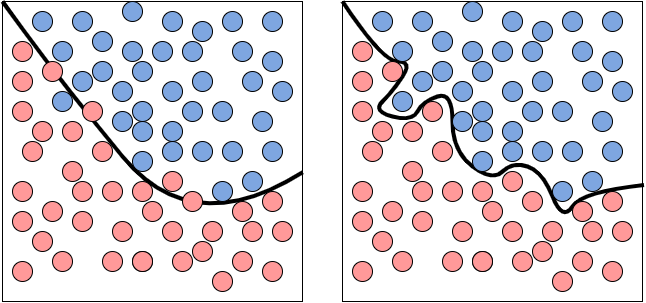
\includegraphics[width= 0.8\linewidth]{Abschlussarbeit_2021/LaTeX/images/tradoff.drawio.png}
\caption{Here is a fictitious seperation problem to see. On the left, all training points were intentionally not memorized in order to be more consistent with new data. On the right, all data points were memorized. This is typical overfitting and can lead to inconsistency with new unseen data.}
\end{figure}

However networks with extremely high capacities interpolate all training data. So they do extreme overfitting i.e. a over adjustment based on the given data, yet their performance is surprisingly good, sometimes even better than models that learn without overfitting. This almost seemingly paradoxical phenomenon is to be investigated in this thesis. For this purpose, the double descent risk curve just described is to be analyzed in detail and assumptions for the cause of the behavior are to be made. 


\begin{figure}[!htp]
\centering
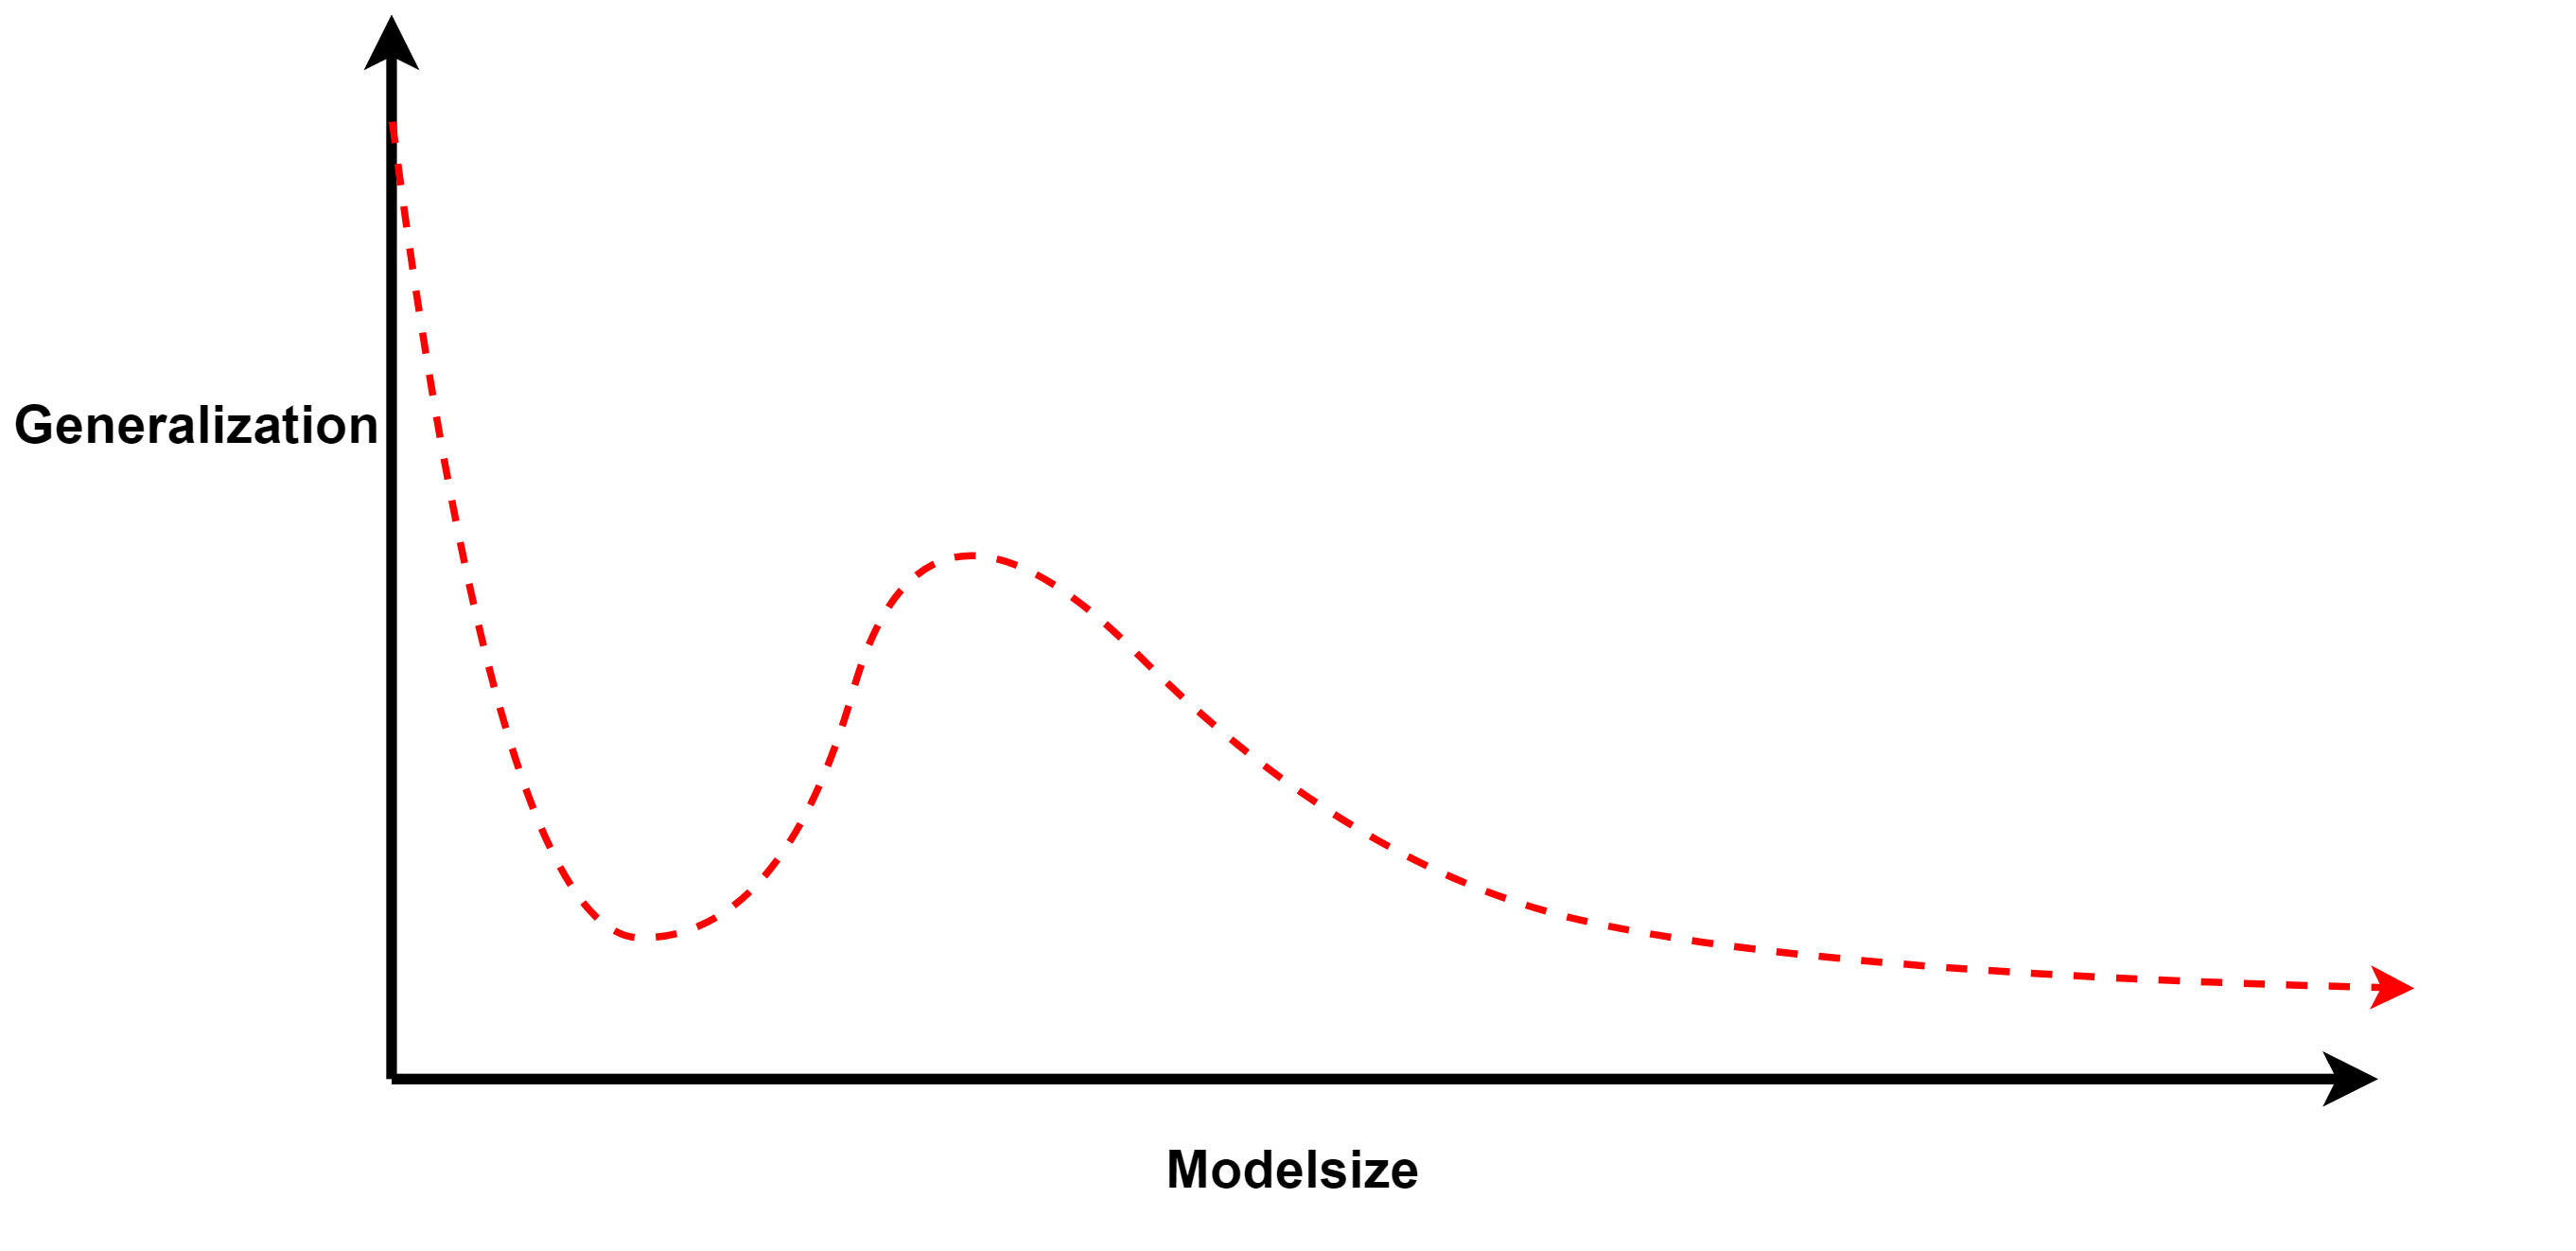
\includegraphics[width= 1\linewidth]{Abschlussarbeit_2021/LaTeX/images/DoubleDescentSkizze.PNG}
\caption{Double descent curve}
\label{double_descent_risk_curve}
\end{figure}

\section{Objective of the Work}

The Thesis is divided into 3 parts. In the first part in chapter 2, the already described Double Descent phenomenon shall be examined more closely. This part is also referred to in the experimental part of the thesis. First the existence of the phenomenon shall be proven and then investigations shall be made, which examine the influence of different parameters on the double descent curve. \\
In chapter 3, the next major part of the thesis, the cause of double descent will be investigated. Particular emphasis will be placed on the possible reasons for the second decrease of the curve. Experiments shall be done, which give information about the changed behavior of larger and larger neural networks. In a detailed analysis possible reasons for the phenomenon will be discussed. \\
The last major part of the work will address the topic of network training, taking into account the phenomenon. Here, among other things, paradoxical effects, which can happen during training, are to be shown. \\
Overall, then, the work focuses on the following questions: Can the shape of the double descent curve be predicted? What influences do certain parameters have on it? What causes the peak of the curve before the second descent? And last but not least the most important question for this thesis: How can the decline of the curve after the peak be explained?




\section{Terms and Definitions}
The following terms are used in the thesis without explanation. 

\begin{itemize}
    \item{\textbf{train loss:}}
    Let $f$ be a learned function of a network and $D = (X_{train},Y_{train})$ be the labeled training data. Thus, the training loss represents a distance between the learned labels and the actual labels using a loss function $l(x,y)$. Thus, the train loss is $l(f(X_{train}),Y_{train})$. If this is zero, then all data points were memorized.
    
    \item{\textbf{test loss:}}
    Same functionality  as the train loss above only that the data points $D = (X_{test},Y_{test})$ are unseen points. Thus, the train loss is $l(f(X_{test}),Y_{test})$.
    
    \item{\textbf{generalization:}}
    Generalization refers to the trained networks ability to adapt properly to new, previously unseen data , drawn from the same distribution as the one used to create the model
    
    \item{\textbf{overfitting:}}
    An over adjustment based on the given data. Focusing too much on training data can lead to poor generalization.
    
    \item{\textbf{underfitting:}}
    An under adjustment based on the given data.
    
    \item{\textbf{test risk:}}
    Also often referred to as empirical risk, describes the risk in predicting unseen data. This risk must be minimized. This is equivalent to minimizing the test loss.
    
    \item{\textbf{SGD:}}
    Stochastic gradient descent (SGD) is an iterative method for optimizing an function. This is achieved by finding minimas in the loss function. Stochasticity is present in it, since the optimization steps are based on random samples only.
    
    \item{\textbf{noise:}}
    Deviation of the data from the actual nominal value. This can happen due to measurement errors or inaccuracies. 
\end{itemize}







% hier weitere Kapitel einbinden
\chapter{Experiments on Double Descent}
\label{experimental_part}

In this chapter, several experiments on generalization of neural networks will be done. The main goal is to demonstrate and explore the double descent risk curve. It shall be discovered, how far the risk curve can be predicted or influenced. The hope is that conclusions regarding the origin of the double descent risk curve can be drawn from the experiments described and conducted in this chapter.\\
What determines the position of the beginning of the second decrease? How can the peak before the second fall of the curve be influenced? Can a point on the curve after the second decrease be found such that the performance is better then after the first decrease of the curve?  It will also be shown that double descent is independent of the minimization algorithm and the data set.

\section{Experimental Setup}

In order to detect or explore double descent, we need a network in which the number of parameters can be increased step by step. A simple method, even if it may not produce the best generalization, would be a network with a hidden layer, i.e. $L = 1$. This hidden layer contains a variable number of neurons $H$. If more parameters are needed, $H$ can be increased. A similar setup was also used in the paper Reconciling modern machine-learning practice and the classical bias–variance trade-off by Mikhail Belkin \cite{belkin}. The neurons in the hidden layer should have connections to all input neurons and all output neurons. The hidden layer is therefore a dens layer. As activation function of the neurons in the hidden layer the  rectified linear activation function or $ReLU$ shall be used. With,
$$
ReLU(x) := \rho(x) = max(0,x)
$$
For almost all experiments, we will use the MNIST dataset, which consists of $60000$ training data and $10000$ Test data \cite{wikipedia_Mnist-Datenbank}. An element from the MNIST set is a greyscale image of a $28 \times 28$ pixel large image, which shows a handwritten number between 0 and 9. The input layer $x$ must therefore have a size of $28 \cdot 28 = 784$. For each pixel one neuron. The training set is normalized before training, so the neurons take a value between $0$ and $1$ as an input depending on the intensity of the represented pixel. The output layer, on the other hand, must have a size of 10 neurons, since we train the model to distinguish between 10 different classes. The activation function for the output layer should be the softmax function $\sigma$, which is given by,
$$
\sigma : \mathbb{R}^{10} \xrightarrow{} [0,1]^{10} \text{ with } \sigma(z)_i = \frac{e^{z_i}}{\sum_{j = 1}^{10}e^{z_j}}.
$$

\begin{figure}
\centering
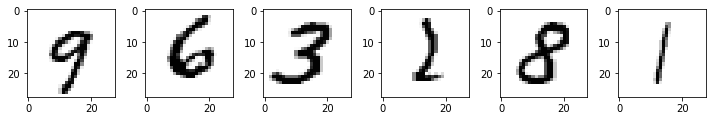
\includegraphics[width= 1\linewidth]{Abschlussarbeit_2021/LaTeX/images/MNIST.png}
\caption{ Six examples of the Trainingset of MNIST}
\end{figure}

The output value of the function is then an array of length 10, where the i-th entry contains the probability for class i. Let $y$ be the output of the output layer so the classification of the input is given by $y_i = \arg\max_{i \in \{1, \cdots,10\}}(y)$. \\
The model $M$ which is used in the following experiments can thus be represented mathematically by,
\begin{equation}
    M(x) = \arg\max(\sigma_0, \cdots \sigma_9) \\
    \text{ with } \sigma_k = [\sum_{i = 1}^H w^{(2)}_{i,k} \cdot \rho(\sum_{j=1}^{784}w^{(1)}_{j,i}\cdot x_j) + b^{(1)}_i] + b^{(2)}_k
    \label{model equation}
\end{equation}

Where $w^{(1)} \in \mathbb{R}^{784 \times H}$ is the weight matrix between the input layer and the hidden layer and $w^{(2)} \in \mathbb{R}^{H \times 10}$ is the weight matrix between the hidden layer and the output layer. The bias vector for the hidden layer is $b^{(1)}$. $b^{(2)}$ is the bias vector from the output layer. All weights in the weight matrices and all biases in the layers should be allowed to change through the optimization process. The number of parameters that can be trained depends only on $H$, because input and output layer always have the same size. The amount of trainable Parameters $P$ is therefore given by,
$$
P(H) = (784+1)\cdot H + (H+1) \cdot 10
$$
As a loss-function, category crossentropy should be used, as it is usual for classification problems. Which is given by,
\begin{equation}
    L(x) =  - \sum_{i = 0}^{9} y_i^* \cdot \log y_i
    \label{scc_eq}
\end{equation}
where $y = [y_0,y_1 \cdots, y_9] = M(x)$ is the output of the model in equation 2.1, whereas $y^* =[y^*_0,y^*_1 \cdots, y^*_9]$ is the target value i.e how the model should react. For example if the label of a point $x$ is $4$, $y^*$ would be $[0,0,0,0,1,0,0,0,0,0]$. \\
To minimize the loss function $L(x)$ stochastic gradient descent (SGD) is used. This is done by updating the weights and biases into the direction of the approximated gradient.
$$
w_{i,j}^{(n+1)} := w_{i,j}^{(n)}  - \eta \frac{\delta L}{\delta w_{i,j}}
$$
%%TODO: OPTIMIZE Formula. 
%%%%%%%%%%%%%%%%%%%%%%%%%%%
%%%%%%%%%%%%%%%%%%%%%%%
%%TODO!!!!!!!!!!!!!!!!!!!!!!

where $w_{i,j}^{(n)}$ is the weight matrix at $i,j$ at iteration $n$. The same rule holds for the biases. $\eta$ is the learning rate or the stepsize. In the following experiments a learning rate $\eta = 0.05$ will be used. By minimizing the loss function the model performs better and better on training data. \\
In the introduction, the question was asked why, despite a loss function that assumes extremely low values in the training data, a network still performs very well. That is why an extremely small training loss is always achieved during training from a certain model size.



\newpage

\section{Experiments}

Before more complex experiments are performed, the existence of the double descent curve described in Beklin's paper should be empirically proven. For this purpose a model $M$ from equation \ref{model equation} is taken. $M$ is thereby supposed to have $1 \leq H \leq 80$ neurons. Thus, a total of 80 training sessions are run. The training and test loss is measured at each iteration of $H$. The training process is stopped when either $200$ epochs have been reached or a test-loss below $0.001$ has been reached. $M$ was trained on a subset of MNIST with $20000$ Samples. It could be argued that stopping earlier for large networks contributes to the second drop of the curve, since this way overfitting is no longer done. However, this is not the case. Stopping at a certain test loss is only done to save time. Figure \ref{fig:epochs_double_descent} shows double descent curves, where independent of the model size always the same number of epochs was run through. This curve looks very similar to the one in Figure \ref{double_descent_vanilla}.

\begin{figure}[!htp]
\centering
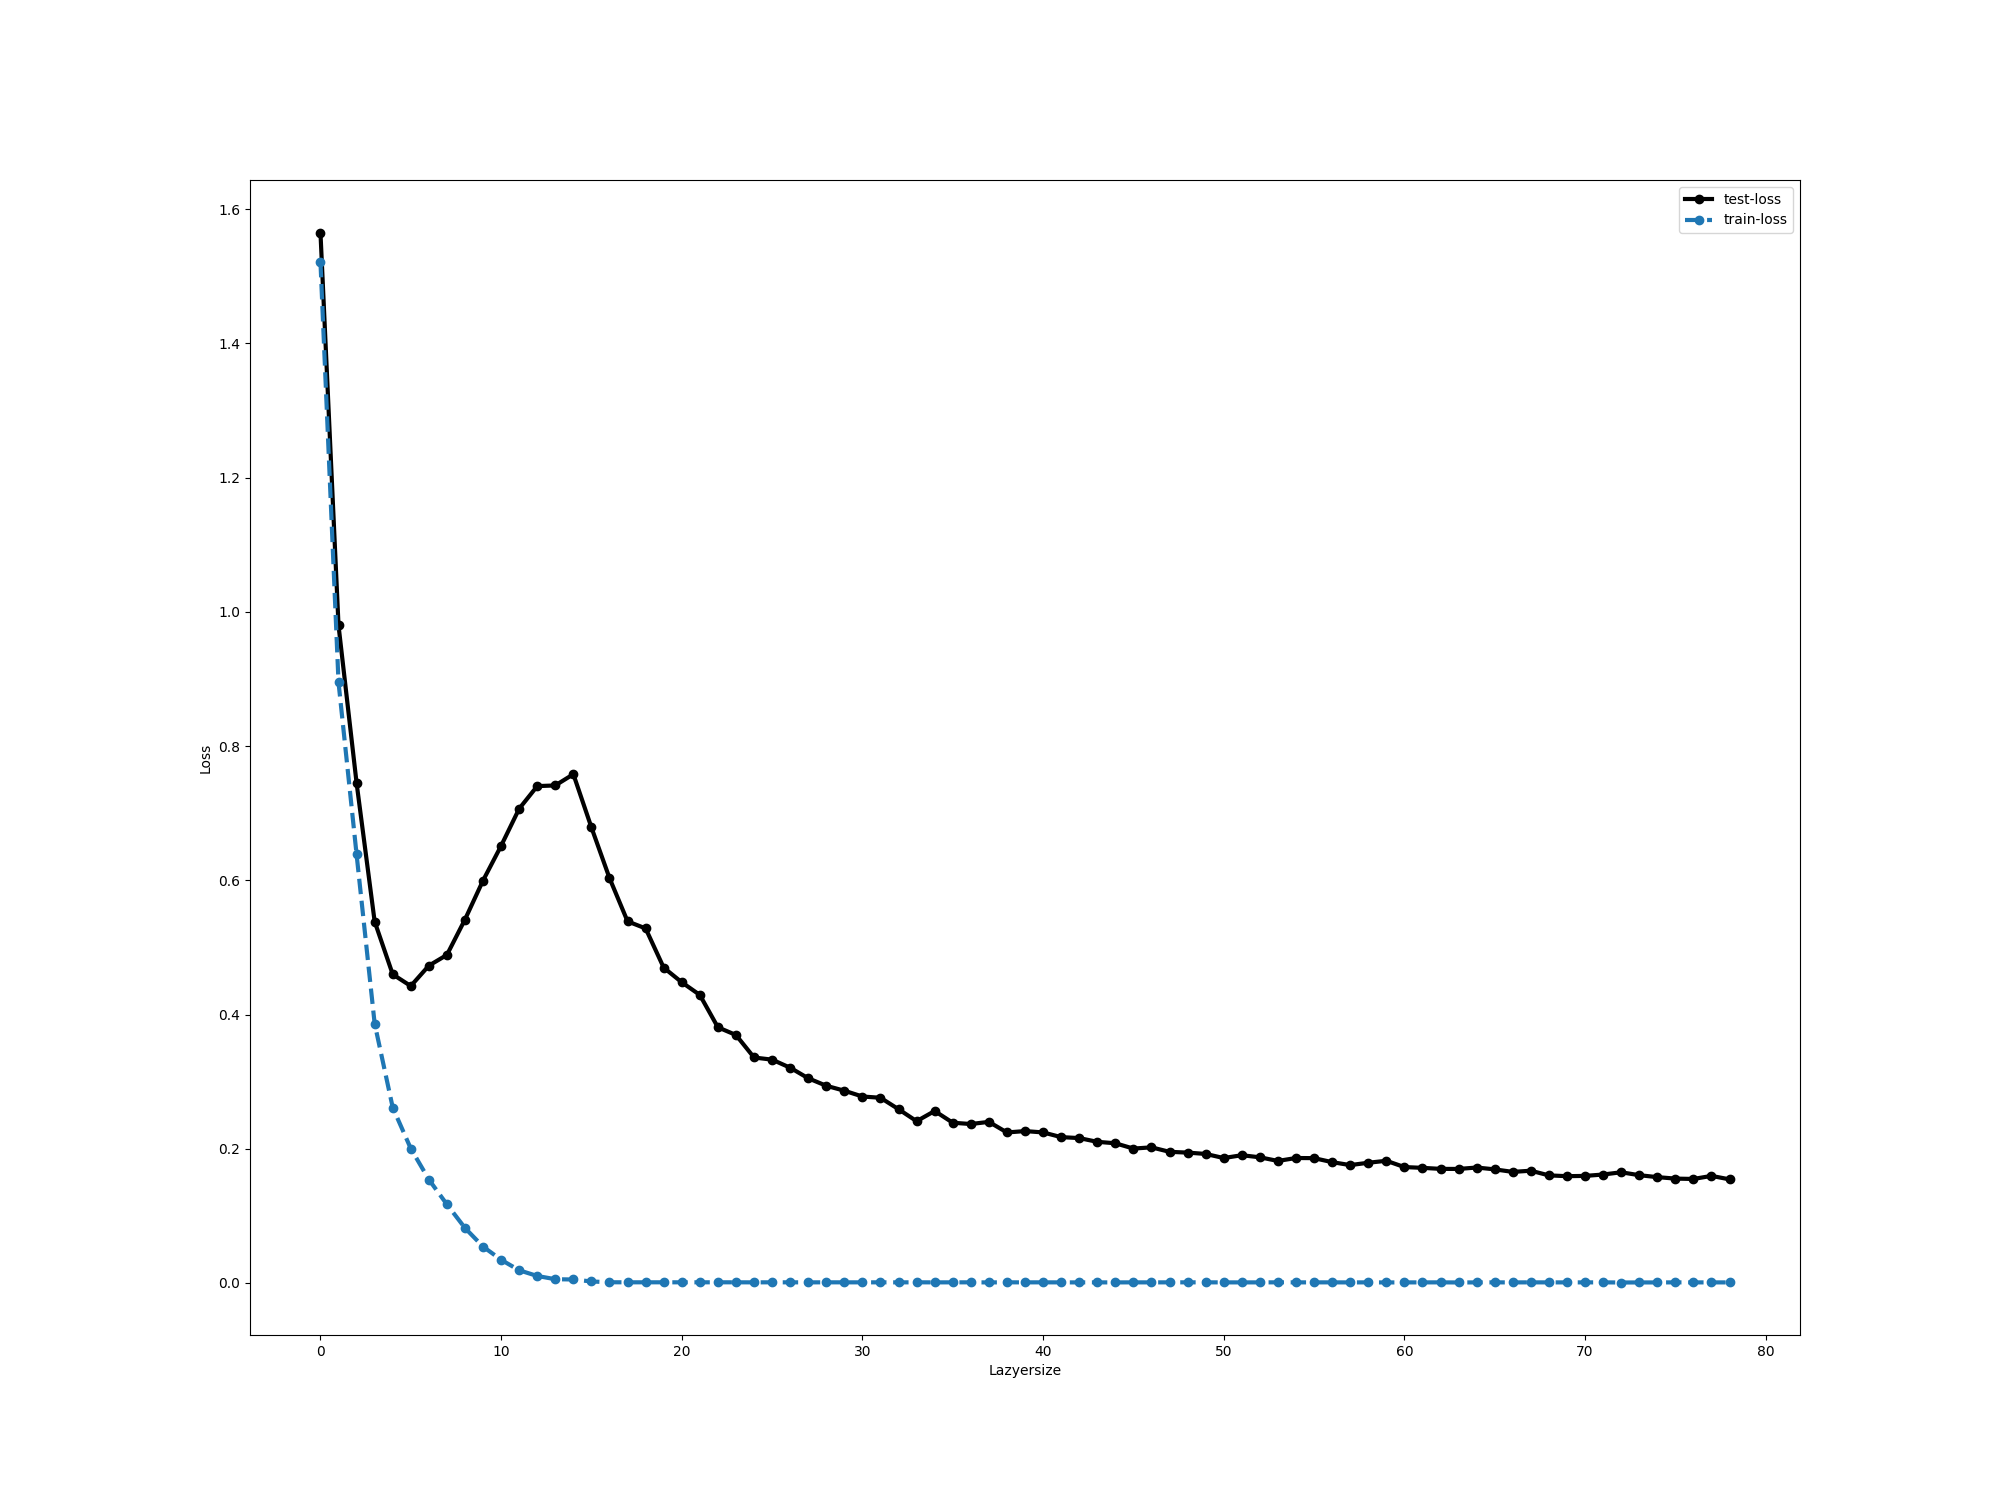
\includegraphics[width= 1\linewidth]{Abschlussarbeit_2021/LaTeX/images/double_sgd.png}
\caption{Train-loss and test-loss averaged over 10 runs}
\label{double_descent_vanilla}
\end{figure}

In Figure \ref{double_descent_vanilla}, two important observations can be made. The first one is that the performance of $M$ is better from a certain number of neurons ($H = 21$) than before the peak. Even if the training was not optimal up to the local maximum, because the model was overfitted with 200 epochs, the generalization is extremely good at $H = 80$. Here a test accuracy of $97\%$ was achieved. 
the second observation that can be made concerns the position of the peak. This can be observed at $H = 16$. The test loss, on the other hand, is zero the first time from $H = 16$. The peak is called \textit{"interpolation threshold"} by Belkin \cite{belkin}. The reason for this is that the data can be interpolated from this point because the model has sufficient capacity. The region to the left of the interpolation threshold is called \textit{"underparameterized regime"} and the region to the right of the interpolation threshold is called \textit{"overparameterized regime"}. overparameterized and underparameterized respectively, because there are more than enough or not enough parameters to learn the training data perfectly.\\
In the further part of the section the effect on the shape of the curve will be tested by changing different attributes. How does the curve behave when changing the sample size? What influence does the number of epochs have? And what happens when the labels are replaced with noise during training?

\subsection{The influence of data quantity}

If the data quantity is reduced or increased, the peak at the interpolation threshold shifts to the left or to the right, respectively. 
This means the model can reach a zero percent test loss faster if the amount of data is smaller. This is a very predictable and logical finding. It is interesting, however, that the statement \textit{"more data is always better"} is not that clear to observe. On the one hand, a model $M_{H=80}$\footnote{Model with $80$ neurons in the hidden layer} trained with 5000 samples and 80 neurons can perform better than a smaller model $M_{H \leq 20}$ with up to 20 neurons trained with 20000 samples.
For large and small $H$, the performance is clearly better when more data was used to train. However, there is a range $(10 \leq H \leq 22)$ where the order of generalization is not entirely clear.\\
This will be discussed in more detail in chapter \ref{train_dd}. For small $H$ with $5 \leq H \leq 10$ and large $23 \leq H $, it is clear that more data improves the generalization. The peaks at the interpolation threshold are somewhat broader for larger data sets.  

\begin{figure}[!htp]
\centering
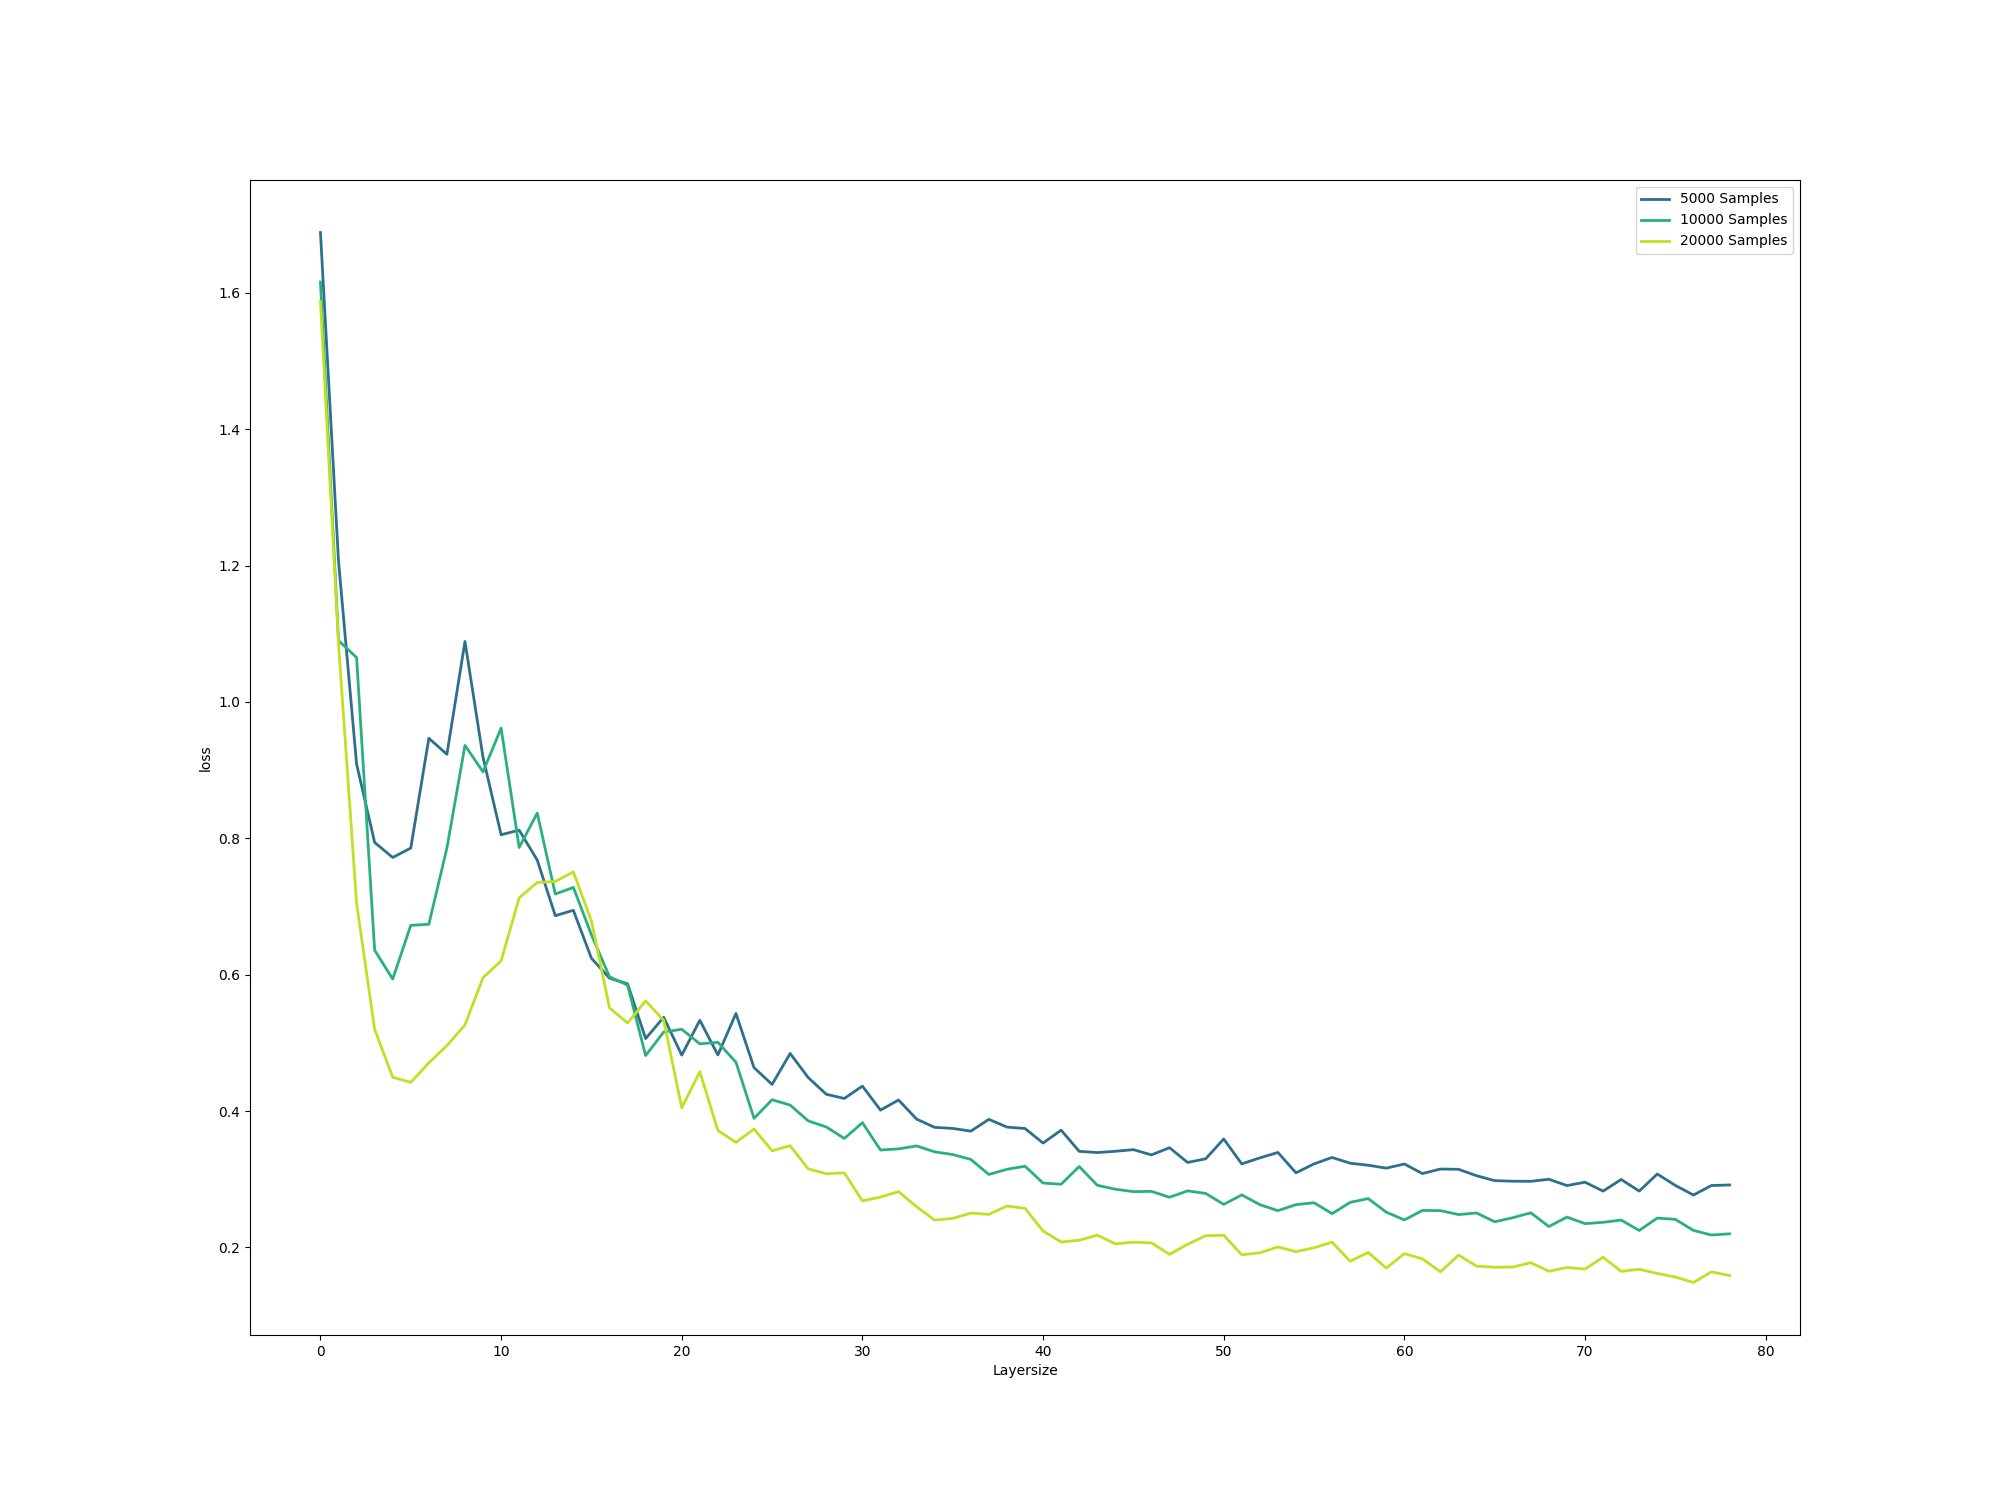
\includegraphics[width= 1\linewidth]{Abschlussarbeit_2021/LaTeX/images/diff_samplesizes.png}
\caption{test-loss averaged over 2 runs. The experiment was performed with 3 different sized subsets of MNIST.}
\label{fig:sample_size_double_descent}
\end{figure}



\subsection{The influence of epochs}


It is known that overfitting can occur when training neural networks by running through too many epochs. The model then can perform worse on unseen data.   



\begin{figure}[!htp]
\centering
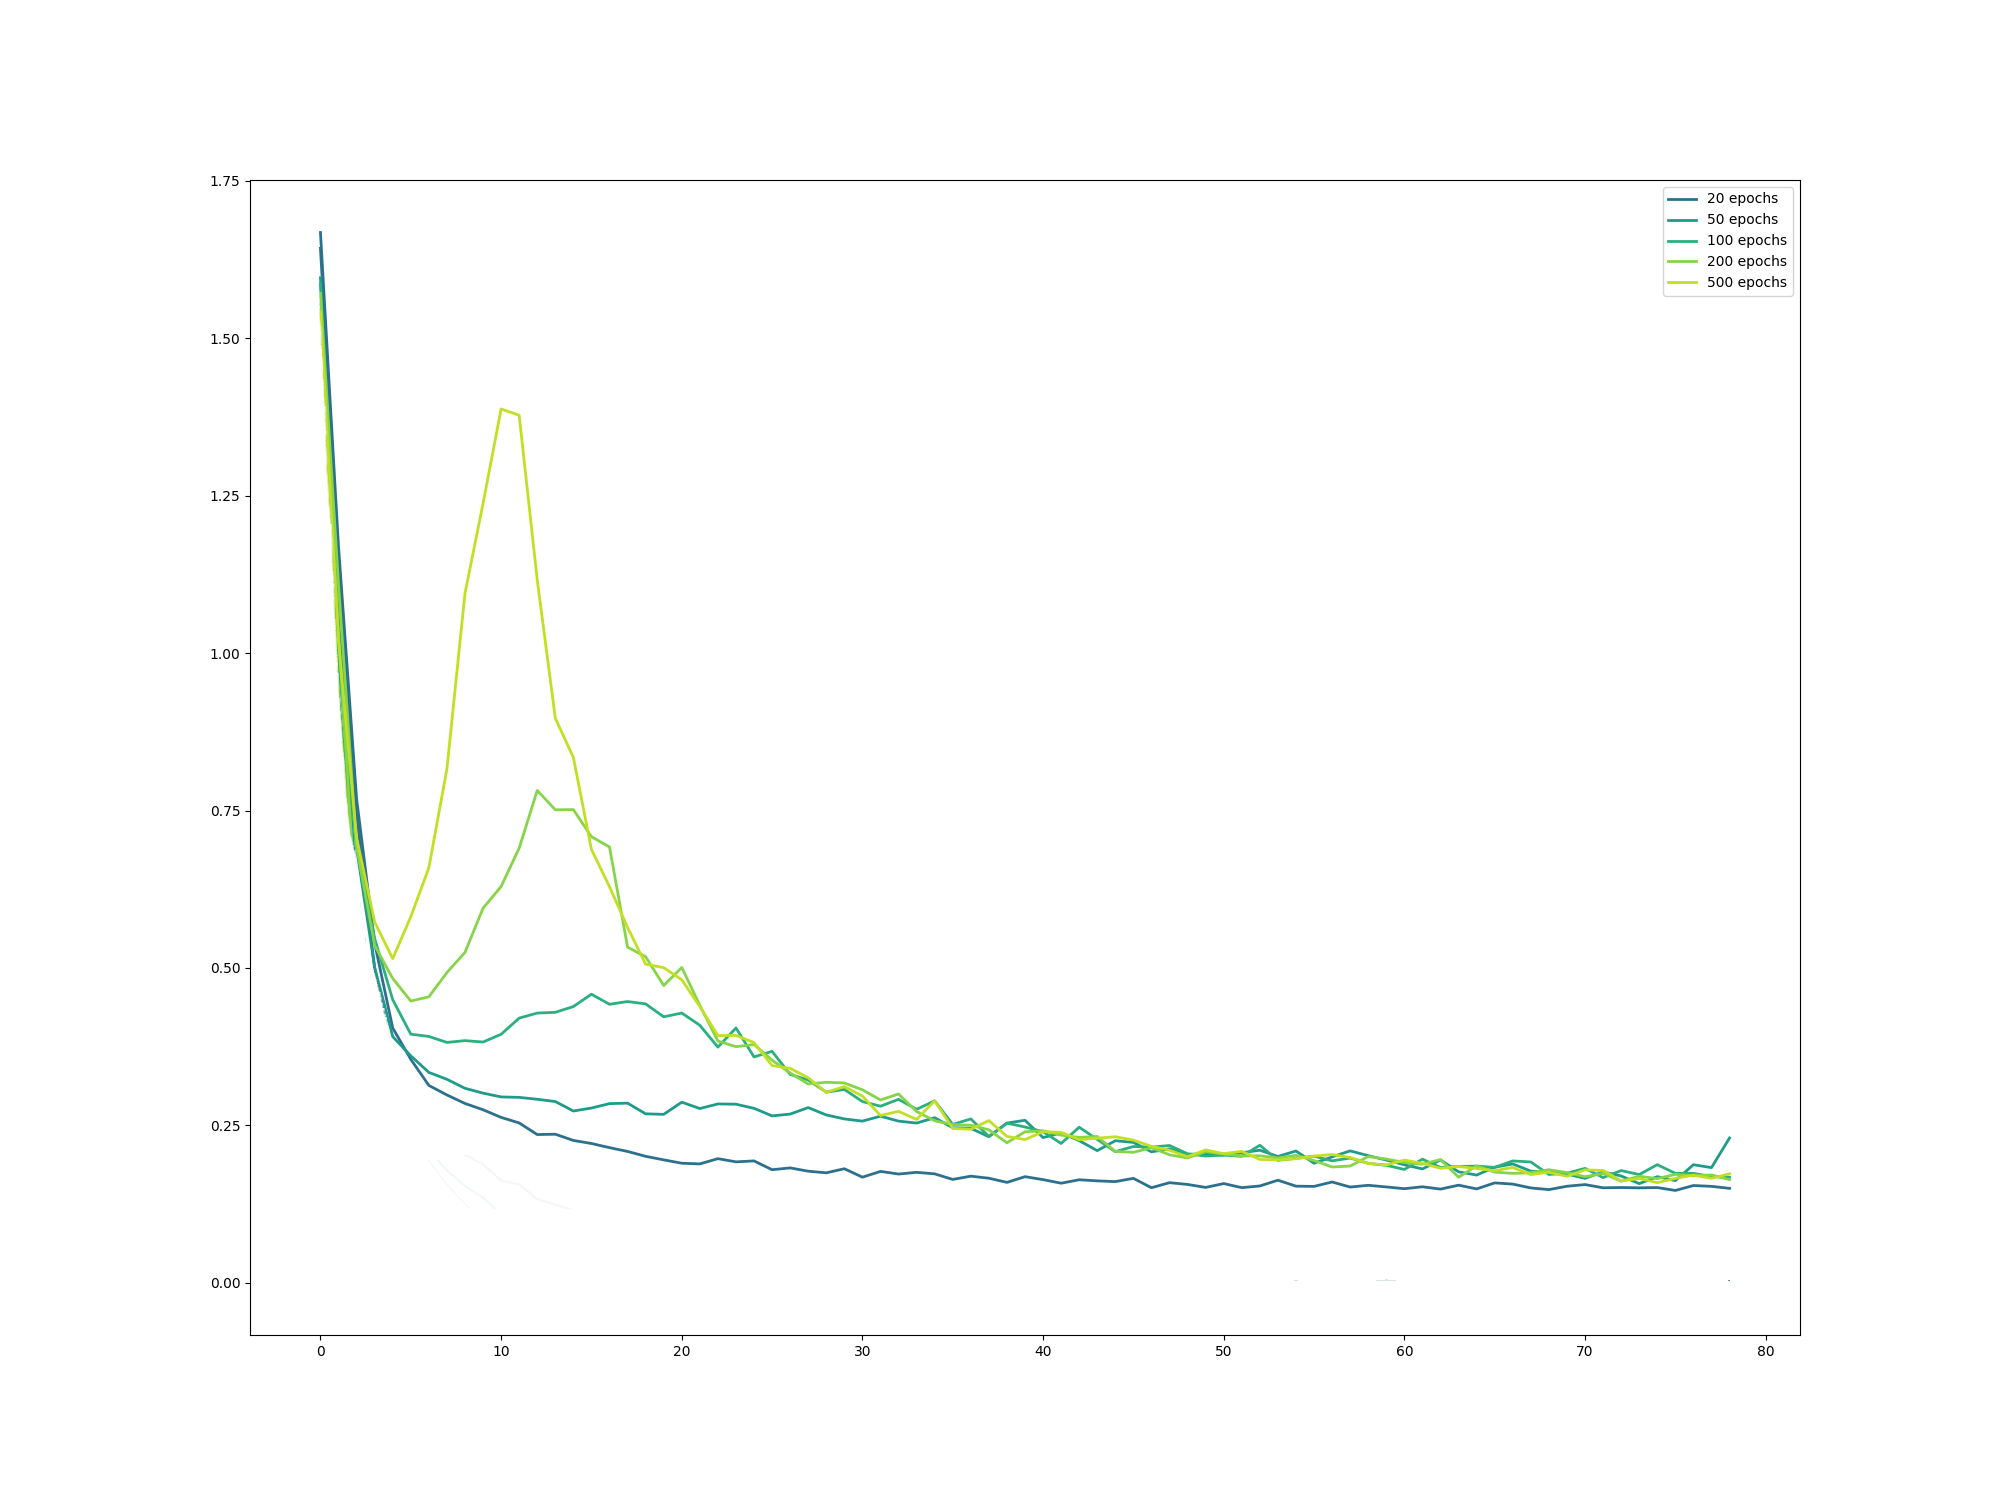
\includegraphics[width= 1\linewidth]{Abschlussarbeit_2021/LaTeX/images/many_epochs.png}
\caption{Test-loss depending on the amount of epochs averaged over 4 runs}
\label{fig:epochs_double_descent}
\end{figure}


Figure \ref{fig:sample_size_double_descent} clearly shows that the number of epochs has a large influence on the peak at the interpolation threshold. The more epochs are passed through, the higher is the peak. 
Double descent can even be completely omitted with the selected architecture if training was carried out with only a few epochs. In addition, the interpolation threshold moves further and further to the left as the number of epochs increases. The perfect interpolation of the data happens already with smaller $H$. This finding is logical, because at certain $H$ after a few epochs no minimum with zero train loss was found, which interpolates the data perfectly. If one would run through more epochs, however, the said minimum can be found.
As mentioned above, the training was not ended prematurely when a certain training loss was reached. The test loss is very similar for all epoch numbers for large $H$. This is also an interesting finding.




\subsection{The influence of noise}

As has already been observed, the train-loss after the interpolation threshold is zero. This means that the data is perfectly memorized. The MNIST data set possesses little noise. Even though some numbers are drawn inaccurately, the label is always appropriate to the image. However, in many more complex applications, there is often a lot of noise in data sets. Labels are sometimes not fitting to the respective data point (label noise). Measured values could also become inaccurate due to different environmental influences. In such cases, is it necessarily wanted that the model learns all its training data perfectly by memory? As will be shown later, noise causes a high variance in the set of possible learned function. This means that if the network is trained more often, the resulting learned functions will be more different from each other. To memorize this noise, the model also needs significantly more capacity. In the case of MNIST, the model could remember that at label $7$ the pixel $(x,y)$ is active. Due to label noise, it can happen that an actual image of a $6$ is labeled as $7$. So the simple constrain $7 \	\Longrightarrow (x,y) > 0.8$ is not sufficient, and the model must find more complex structures to get the label noise under control.\\
The effect can be observed in Figure \ref{fig:Label_noise_on_double_descent}. With increased label noise, the peak at the interpolation threshold is seen much later. In addition, the test loss value is also significantly higher there. However, it can also be assumed that for large $H$ and with not too high label noise, the model performs better in the overparameterized region than in the underparameterized region, since the curves are still decreasing after $H = 80$. For certain $H$ it can even be seen that paradoxically more noise leads to better generalization. This point will be taken up again in \ref{less_noise_can_hurt}. 


\begin{figure}[!htp]
\centering
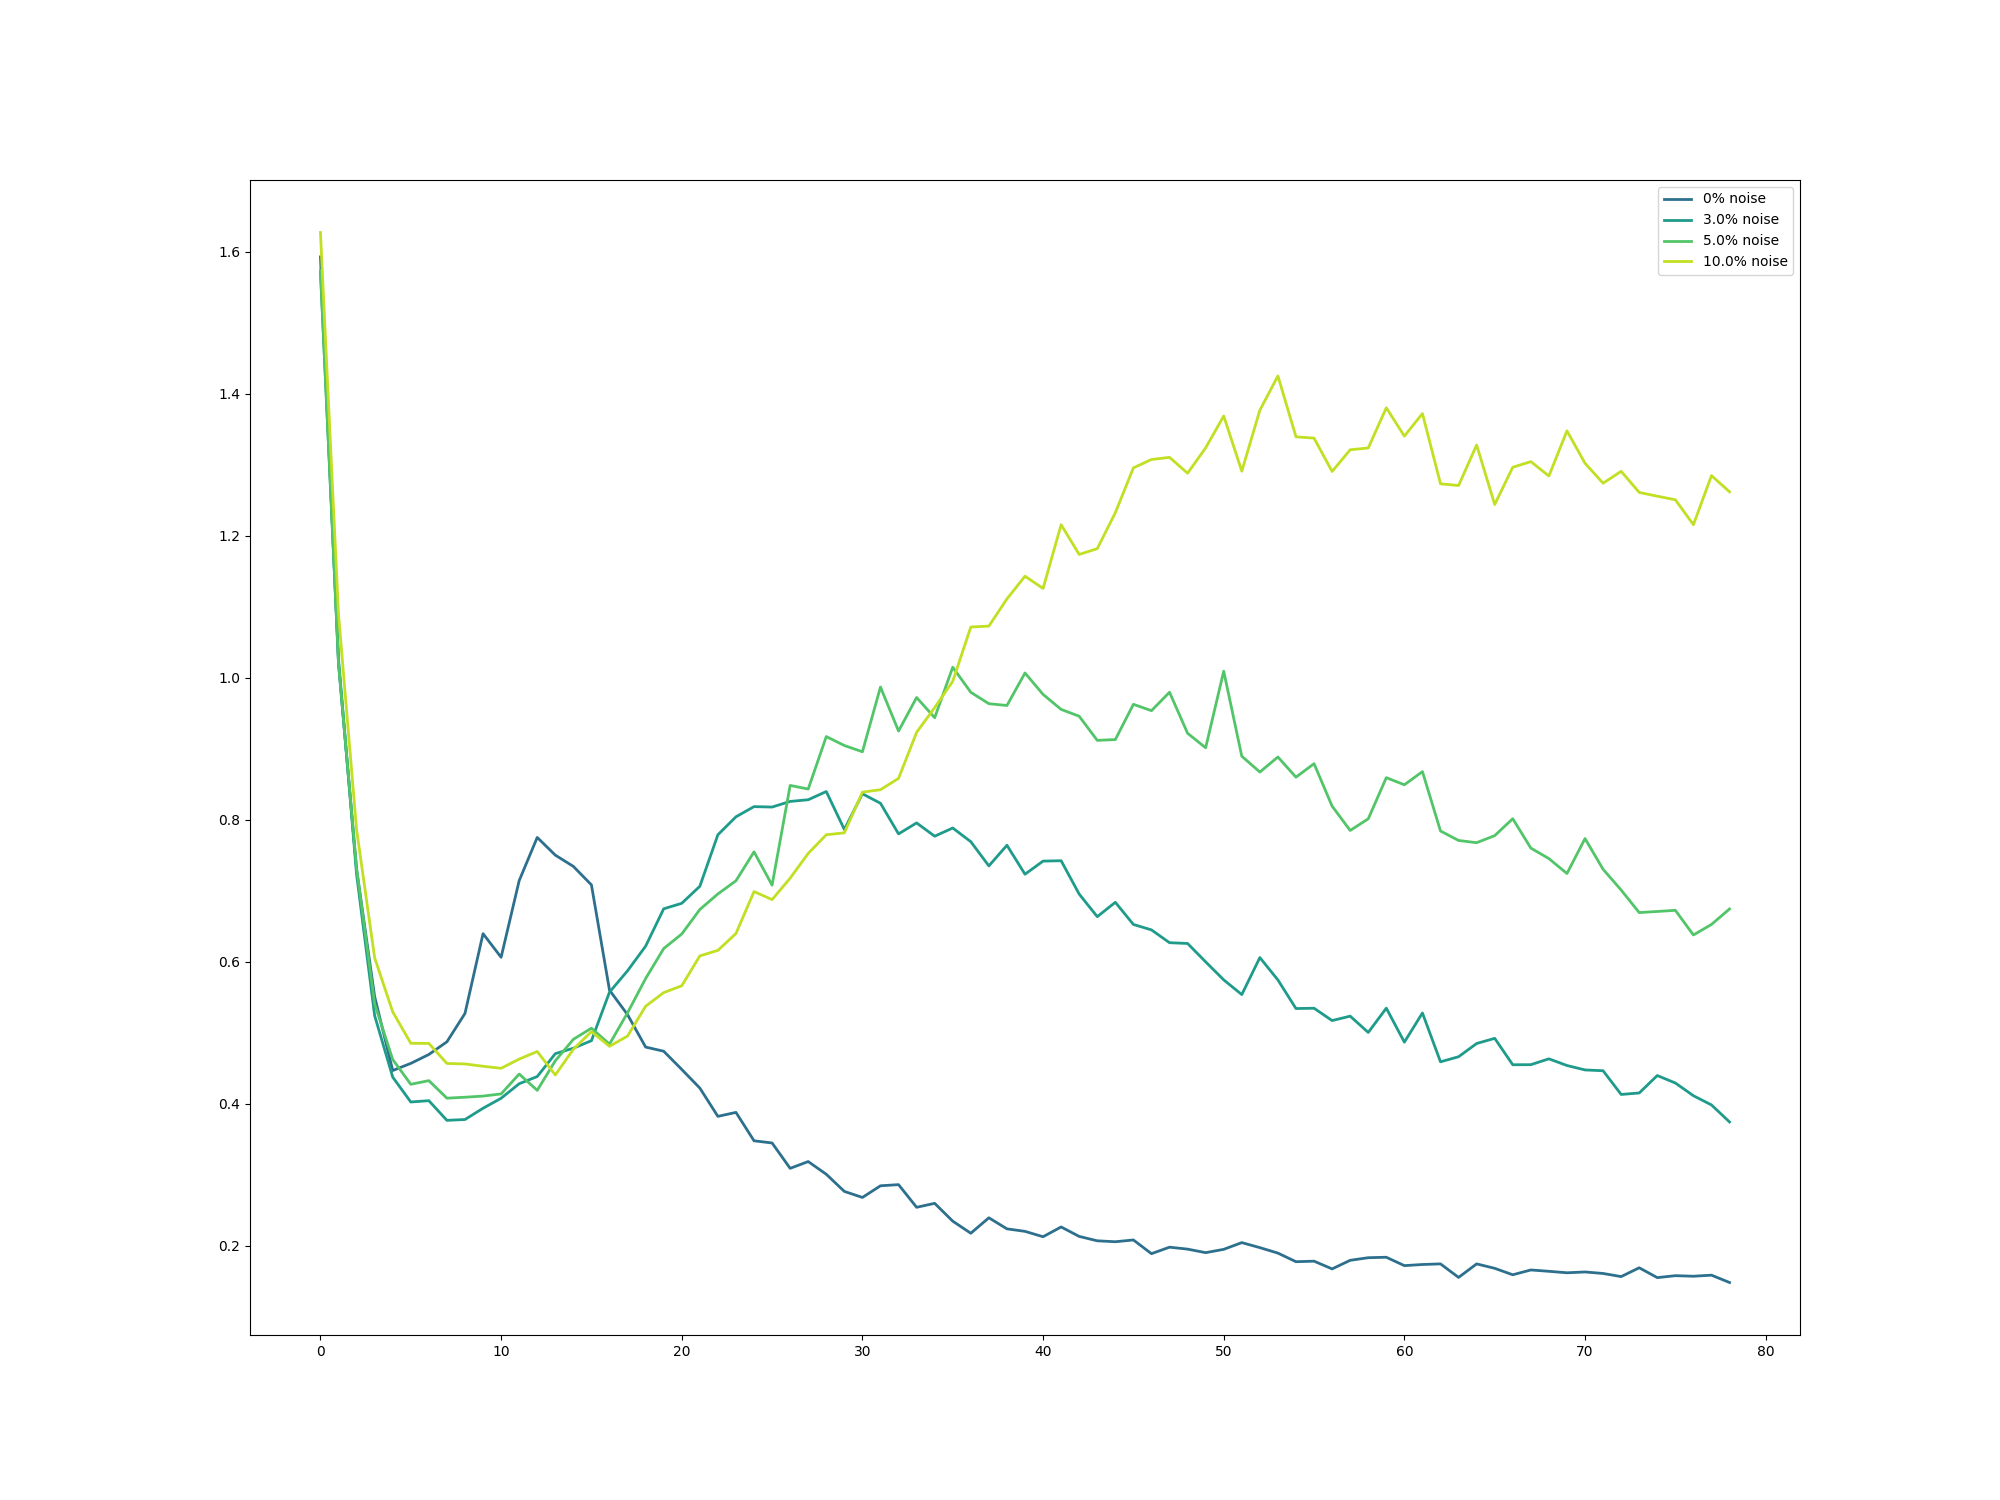
\includegraphics[width= 1\linewidth]{Abschlussarbeit_2021/LaTeX/images/many_curves_less_noise.png}
\caption{Test-loss with different label noise averaged over 4 runs. For the experiment noise was added to the labels. This means, that for a certain probability the label was chosen randomly. The probabilities for each curve is given in the legend.}
\label{fig:Label_noise_on_double_descent}
\end{figure}

%%%%%%%%%%%%%%%%%%%%%%%%%%%%%%%%%%%%%%%%%%%
%%%%%%%%%%%%%%%%%%%%%%%%%%%%%%%%%%%%%%%%%%%
%%%%%%%%%%%%%%%%%%%%%%%%%%%%%%%%%%%%%%%%%%%

\newpage
\section{Double Descent with Optimizer and Data sets}

In the previous experiments, the models were always trained with stochastic gradient descent (SGD). 
Double descent is not only a phenomenon that occurs when training with SGD. The peak can also be seen when training with the ADAM algorithm.
Figure \ref{fig:double_descent_on_optimizers} shows that the peak at the interpolation threshold can also be clearly observed. 

\begin{figure}[!htp]
\centering
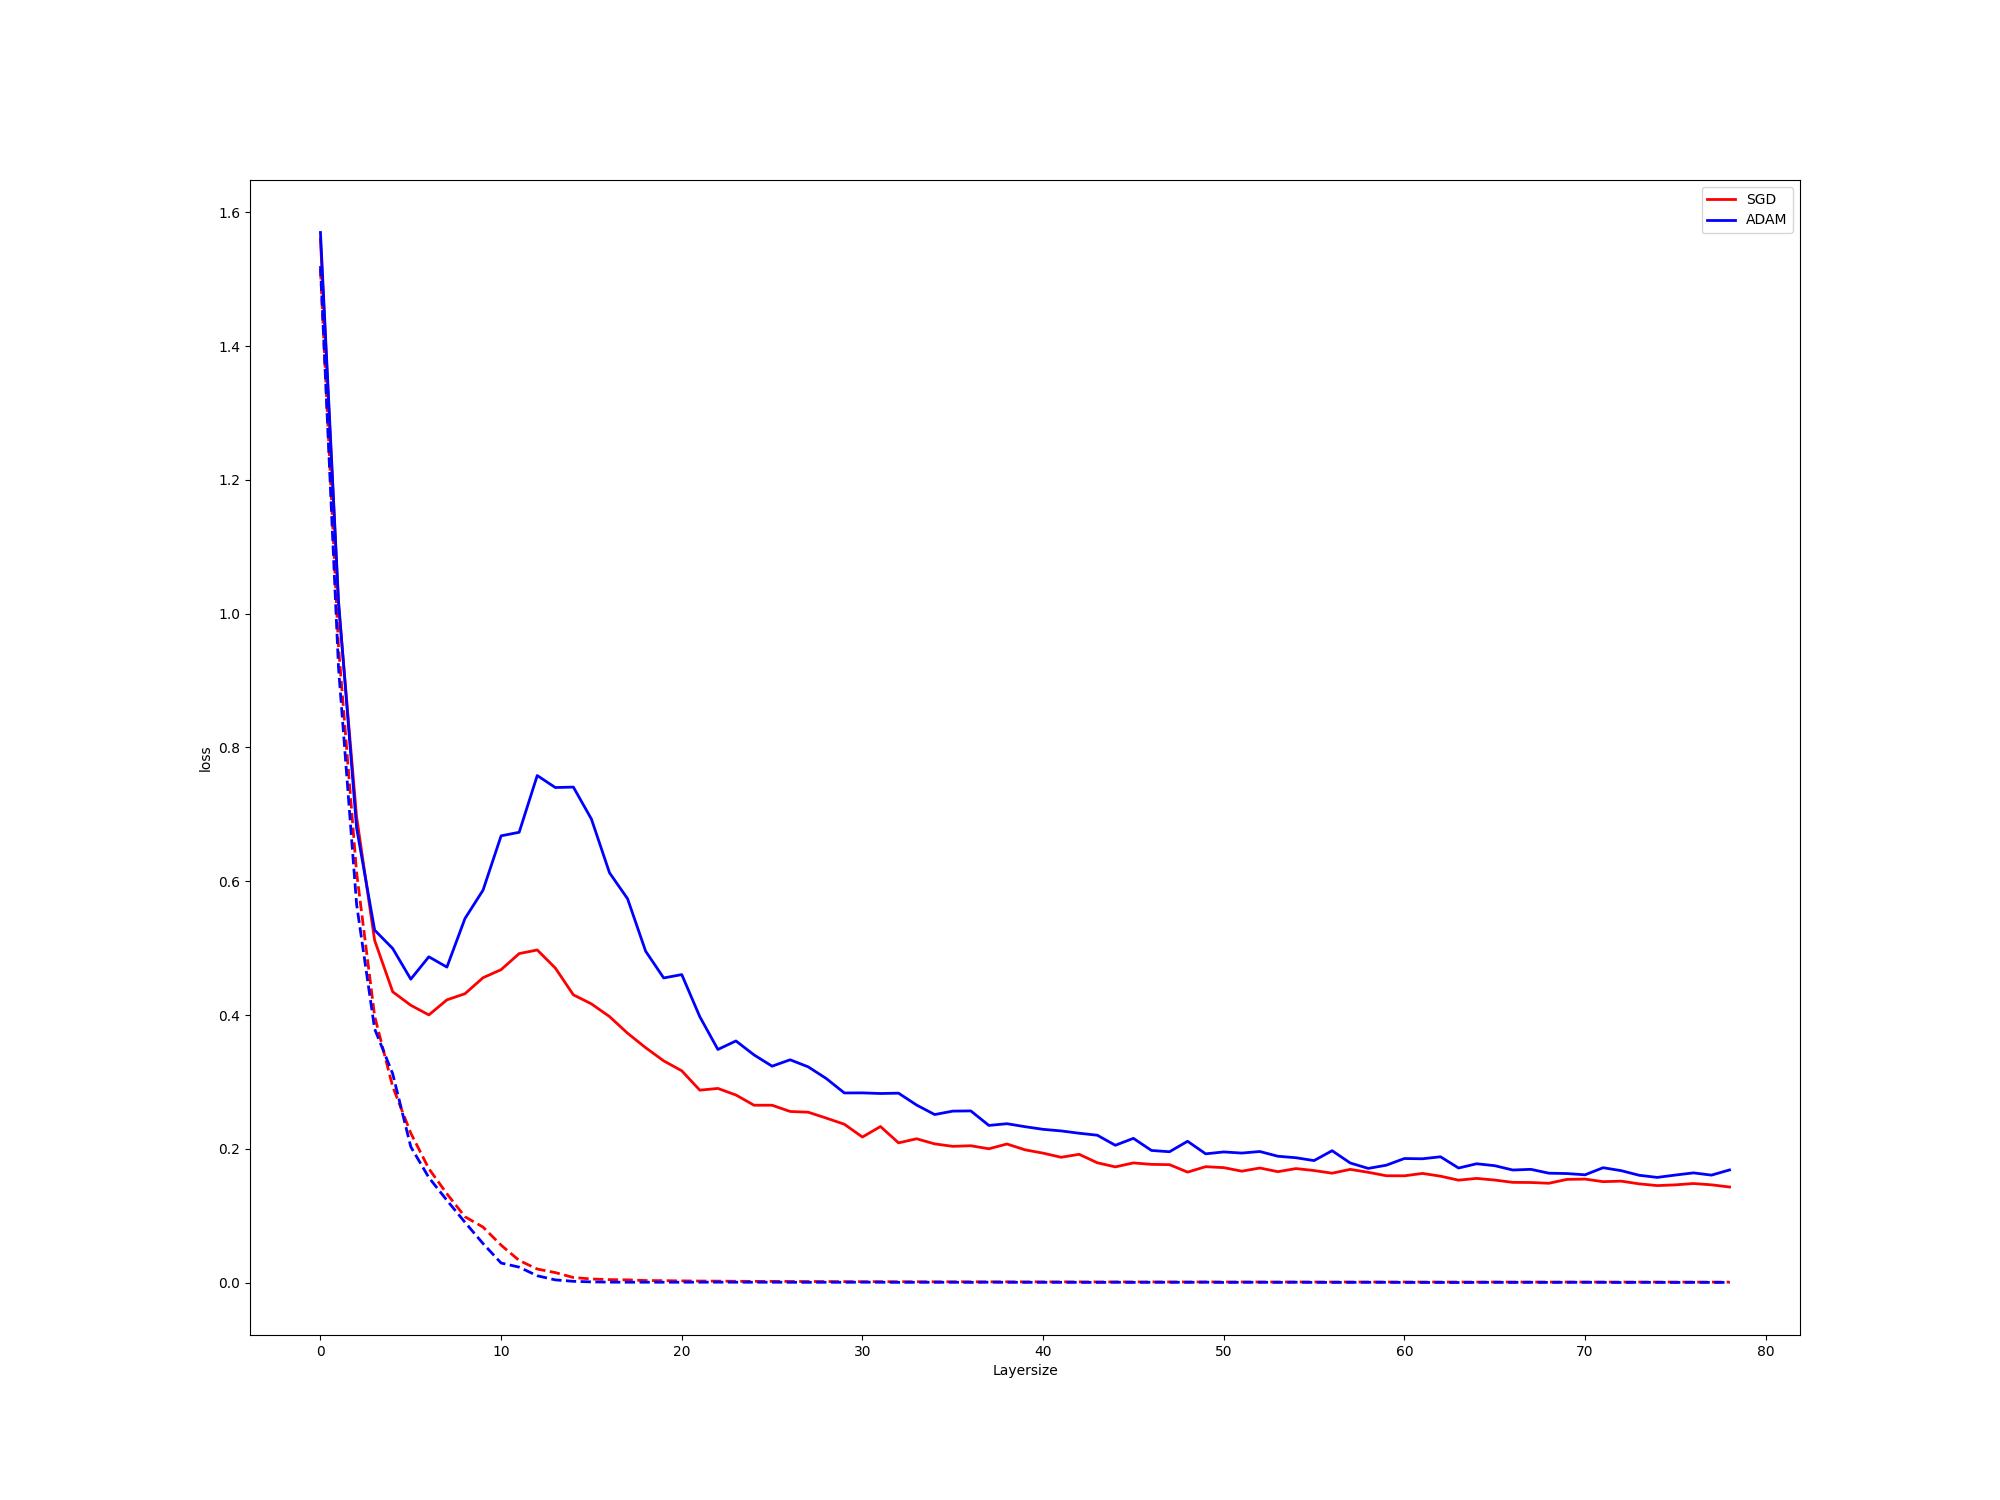
\includegraphics[width= 1\linewidth]{Abschlussarbeit_2021/LaTeX/images/ADAM_vs_SGD.png}
\caption{train and test loss from ADAM and SGD. averaged over 4 runs}
\label{fig:double_descent_on_optimizers}
\end{figure}

One difference between the adam-optimizer and SGD is that the learning rate varies with adam. In SGD this is not the case without instruction. The red curve of the model trained with SGD in \ref{fig:double_descent_on_optimizers} was generated by a learning rate of $\eta = 0.05$. Figure \ref{fig:learning_rates_double_descent} shows that by changing the learning rate $\eta$ the peak of the curve can be changed. Thus, at a higher learning rate, the test loss at the interpolation threshold is significantly higher than at a lower learning rate. If $\eta$ is small enough, it is even possible that no double descent can be seen, unless the model was trained without label noise. The surprisingly high peak, which occurred when using adam, can also be generated with SGD if the learning rate is appropriate. \\
The graph looks similar to the ones in Figure \ref{fig:epochs_double_descent} where the epochs where varied. This might due to the effect, that higher learning rate and processing more epochs have a similar effect on weight change. We will deepen this in Chapter \ref{possible_explanations}. 

\begin{figure}[!htp]
\centering
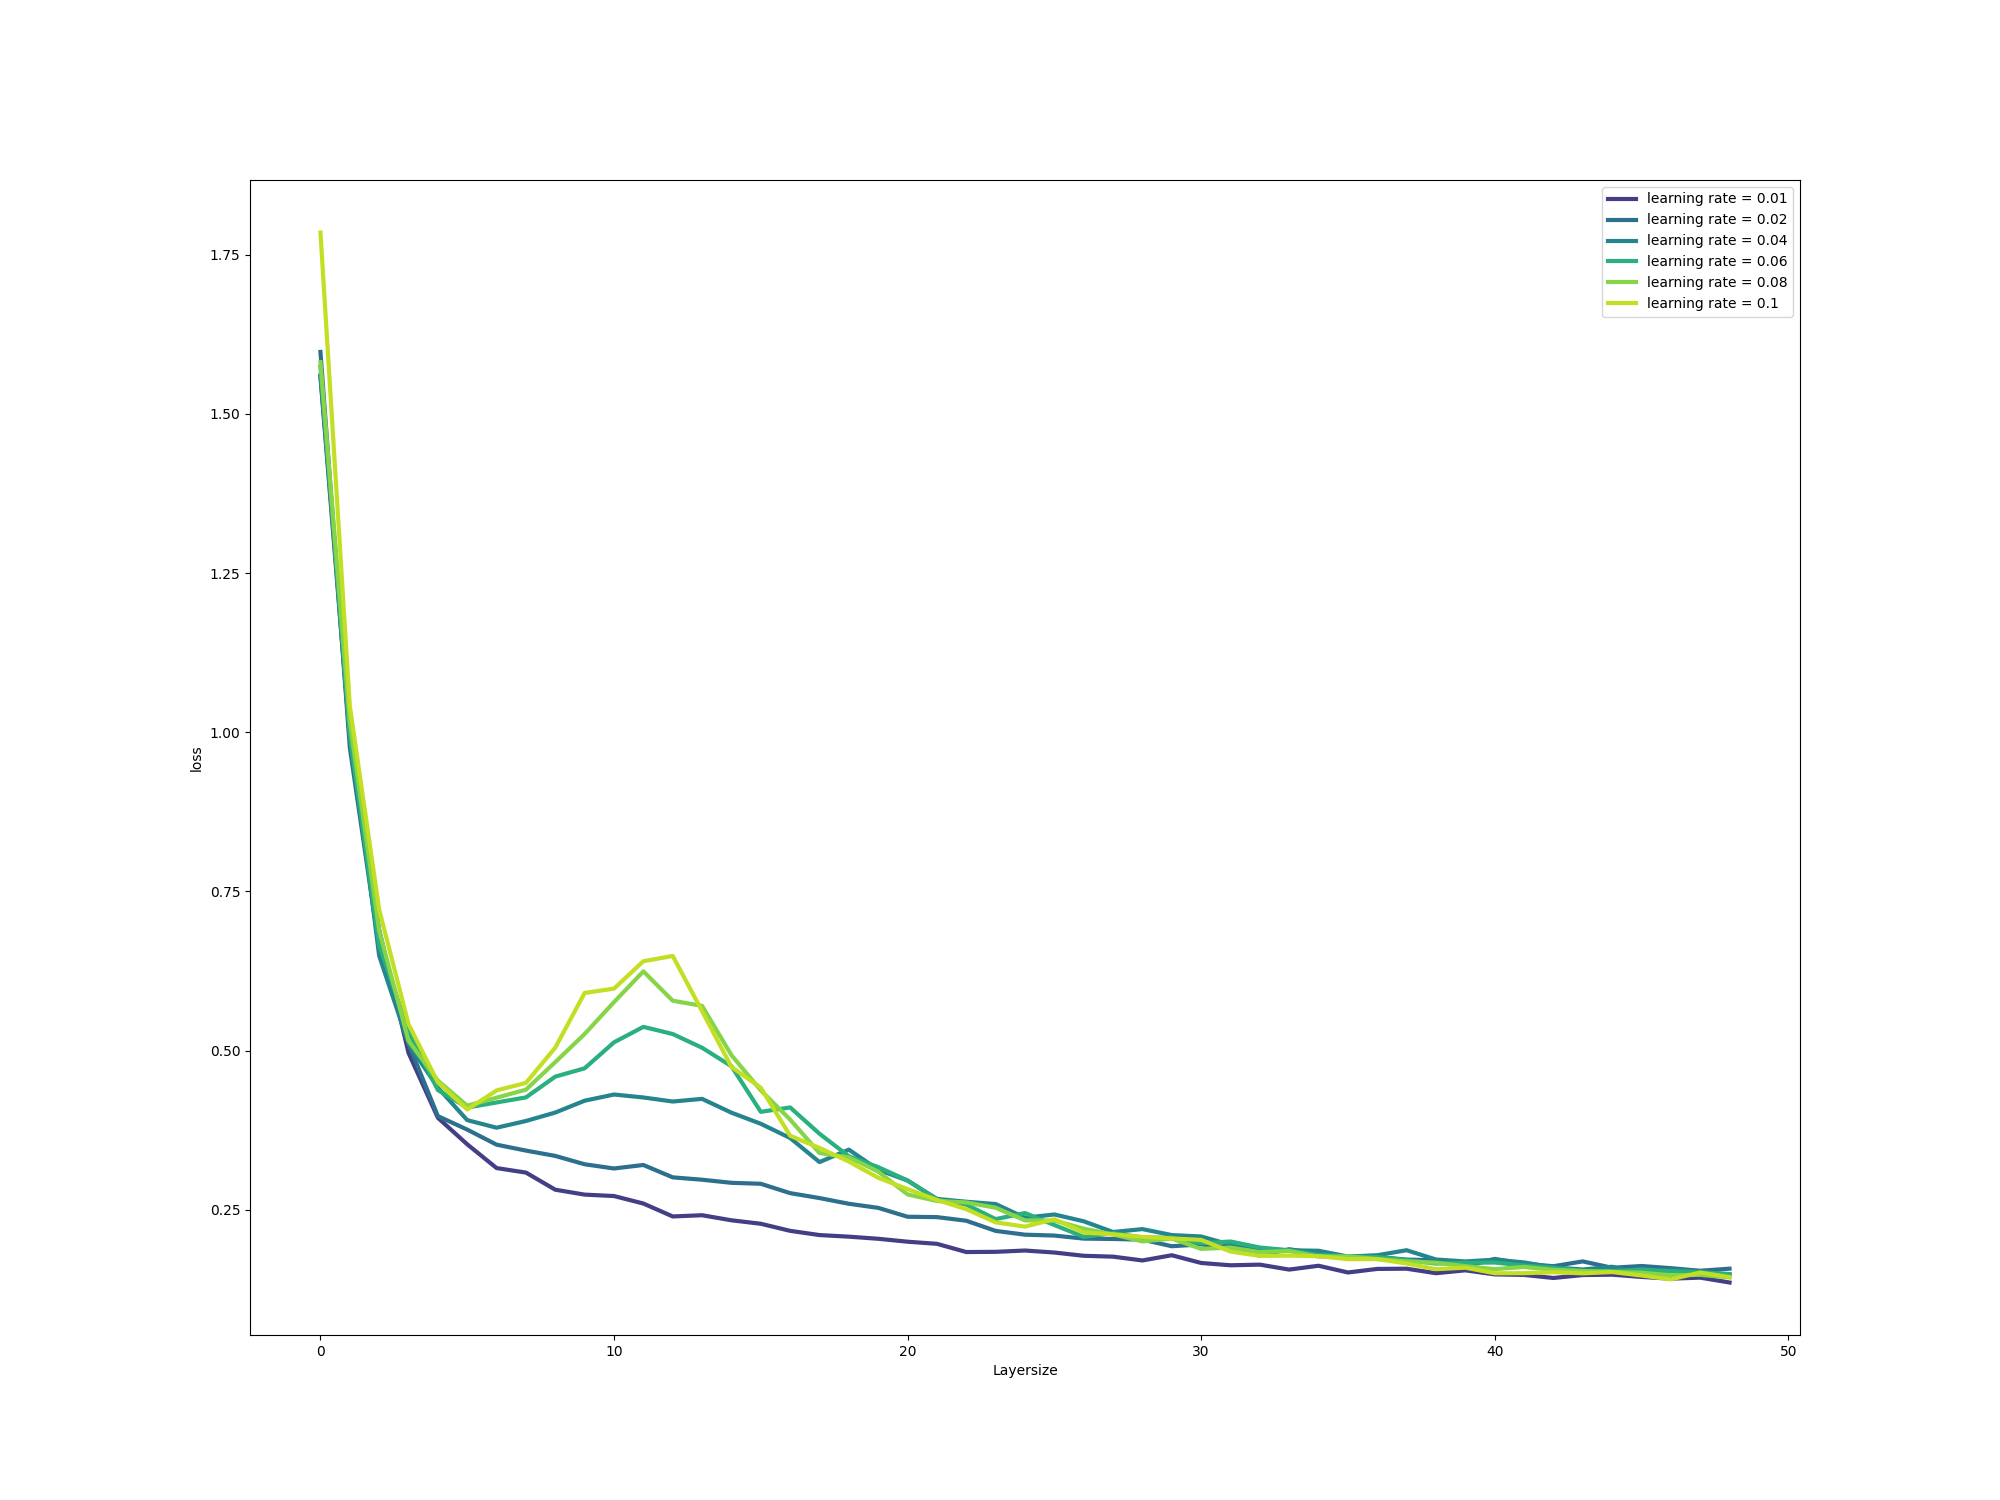
\includegraphics[width= 1\linewidth]{Abschlussarbeit_2021/LaTeX/images/different_learningrates.png}
\caption{test-loss with different learning rates. The curves where averaged over 6 runs. A higher learning rate $\eta$ results in a higher peak at the interpolation threshold}
\label{fig:learning_rates_double_descent}
\end{figure}

\subsubsection{Double descent with different architecture}
To demonstrate that double descent can occur with other loss functions, data sets, and network architectures, a regression problem has been treated in Figure \ref{fig:double_descent_wine} Here the loss function mean squared error (MSE) was used, which is given by,

\begin{equation}
    MSE = \frac{1}{n}\sum_{i=1}^{n}(f(x_i) - y_i)^2
    \label{mse_eq}
\end{equation}

Where $x_i \in X$ is a training point, $y_i$ the corresponding label and $f(x)$ is the function which is represented by the model. This time two fully connected hidden layers were used. The layer size in Figure \ref{fig:double_descent_wine} indicates the size of both hidden layers. The number of weights to be learned increases much faster this time. A set of about 1600 red wines with 11 attributes each was used as data set \cite{wine_data}. The determination of the quality of the wine should be learned by the model. 


\begin{figure}[!htp]
\centering
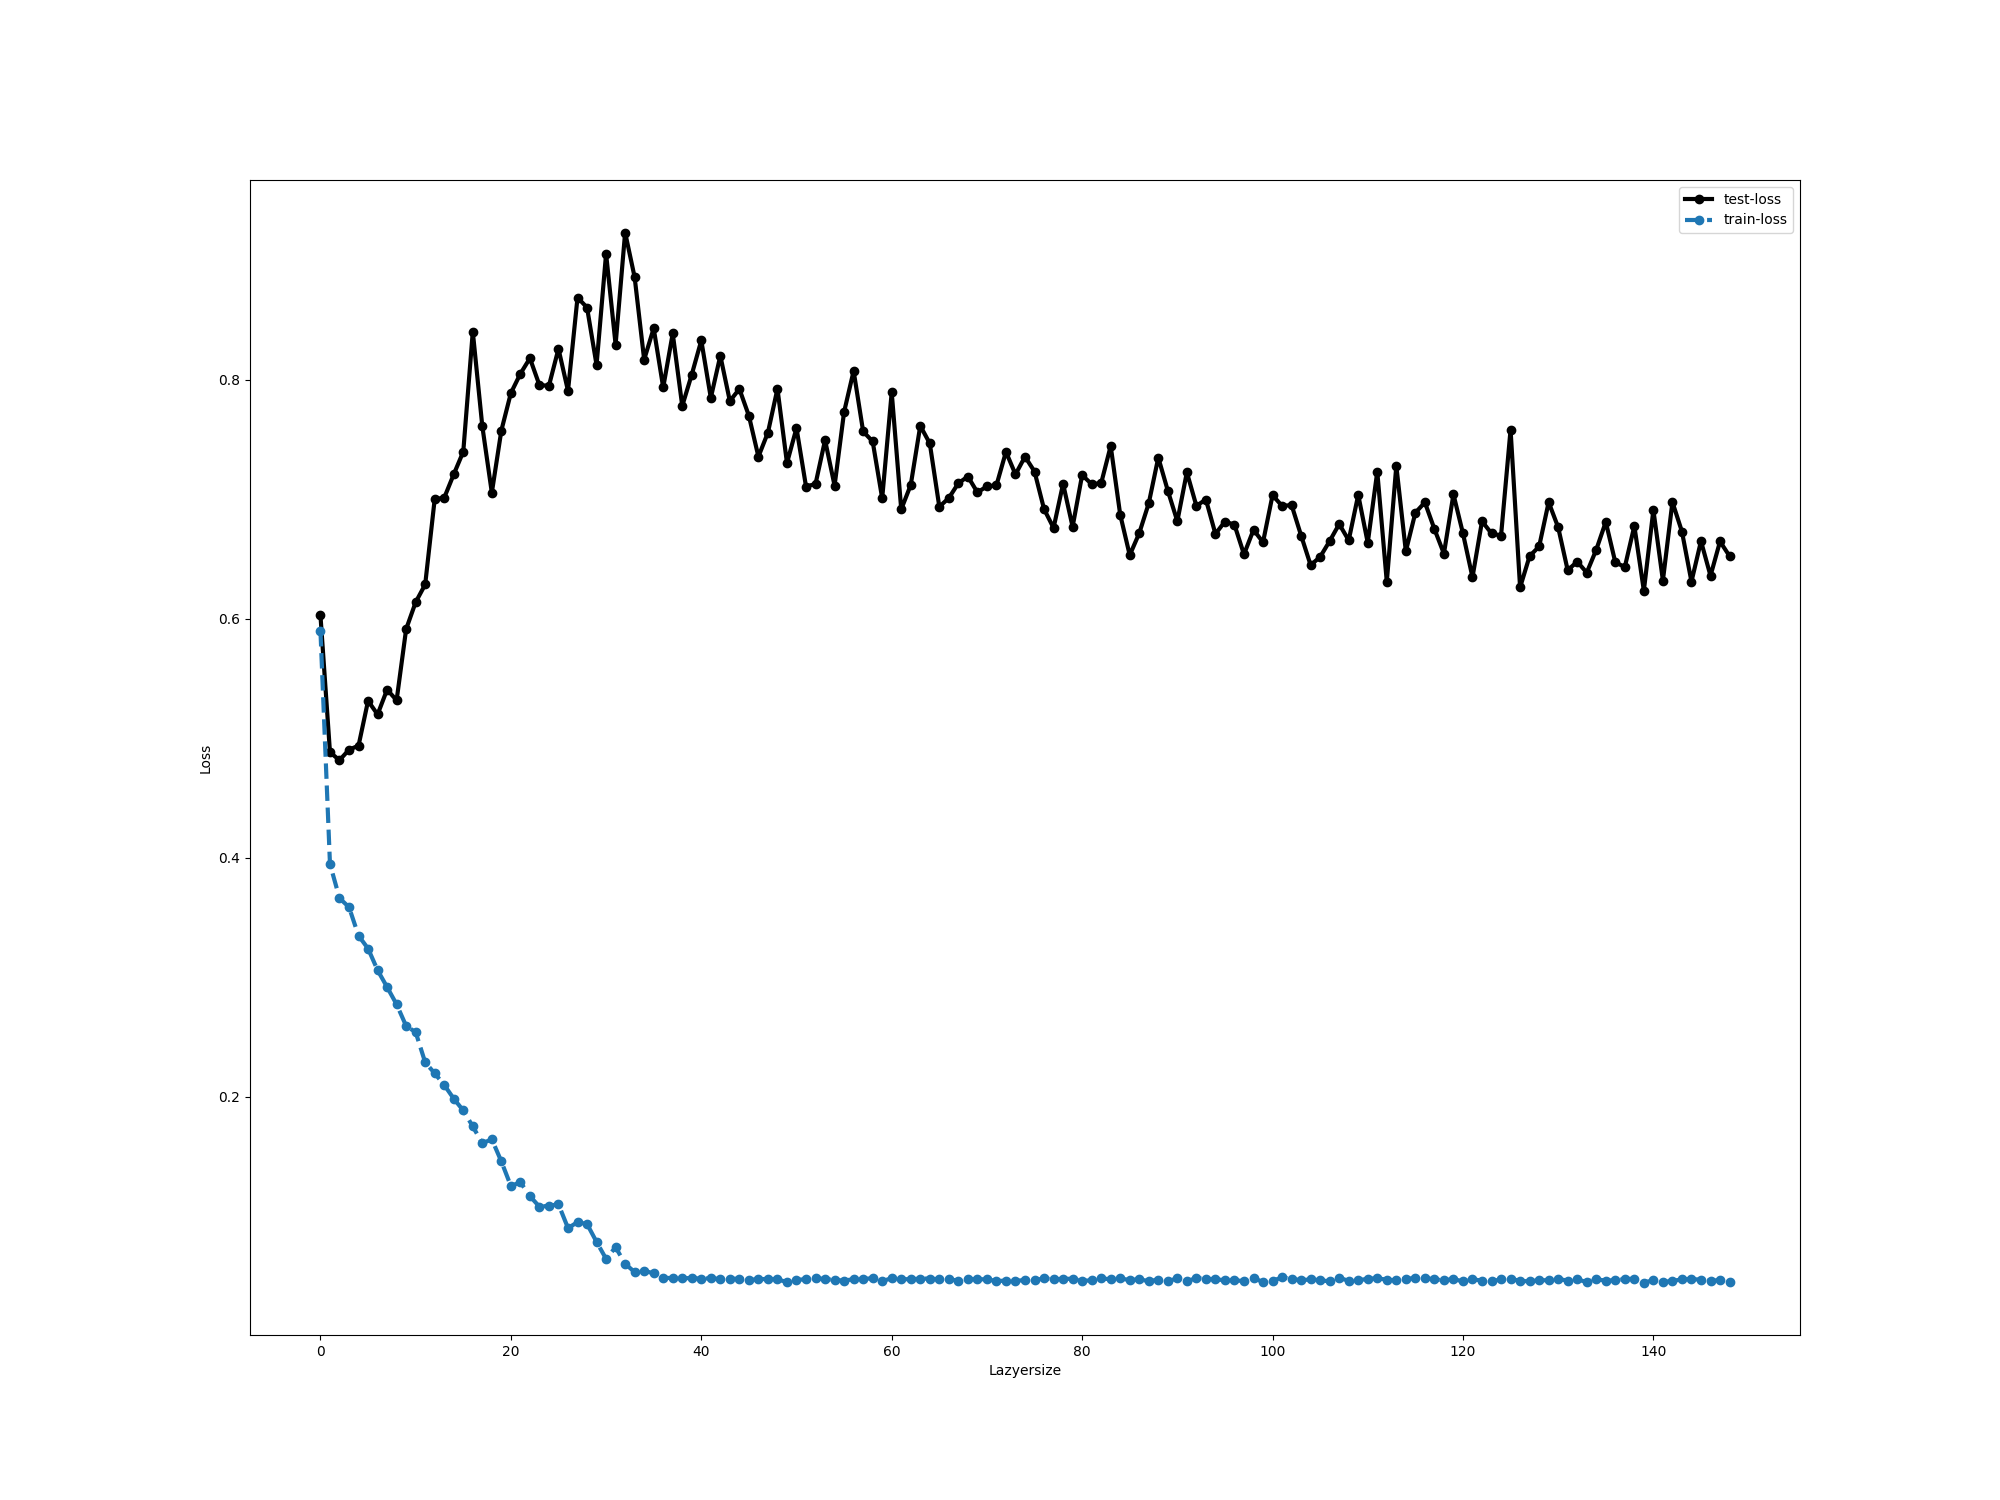
\includegraphics[width= 1\linewidth]{Abschlussarbeit_2021/LaTeX/images/double_descent_regression.png}
\caption{The loss was averaged over 5 runs. The loss at the interpolation threshold $(H \approx 35)$ is even larger than when one neuron is used in both layers. The performance after the interpolation threshold seems to be a lot worse as in the underparametrisized regime. Thus, it can be observed that the performance is not always better far in the overparameterized regime.}
\label{fig:double_descent_wine}
\end{figure}

\section{Observations Summary}

In following lines, we summarize what was observed in the previous experiments.
The following question will be addressed. To what extent is the behavior of the curve predictable if certain parameters are known?\\
The slope around the interpolation threshold, which is typical for the double descent risk curve, can therefore be traced back to different parameters. The peak of this slope is exactly where the training error reaches the value zero (\ref{double_descent_vanilla}).Therefore this peak receives the name "interpolation threshold". The peak takes higher values with stronger overfitting. Overfitting happens with a higher number of epochs, high learning rate or with more noise in the data set.  (\ref{fig:epochs_double_descent}, \ref{fig:Label_noise_on_double_descent}, \ref{fig:learning_rates_double_descent}). The larger $H$ is at the interpolation threshold, the wider is the slope around the interpolation threshold.  This is caused by larger sample size (\ref{fig:sample_size_double_descent}), increased noise (\ref{fig:Label_noise_on_double_descent}) or smaller number of epochs (\ref{fig:epochs_double_descent}). \\
With lower noise, there is a point where over-parameterized networks perform better than smaller under-parameterized ones. This is however not always the case. For example, for the wine quality data set, the test loss in the overparameterized region was significantly worse (\ref{fig:double_descent_wine}) than in the underparameterized region. So using the largest possible network and interpolating all the data is not necessarily the best solution. It is also important to note that the network architecture and the choice of parameters are not optimal for the best possible performance.\\
It was also found that the double descent phenomenon can occur with different network architectures, optimizers, data sets and loss functions. It is therefore worthwhile to investigate the phenomenon further.
Possible reasons why changing the attributes has the described effect will be taken up again in chapter \ref{Discussion}. After the phenomenon is further investigated with various experiments.



\chapter{Investigations and possible Explanations for the Behavior of the Curve}

In this section we will investigate the shape of the curve and take a closer look at some possible explanations for the double-decent-curve. Particular emphasis will be placed on how strongly overparameterized networks behave compared to weakly overparameterized networks. Thus, conclusions can be drawn regarding the better generalization of the large networks.

\begin{figure}[!htp]
\centering
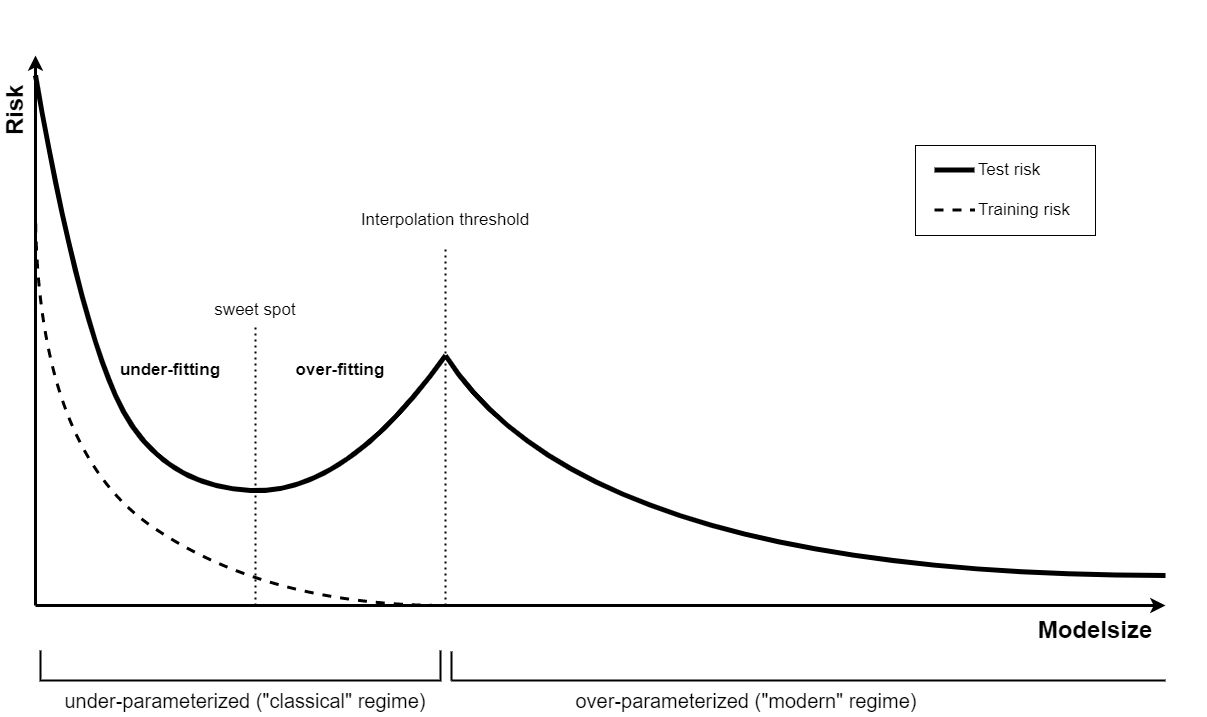
\includegraphics[scale=0.35]{Abschlussarbeit_2021/LaTeX/images/regimes_described.png}
\caption{shape of the double descent risk curve and it's designations based on the observation made in Chapter \ref{experimental_part}. The designations were made by \cite{belkin}. }
\label{double_descent_muster}
\end{figure}

To explain the phenomenon, we divide our risk curve into two regimes and try to find explanations for each regime. The first Regime is the under-parameterized regime, also called the classical-regime \cite{belkin} and the second regime is the over-parameterized regime, the modern-regime \cite{belkin}.\\
The behavior of the curve in the first regime is already well known and has also been well researched. The explanation of the shape is based on the bias-variance trade-off \cite{belkin}. We will mention this briefly in the next subsection, also because this is well known theory.\\
In the following subsection we will deal with the modern regime, i.e. the overparameterized regime. As we have already noted in the previous chapter, these two curves are separated by a peak, also called the interpolation-threshold. This is reached when the model is rich enough to perfectly memorize the training data i.e. the training error is zero. The behavior of the double-decent-risk-curve is easier to explain if we consider these two regimes separately and then put the findings together. As announced in the introduction, the second regime is not so well researched yet. Therefore, a clear and unambiguous explanation cannot yet be given. Nevertheless, in the section \ref{possible_explanations} possible reasons are mentioned, which might contribute to the behavior of the curve.  


%%%%%%%%%%%%%%%%%%%%%%%%%%%%%%%%%%%%
%%%%%%%%%%%%%%%%%%%%%%%%%%%%%%%%%%%%
%%%%%%%%%%%%%%%%%%%%%%%%%%%%%%%%%%%5
%%%%%%%%%%%%%%%%%%%%%%%%%%%%%%%%%%%%
\newpage
\section{Under-parameterized Regime}
\label{under_para}

In this chapter, the under-parameterized regime will be discussed. The analysis is more concise than that for the overparameterized regime. This is due to the fact that the behavior of the double descent curve is not as surprising as in the overparameterized regime and also follows well known statistical theories. A fundamental principle for the explanation of the behavior is provided by the bias variance decomposition \cite{belkin}, which will be explained in the following section.  

\subsection{The bias variance decomposition}
\label{bias_variance_chapter}

The bias-variance trade-off is responsible for the shape of the first curve. As already indicated in figure \ref{double_descent_muster}, there is a so-called sweet-spot, which balances bias and variance in such a way that the best possible performance of the model is achieved\footnote{If we only consider the classical regime}. Left of the sweet-spot, we talk about under fitting and to the right we talk about overfittig.\\
But first, we introduce the terms bias and variance. Let $(X^{*},Y^*) \subset X \times Y$ be a data set, $(X^{*},Y^*)  = \{(x_1,y_1),(x_2,y_2),\cdots (x_n,y_n)\}$. We want to find a mapping from $X$ to $Y$ via a Model. Let the real mapping be,
$$
y = f(x) + \epsilon \text{ with } y \in Y \text{ and } x \in X
$$
Where $\epsilon$ is an error, which arises because of noisiness for example in terms of measurement. The error is distributed around $0$ with a variance of $\sigma^2$. Assume our model, trained on $(X^{*},Y^*)$ finds a function $f^{*}(x): X \rightarrow Y$ so the expected error of our model is given by,
$$
Bias(f^*(x)) = E[f^{*}(x)] - f(x)
$$
This error is called the bias. $E[(f^{*}(x)]$ is the expected output given a random subset $(X^{*},Y^*) \subset X \times Y$.  So simply put, the bias is the expected difference between the predicted value and the real value. A high bias for example could occur, if we made a prediction whether a student will pass the exam only based on one feature in a given data set. The prediction based on only one feature could be quite inaccurate. The feature could be the amount of hours a student has studied.\\
The variance is given by,
$$
Var(f^*(x)) = E[(f^{*}(x) - E[f^{*}(x)])^{2}]
$$
 If the variance is high, the result of the model varies strongly depending on the selected training set or in many models also by the initial weights. This can happen quickly, for example, if a prediction takes into account features that are not meaningful. For example that the probability of passing the exam now somehow depends on the color of the hair. Because the given data set tricked the model into thinking that. Adding more and more features does make it easier to better predict the given training data. For unseen data points, however, this can be a hindrance, as patterns may have been seen in the training set that do not work for unseen data.

\begin{figure}[!htp]
\centering
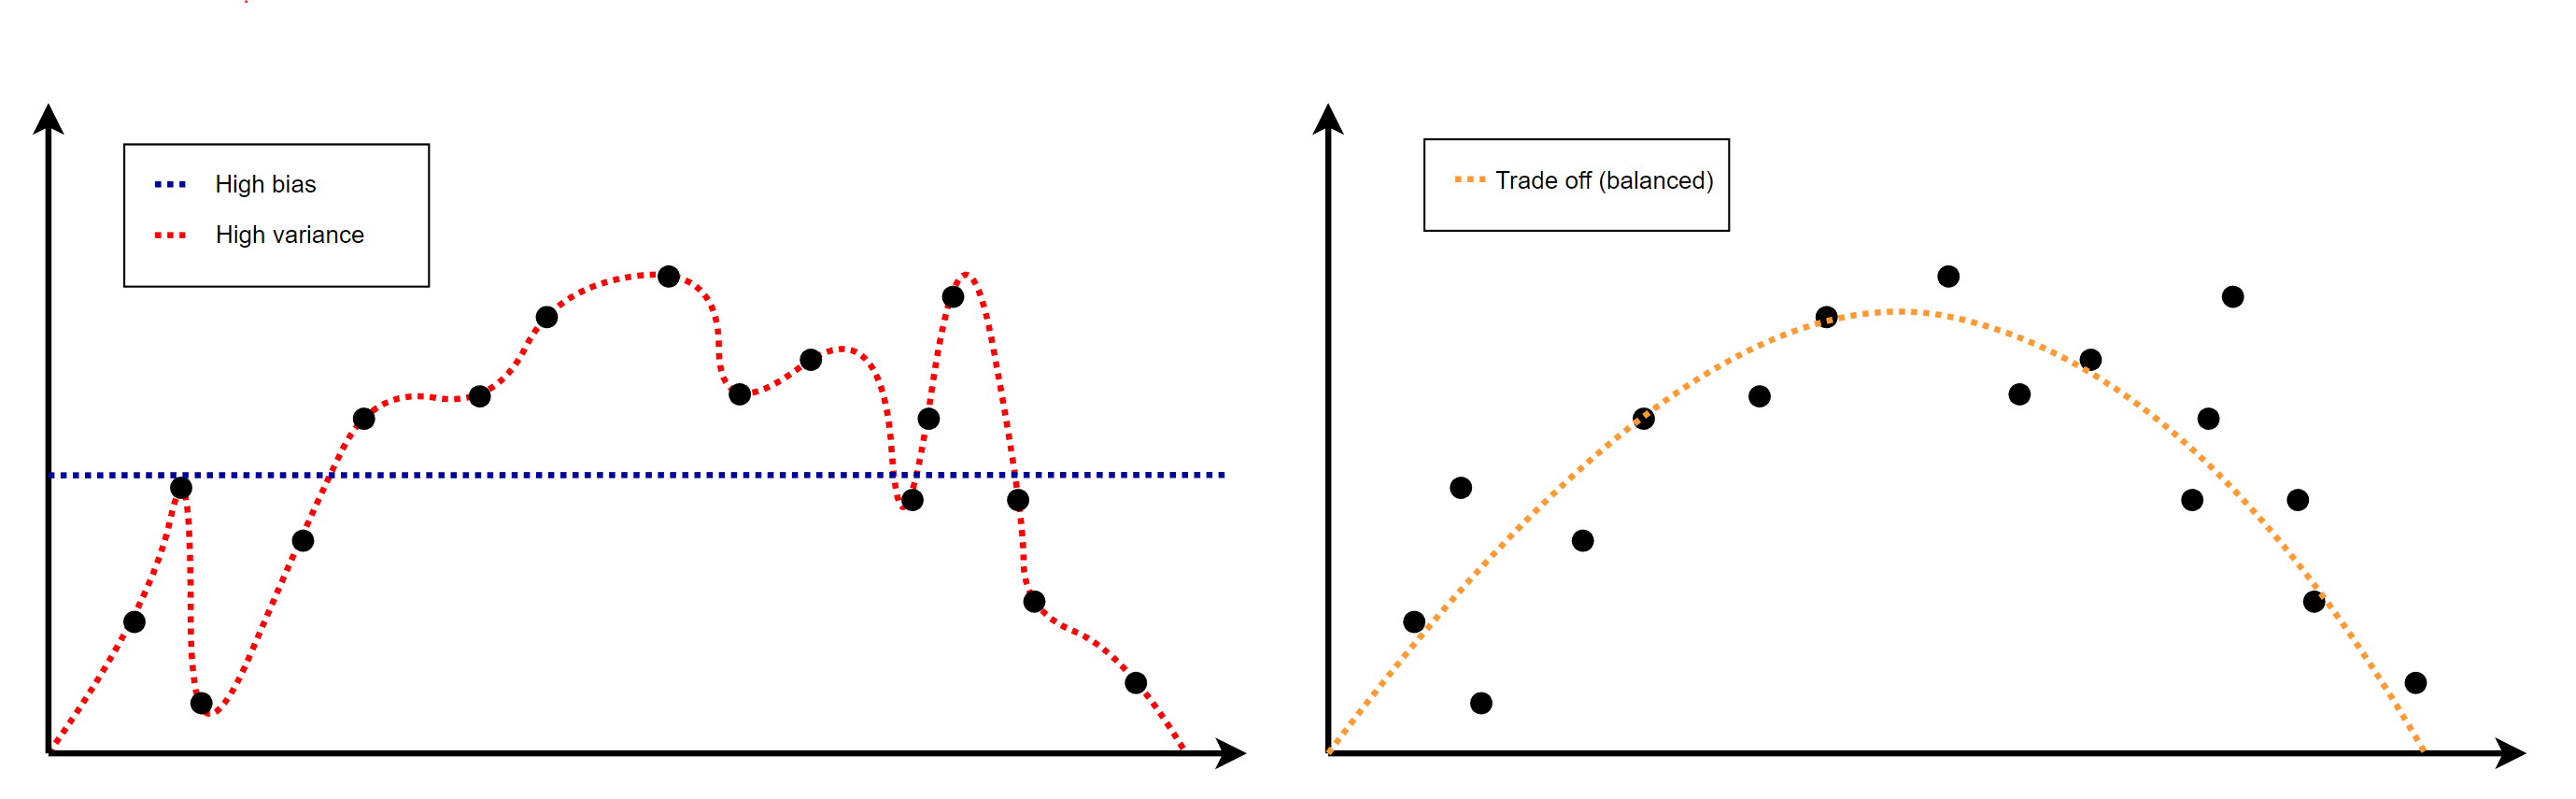
\includegraphics[scale=0.3]{Abschlussarbeit_2021/LaTeX/images/balances_function.PNG}
\caption{In the left graph we see two learned functions. The high bias function (blue) captures the training set inaccurately but is unlikely to change with in a new training process. For the high variance prediction, it is the other way around. On the right is a function that has a good trade off in terms of bias and variance. This prediction handles the noise very well and is also consistent with other training sets. }
\label{bias_variance}
\end{figure}

 We can generally say that if we have noise in the training set, which is usually the case, and the model tries to learn the training set perfectly, the noise is also learned and a high variance arises. This is classical overfitting.\\
Figure \ref{bias_variance} gives general idea of  the bias and variance trade-off. But how are bias and variance related? It can be assumed that if the lowest possible bias is desired, the variance becomes large and vice versa. For example, if a prediction of passing the exam is made based only on the number of hours studied, this prediction will not vary much with different training sets. The variance is therefore small. However, it will not be really accurate, because other attributes should be taken into account as well. Like for example the grades in other subjects. But if, on the other hand, we include many attributes into our decision, the prediction for an unseen data point will vary, as its decision depends on many features whose values themselves also vary. The variance becomes large, but the prediction of the model becomes more accurate averaged over all possible training-sets. However, a high variance can be bad for a prediction of unseen data. Therefore we have to find a trade-off. We try to represent this dependence mathematically. For this purpose the expected squared error\footnote{This is the loss function MSE (\ref{mse_eq})} of the model is considered, which normally should be minimized. 
$$
E[(y - f^*(x))^2] = E[y^2 + f^*(x)^2 - 2yf^*(x)] = E[y^2] + E[f^*(x)^2] - E[2yf^*(x)]
$$
We know that $E[X^2] = Var[X] + E[X]^2$ holds\footnote{This follows out of the definition of the Variance. For the proof see Appendix \ref{bv_help_eq}} so we can transform the Equation to, %%prove in appendix
$$
E[(y - f^*(x))^2] = Var[y] + E[y]^2 + Var(f^*(x)) + E[f^*(x)]^2 - E[2yf^*(x)]
$$
It holds that $E[y] = E[f(x) + \epsilon] = E[f(x)] + 0 = f(x)$. Because the noise is distributed around $0$. We can again rearrange the equation to,

\[ E[(y - f^*(x))^2] = Var[y] + Var(f^*(x)) + (f - E[f^*(x)])^2 \] 
\[\Longleftrightarrow E[(y - f^*(x))^2] = Var[y] + Var(f^*(x)) +  E[f -f^*(x)]^2 \]
Substituting the definition of bias and knowing that y has a noise that cannot be removed, we get,
\begin{equation}
    E[(y - f^*(x))^2] =\sigma^2 + Var(f^*(x)) + Bias(f^*(x))^2
    \label{bias_variance_eq}
\end{equation}


So now we have the relationship between the squared error, the variance and the bias, where $ \sigma$ is the variance of the value to be determined, an error which will always remain there. If we want to minimize the sqared-error $E[(y - f^*(x))^2]$, we have to find a balance between variance and bias. 
As already mentioned, the bias is low and the variance is high at high model complexity. Likewise, the bias is high and the variance is small at low model complexity \cite{wikipedia_bias_variance}. Adding the squared bias and the variance together, we get the curve of the first regime. The resulting Graph can be seen in figure \ref{fig:bv_decomposition}. This also explains many observations we have discovered in the previous chapter, in our experimental part.  \\
In the next section we will deal with the other regime. This starts directly after the interpolation threshold. Here, one should note with respect to the bias that it remains very small from here on \cite{pmlr-v119-d-ascoli20a}. With respect to the variance, one should ask what happens to it when we are in the over-parameterized region.


\begin{figure}[!htp]
\centering
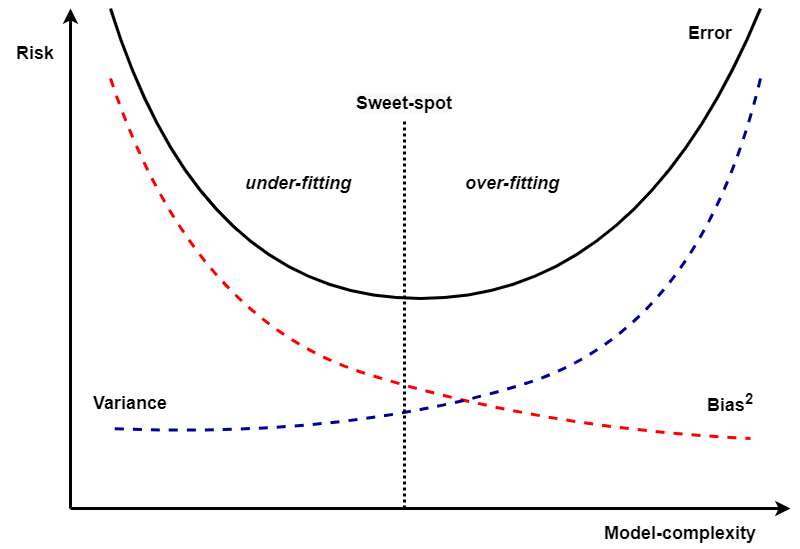
\includegraphics[scale=0.35]{Abschlussarbeit_2021/LaTeX/images/integral_bias_variance.drawio.png}
\caption{Resulting error curve. Finding the sweet-spot such that\\
$E[(y - f^*(x))^2]  = \sigma^2 + Var(f^*(x)) + Bias(f^*(x))^2$ is minimal.}
\label{fig:bv_decomposition}
\end{figure}

It is important to note that our presented decomposition of bias and variance was derived using the loss function "mean squared error" \ref{mse_eq}. However, the networks from chapter \ref{experimental_part} mostly use the loss function "sparce cross entropy" \ref{scc_eq}. A decomposition here is also possible here \cite{bias_variance_op}. This can be derived with the help of the Decomposition for Bregman Divergences. This can be seen in \cite{Bergman}.


%Hier noch einfügung, was man beobachtet hat und erklaren kann
%Abschlusssatz bezüglich varianz im anderen regime

%%%%%%%%%%%%%%%%%%%%%%%%%%%%%%%%%%%%%%%%%%%%%%
%%%%%%%                                   %%%%%
%%%%%%%%%%%%%%%%%%%%%%%%%%%%%%%%%%%%%%%%%%%%
%%%%%%%%%%%%%%%%%%%%%%%%%%%%%%%%%%%%%%%%%%%%
%%%%%%%%%%%%%%%%%%%%%%%%%%%%%%%%%%%%%%%%%%%%

\newpage

\section{Over-parameterized Regime} %rename maby
\label{over-p-regime}
Now there is only an explanation of the behavior after the first 'U' of the curve missing.
It was observed that models perform better and better from now on. From here on, the more parameters a model has, the better the model performs. In this chapter ideas or reasons shall be presented, why the curve decreases monotonously after the interpolation-threshold with increasing number of parameters. Particular emphasis will be placed on how strongly overparameterized networks behave compared to weakly overparameterized networks. Therefore the behavior of networks in the overparameterized regime depending on their size will be further investigated. Thus, conclusions can be drawn regarding the better generalization of large networks. At the end of the chapter, possible explanations for the second decrease of the curve are discussed.\\
An exact mathematical proof as in the underparameterized regime is not given here, as this behavior is still not sufficiently researched. However, a few heuristic explanations or ideas shall be presented.

\subsection{Experiments with random fourier features}
\label{RFF}
In order to get a feeling for the behavior of increasingly overparameterized networks, in the following section we will present three experiments in which different highly overparameterized networks are asked to solve simple problems. As shown in \ref{double_descent_vanilla}, the training loss for overparameterized networks is zero, which is why all training data is learned by heart.\\
For the experiments we resort to a famous class of non-linear parametric models, the Random Fourier Features (RFFs). RFFs can be viewed as a class of two-layer neural networks, where the first layer has random but fixed weights \cite{belkin}. The Model has to optimize the function 
$$
h(x) = \sum_{i = 1}^{N} a_{i}\phi(x,v_i)  \text{ where } \phi(x,v) := e^{i \langle x,v \rangle}
$$
the vectors $v_1,v_2, \cdots v_N$ are sampled independently from a normal distribution. \\
The first experiment is designed to solve a regression problem.
For the experiment, we create three different models, each with a different number of features. The first model has $N = 11$ features, the second model has $N = 30$ features and the 3rd model has $N = 50$ features.  \\
Our data set consists of 10 points $\{(x_0,y_0),(x_1,y_1),\codts ,(x_9,y_9)\} \in \mathbb{R}^2$.Where $y_{i}$ is the label of $x_i$. These 10 points represent a regression problem, which the models should solve. The 10 points are not chosen completely random. The $x$-values are fixed with $x_i = i+1$. The $y$-values $Y$ are normally distributed $Y \sim \mathcal{N}(\mu,\,\sigma^{2})$ with the parameters $\mu = a\cdot x_i +c$ and $\sigma = 1$. \\
We can see the deviation of $y_i$ as noise, because in the mean $y_i = a\cdot x + c$ holds. So we can easily say that the perfect function $f$ for predicting test data is $f(x) = a\cdot x + c$, since it would have the least deviation on infinitely many test data. So we can call $f^*(x) =a\cdot x + c$  the true function\footnote{for the prove see Appendix \ref{proof_for_1d_rff}}. \\
In our experiment all three models are rich enough to predict the data points exactly. This means that the learned function from the models will intersect all training points. We have a training accuracy of 100\% in all cases. We are therefore behind the interpolation threshold. The question now is which of the three models is closest to the true linear function $f^*$.\\
After performing the experiment, we can observe that the function learned from the model with many features is significantly smoother and has fewer deviations from the perfect function $f^*$. A more elegant and simpler regression function was found, which under the constraint to hit all training points. Of course, even if all the test points are passed, we can still say that the function with $N = 50$ features is not a bad function in terms of predicting test data.
The learned function from the model with only $N = 11$ random fourier features, on the other hand, is very poor and has large distance to the true function $f^*$. The regression problem is therefore solved very badly here. \\
 It can therefore be observe again that in the modern regime more is better. Repeating the experiment several times, the finding remains the same. The different learned functions can be observed in figure \ref{fig:1d_rff}. \\

\begin{figure}[!htp]
\centering
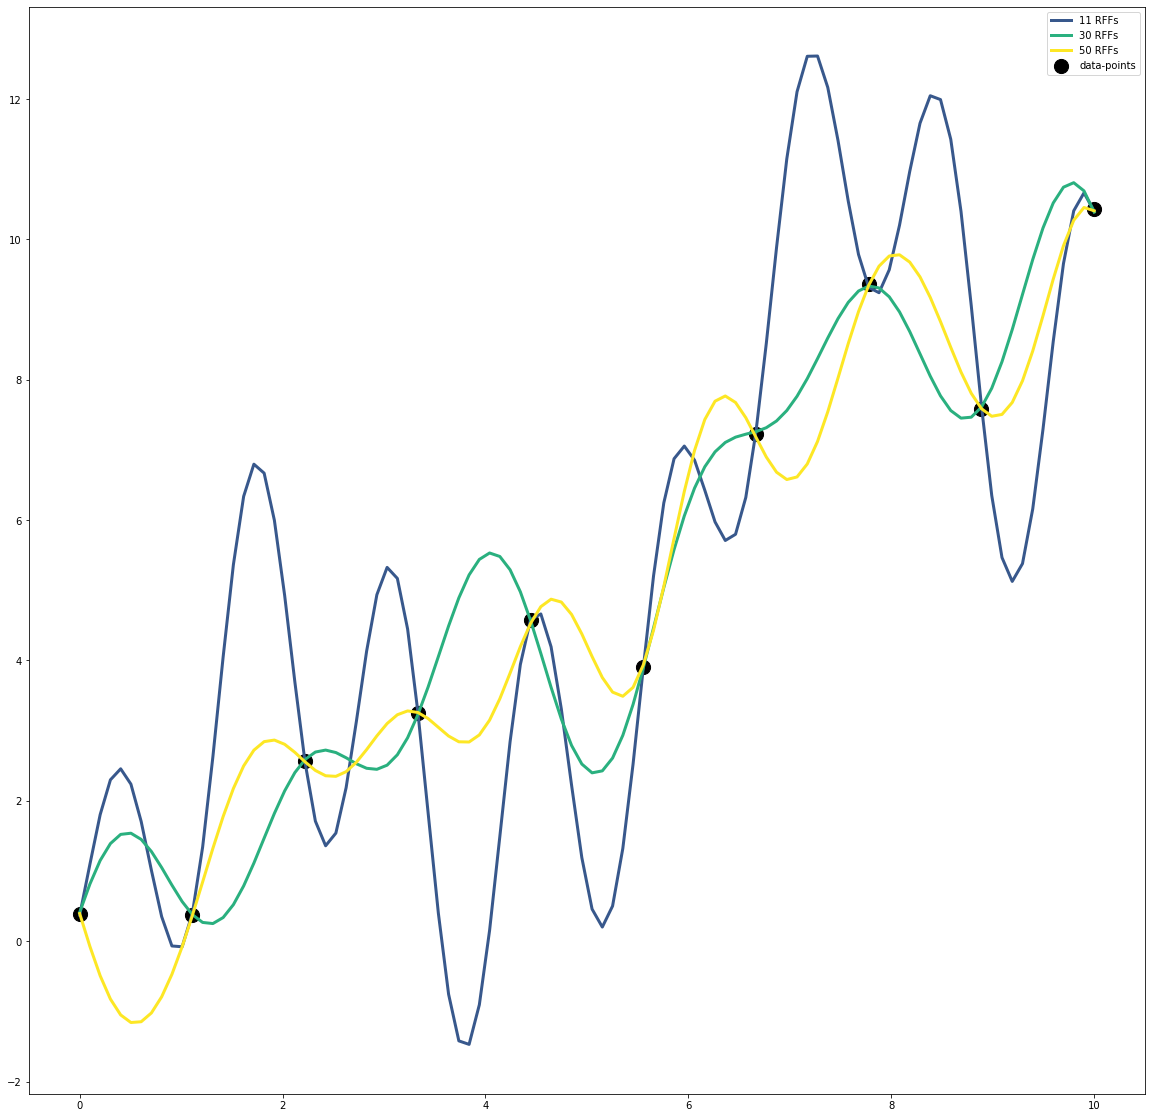
\includegraphics[scale=0.3]{Abschlussarbeit_2021/LaTeX/images/RFF_1d.png}
\caption{Three different solutions of a regression problem. The first function was predicted by a model with $N = 11$ RFFs, the second function by a model with $N = 30$ features and the third function by a model with $N = 50$ features. The linear function where the labels are sampled around is $f^*(x) = x$ }
\label{fig:1d_rff}
\end{figure}

\newpage

Two more examples which have a similar effect shall be presented.
The example from above has only shown a learned function from 
$\mathbb{R} \rightarrow \mathbb{R}$. But how does it look now, if a function maps from $\mathbb{R}^2 \rightarrow \mathbb{R}$? So we need three dimensions to represent the function. Can we observe a similar effect here?\\
To find out, a scenario similar to the one above was created. Again, a function is to be learned. this time it is the x-y plane so $f(x,y) = 0$.
The training-set consisted of 100 points, where the set of points is given by $A\times B$, where $A$ and $B$ are sets of 10 points, which lie between $-10$ and $10$ and all have the same distance to each other. Again the label has a little bit of noise to it. Each data point is normally distributed around the value $\mu = 0$ with a variance of $\sigma = 1$.\\
For this experiment, two RFF models were trained. One of them with $N = 120$ features, the other one with $N =10000$. Both again rich enough to interpolate all data points exactly.

\begin{figure}[!htp]
\centering
\begin{subfigure}{}
  \centering
  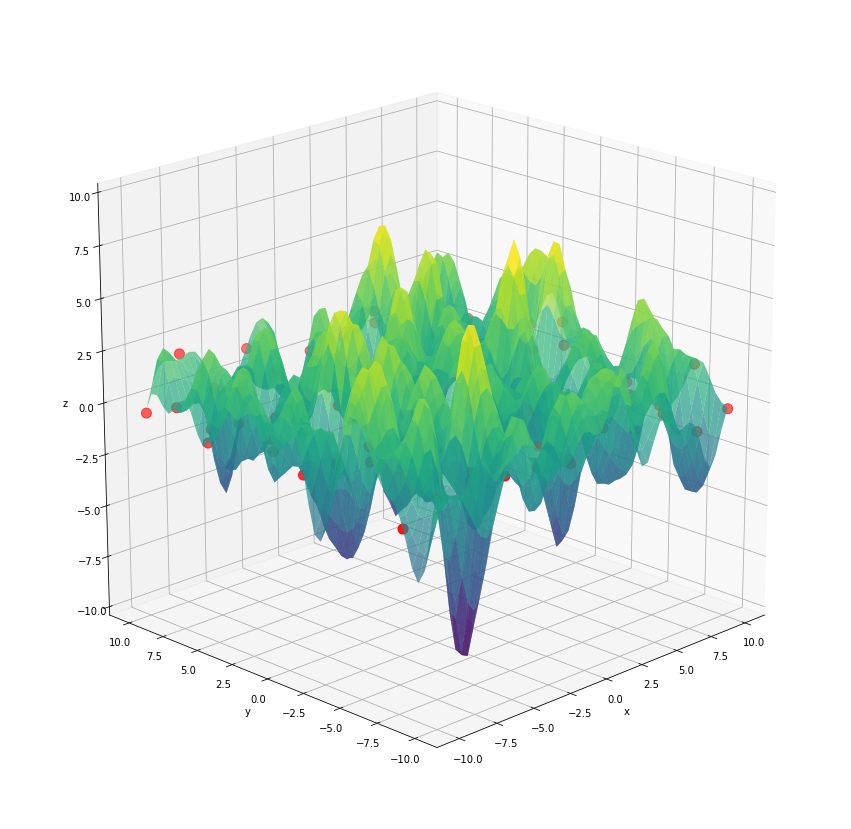
\includegraphics[width=.49\linewidth]{Abschlussarbeit_2021/LaTeX/images/120_RFF_3d.png}
  \label{fig:sub1}
\end{subfigure}%
\begin{subfigure}{}
  \centering
  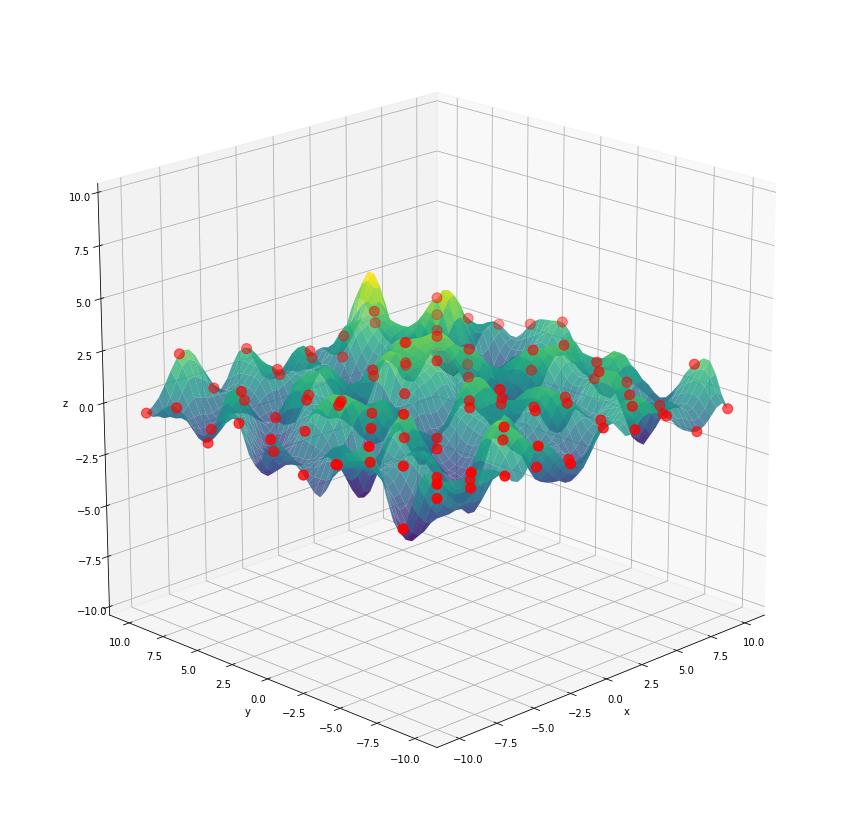
\includegraphics[width=.49\linewidth]{Abschlussarbeit_2021/LaTeX/images/10000_RFF_3d.png}
  \label{fig:sub2}
\label{fig:high_varianz_with_noise}  
\end{subfigure}
\caption{The left plot shows a function learned from a model with $N = 120$ random fourier features. The right plot shows the function learned by a model with $N = 10000$ features. The red points are the data-points.}
\label{3d_RFF}
\end{figure}


We also make the same observation in the multidimensional. The model with the larger number of parameters performs better again. For the same reason as in one dimensional case. The learned function is softer and has not so high peaks, which deviate from the plane $f(x,y) = 0$. Again, repeating the experiment does not provide different results. It is also interesting to note that if a larger grid is to be predicted with $A\times B = [-20,20]\times [-20,20]$, the extrapolation of these points is also significantly better for large models. This can be observed in the Appendix \ref{extrapolation}.

So far we have seen the effect in regression models. But how does it look now in the case of classification? \\
For this reason, a simple decision problem was constructed. On a grid with $20 \times 20$ points, the data is divided into two classes, $red$ and $blue$. The Probability, that a point $(x,y)$ where $(x,y) \in [-50,50] \times [-50,50]$ gets assigned to the red class, is given by
$$
P(red| x,y) = 1 - P(blue| x,y) = \begin{cases}
1 - \frac{1}{(2+ \frac{2}{5}|x|)} & \text{if } x < 0\\
\frac{1}{(2+ \frac{2}{5}|x|)} & \text{if } x \geq 0 \\
\end{cases}\\
$$
All points have the same distance to each other. The data-points $(x,y)$ where $x \geq 0$ and $x$ gets assigned to $blue$. Can be interpreted as noise. We note that a simple separation in the form of a line would be very efficient here. The vector $w = (0,1)$ would be a very good choice, and would perform well, even best possible, on this classification problem. \\
Again, we train two models. Both are rich enough to learn all training data perfectly. So we are again to the right of the threshold. Our supposedly weak model has $N = 300$ RFFs, whereas the strong model has $N = 20000$ features.
We see very clearly in this experiment that, again, the richer model solves the task better. In this case even clearly better, because we see that the model with $N = 300$ features will perform very poorly on new test data. 
The model with $N = 20000$ features, on the other hand, can be expected to have a solid performance with new data. We also make two other interesting observations. First, the decision surface of the model with fewer features is much finer and consists of many small spots, whereas the decision surface of the model with $N = 20000$ features consists of large areas. The rich model therefore is much more confident about its decisions. Here there are hardly any white areas. With the help of the much more complex model a much simpler function was found. \\

\newpage

\begin{figure}[!htp]
\centering
\begin{subfigure}{}
  \centering
  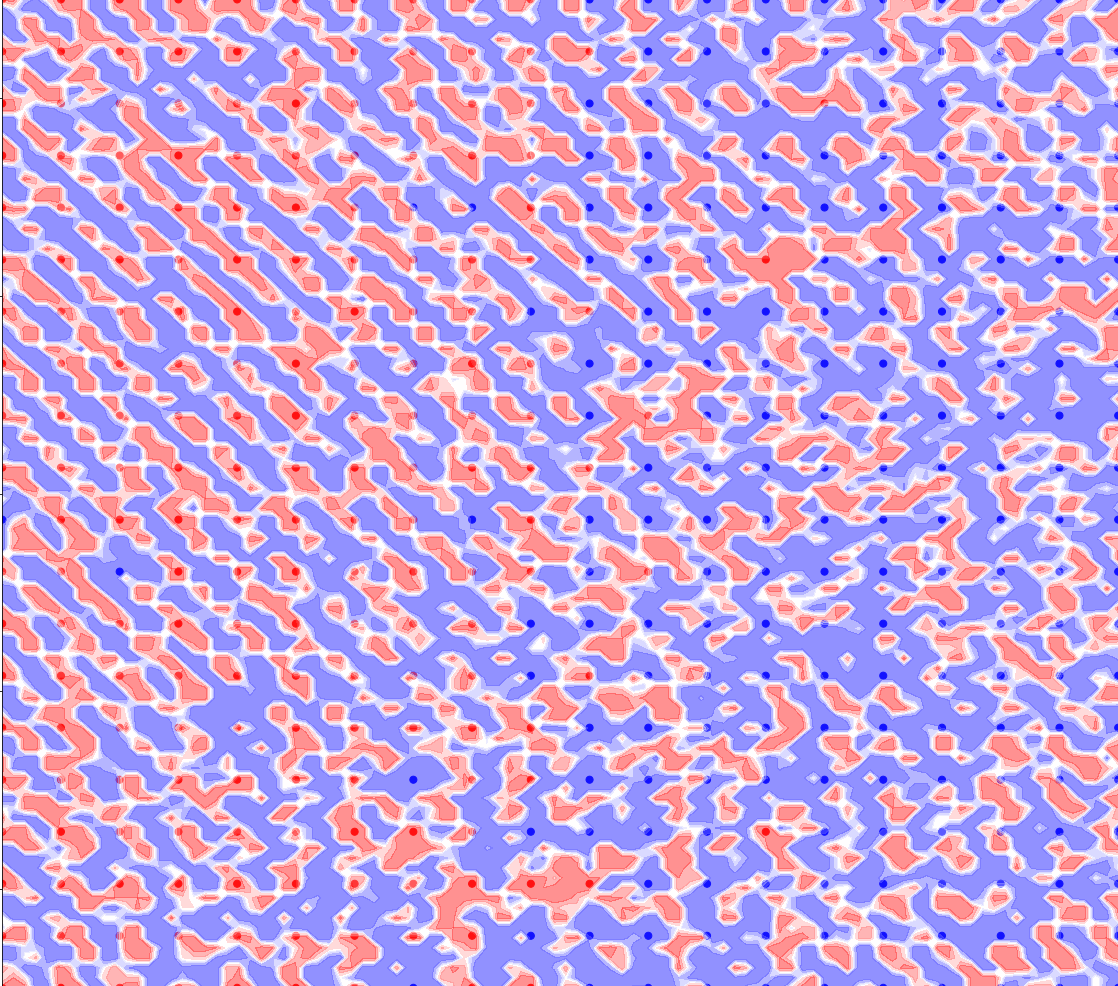
\includegraphics[width=.42\linewidth]{Abschlussarbeit_2021/LaTeX/images/Decision_Surface_less_features.png}
  \label{fig:sub1}
\end{subfigure}%
\begin{subfigure}{}
  \centering
  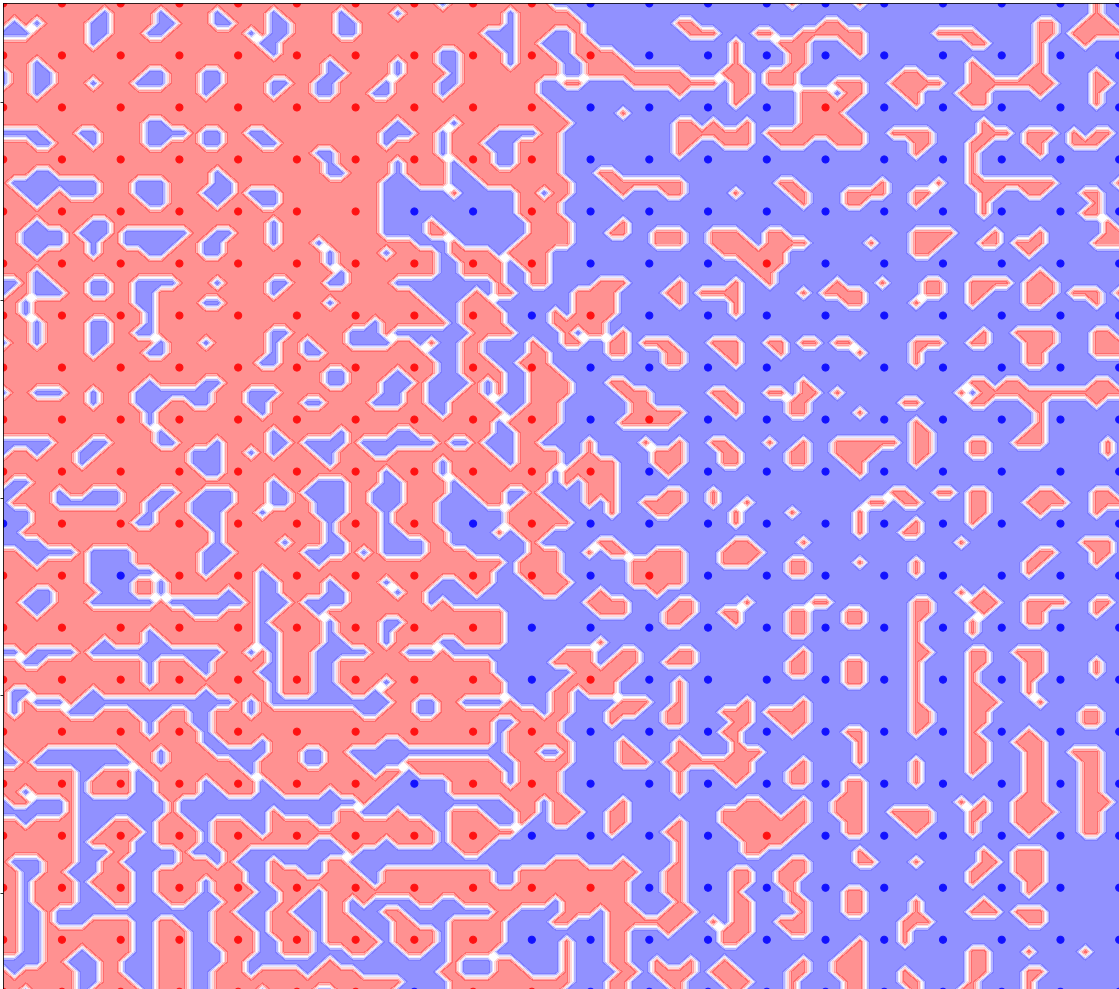
\includegraphics[width=.42\linewidth]{Abschlussarbeit_2021/LaTeX/images/Decision_Surface_many_features.png}
  \label{fig:sub2}
\end{subfigure}
\caption{On the left is a decision surface from a model that has $N = 300$ RFFs. The right image shows a decision surface created by a model with $N = 20000$ features. A new point on the grid would be classified according to the color of the decision surface. The intensity of the color indicates how sure the model is. For a point $(x,y)$ in a white surface $P(blue|x,y) = P(red|x,y) = 0.5$ would apply.}
\label{decision_RFF}
\end{figure}

We can now summarize what was observed. The more features the Models have, or the more neurons the Models have, the smother the learned function of the model. So it is easier for the network to find a suitable approximation of the real function of the problem. The more complex our model is, the simpler and more elegant the solutions we find. One could also say that the network focuses not only on learning the training data perfectly, but also on recognizing patterns in the data set itself. With increasing number of parameters the model gets a kind of feeling for the shape of the data. In the literature this effect is called inductive bias \cite{wikipedia_inductiv_bias}.
It also stands to reason that the variance between learned functions described in \ref{bias_variance} is smaller for larger networks. This is because as the number of parameters increases, the functions get closer and closer to the "true function" $f^*(x)$. 

\newpage

\subsection{Other interesting discoveries}

Apart from the function resulting after the training, other interesting observations can be made. In this subsection, the weights of the networks will be examined in more detail. How do the individual weights change when a significantly larger number of parameters is present?\\
Subsequently, the bias and the variance will be discussed again. How do these two factors behave in the overparameterized range? After all, the equation \ref{bias_variance_eq} established in the last section must still hold regardless of the model size.\\
%%maby delet it and mention it in the explanation
In this subsection an experiment on found minima depending on the initialization of the weights should also be done. Here observations can be made, what initialization of weights can have for an influence on the learned function.\\
At the end, the shape of the loss function is to be examined. Here we will not go too much into details. But there is no doubt that found minima depend strongly on the behavior of the loss function. What happens if the loss landscape, i.e. the graph of the loss function, is smoothed? 



\subsubsection{Training steps and weight change in the overparameterized regime}

When training the models in Chapter \ref{experimental_part}, it was noticed that a minimum is found much faster with large models.  This is because the model does not need so many adjustments to the weights until a suitable minimum is found. A plausible assumption would be that weights do not take on values that are too extreme, since a minimum can be found for rich models even without changing the weights too much. \\
So, can we possibly establish a connection in the overparameterized regime between the generalization of the model and the number of epochs needed to reach zero training error? For this purpose, we perform another experiment. In this experiment we want to investigate how many epochs are needed to reach $0.01$ training loss depending on the network size. We also consider the average change of a weight in the network graph. So the average difference between the initialization and the value of the weight after training. \\
For the experiment, we use a fully connected neural network\footnote{similar to \ref{model equation}} with a hidden layer consisting of $1 \leq H \leq 80$ neurons. We are  training on a Subset of MNIST with $15000$ Samples. Stochastic gradient descent is used with a learning rate of $\eta = 0.1$.
The Training stops if a training loss below $0.01$ is reached or 200 epochs where processed. To reduce the number of factors observed, the biases are fixed to the value $0$ and thus cannot be learned.The initial weights $W$, on the other hand, are normally distributed with
$$
W \sim \mathcal{N}(0,\,0.05)
$$
It can be observed that a high correlation exists between the test lost, the number of epochs required and the average weight change. This can be seen in figure \ref{avg_weightchange}. Since the experiment here was performed only once and thus fluctuations in the test loss were not straightened out, it can be observed that even fluctuations in the number of epochs required have an influence on the test loss. It is quite clear here that after the interpolation threshold ($H = 11$) test loss, the number of epochs and the average weight change decrease monotonically.  \\
The fact that for larger models the average weight change is small, is very interesting. It shows that the model can find a minimum by a few simple weight adjustments, if it has enough capacity. \\
In figure \ref{density_weights} density functions for the initial weights, the weights after the training process and the density function of the weight change are shown.
A total of four different complex models with $H \in \{11,20,100,1000\}$ have been investigated. All four models are in the overparameterized region, as figure \ref{avg_weightchange} shows. On the left side of the figure it can be observed that the variance of the learned weights becomes smaller and smaller for larger models.
The density function for the weights after training becomes smoother and smoother for large $H$. This observation can be explained by the behavior of the Gradient Descent algorithm. With a high number of parameters, the loss function depends on significantly more parameters. An activation of a neuron can thus be forced by many small changes, since the dendritic potential is composed of significantly more weights. \\
On the right side of \ref{density_weights} it can be observed that the amount of weights, which were strongly adjusted during the learning process, strongly decrease with the size of the model. In addition, the density function becomes more and more compressed towards zero as $H$ becomes larger. \\
Thus, large networks have the advantage that SGD finds a minimum here, which can be realized only by small adjustments of the weights. This might prevent large variances in the learned weights. A possible conclusion would be that minima varying significantly in performance are found depending on the initialization, as individual weights are changed more. We explore this assumption a bit more in the next section \ref{possible_explanations}. It should also be noted that with a higher number of parameters, more minima with zero training loss can be found. This also influences the convergence of SGD.  
\\



%%TODO: Bild von bsp verteilung in Anhang


%%%%%%%
%%wirte about weightclustering here and mention the unsufficiant exploration RESTRUCTURE!!!!
%%%%%%%



\begin{figure}[!htp]
\centering
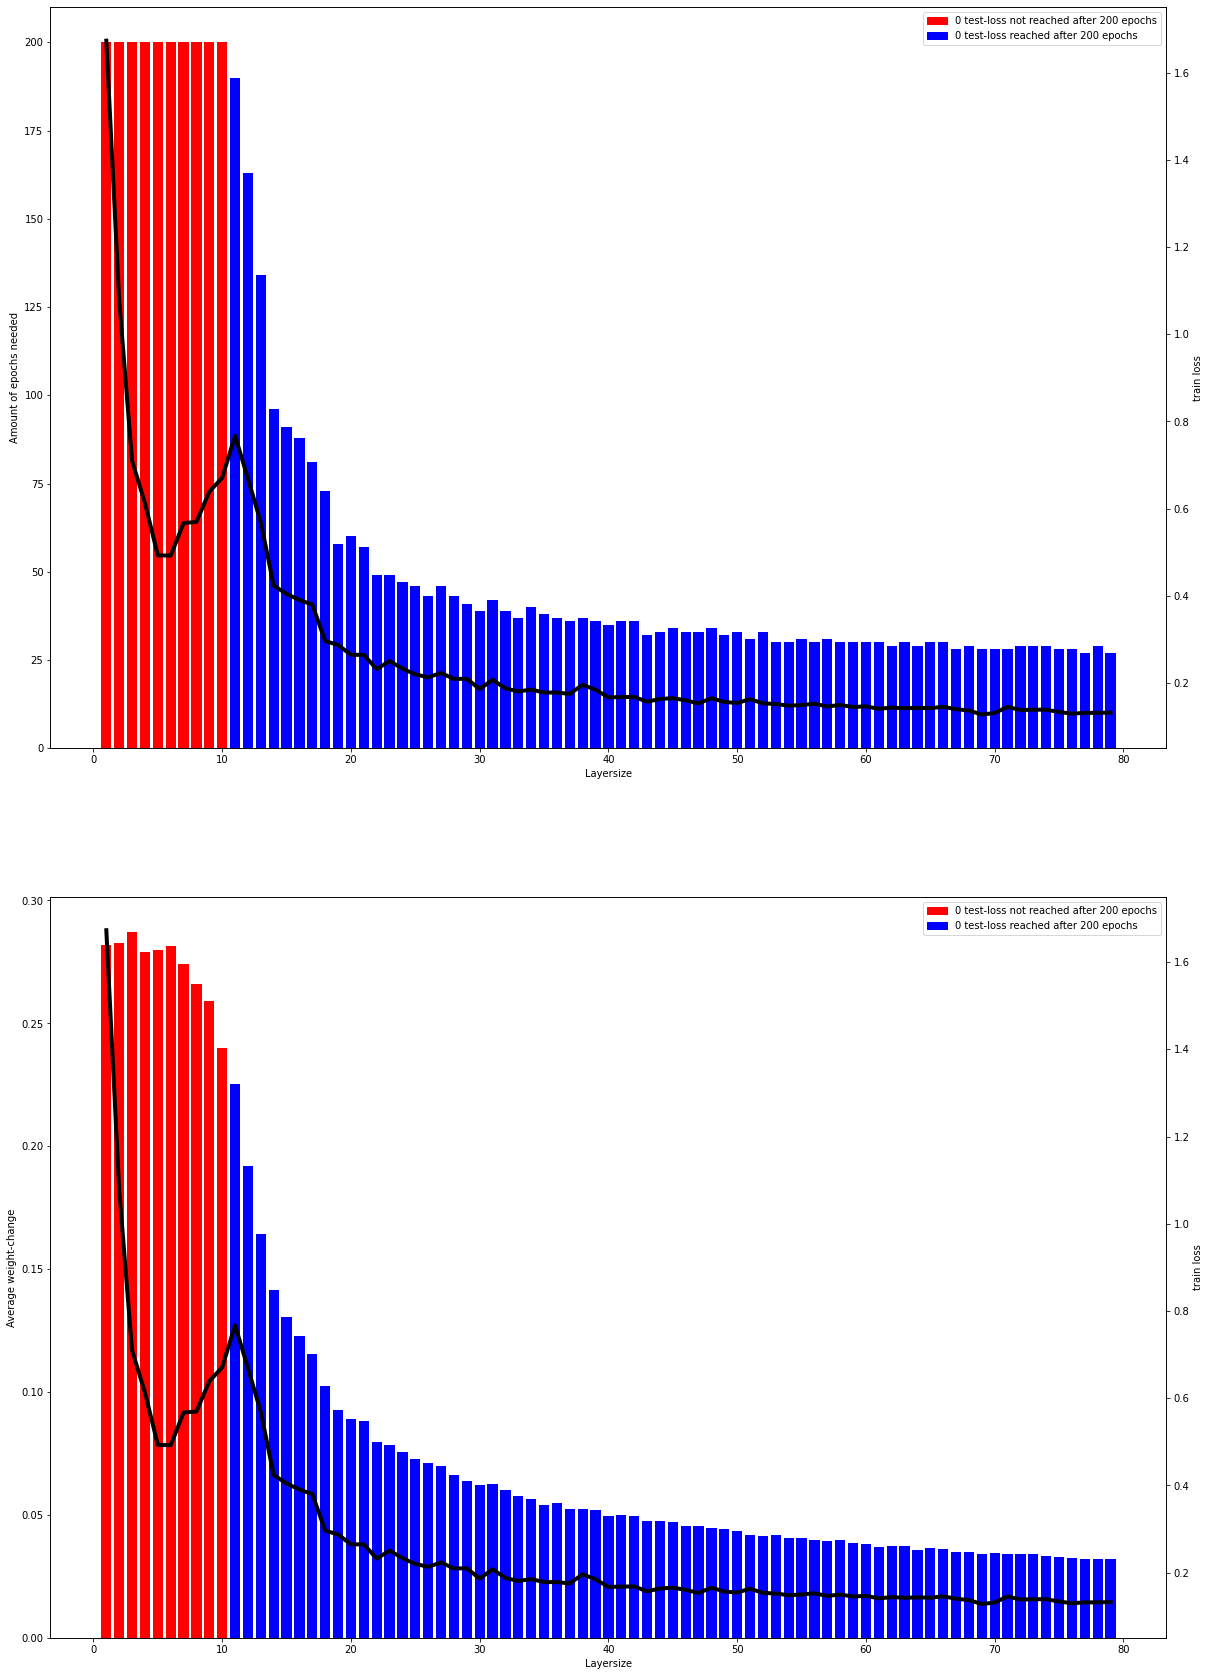
\includegraphics[scale=0.3]{Abschlussarbeit_2021/LaTeX/images/epochs_needed_15k.png}
\caption{The upper half shows the number of epochs needed for a train loss of $0.01$ (blue bars). The black function describes the test loss. Double descent is clearly visible. \\
In the lower half you can see the average change of a weight.  Here the bar is blue again, after the interpolation threshold has been passed.}
\label{avg_weightchange}
\end{figure}
%todo: find a good description (something about correlation)
%%model is simpler, SGD finds minima more easily


\begin{figure}[!htp]
\centering
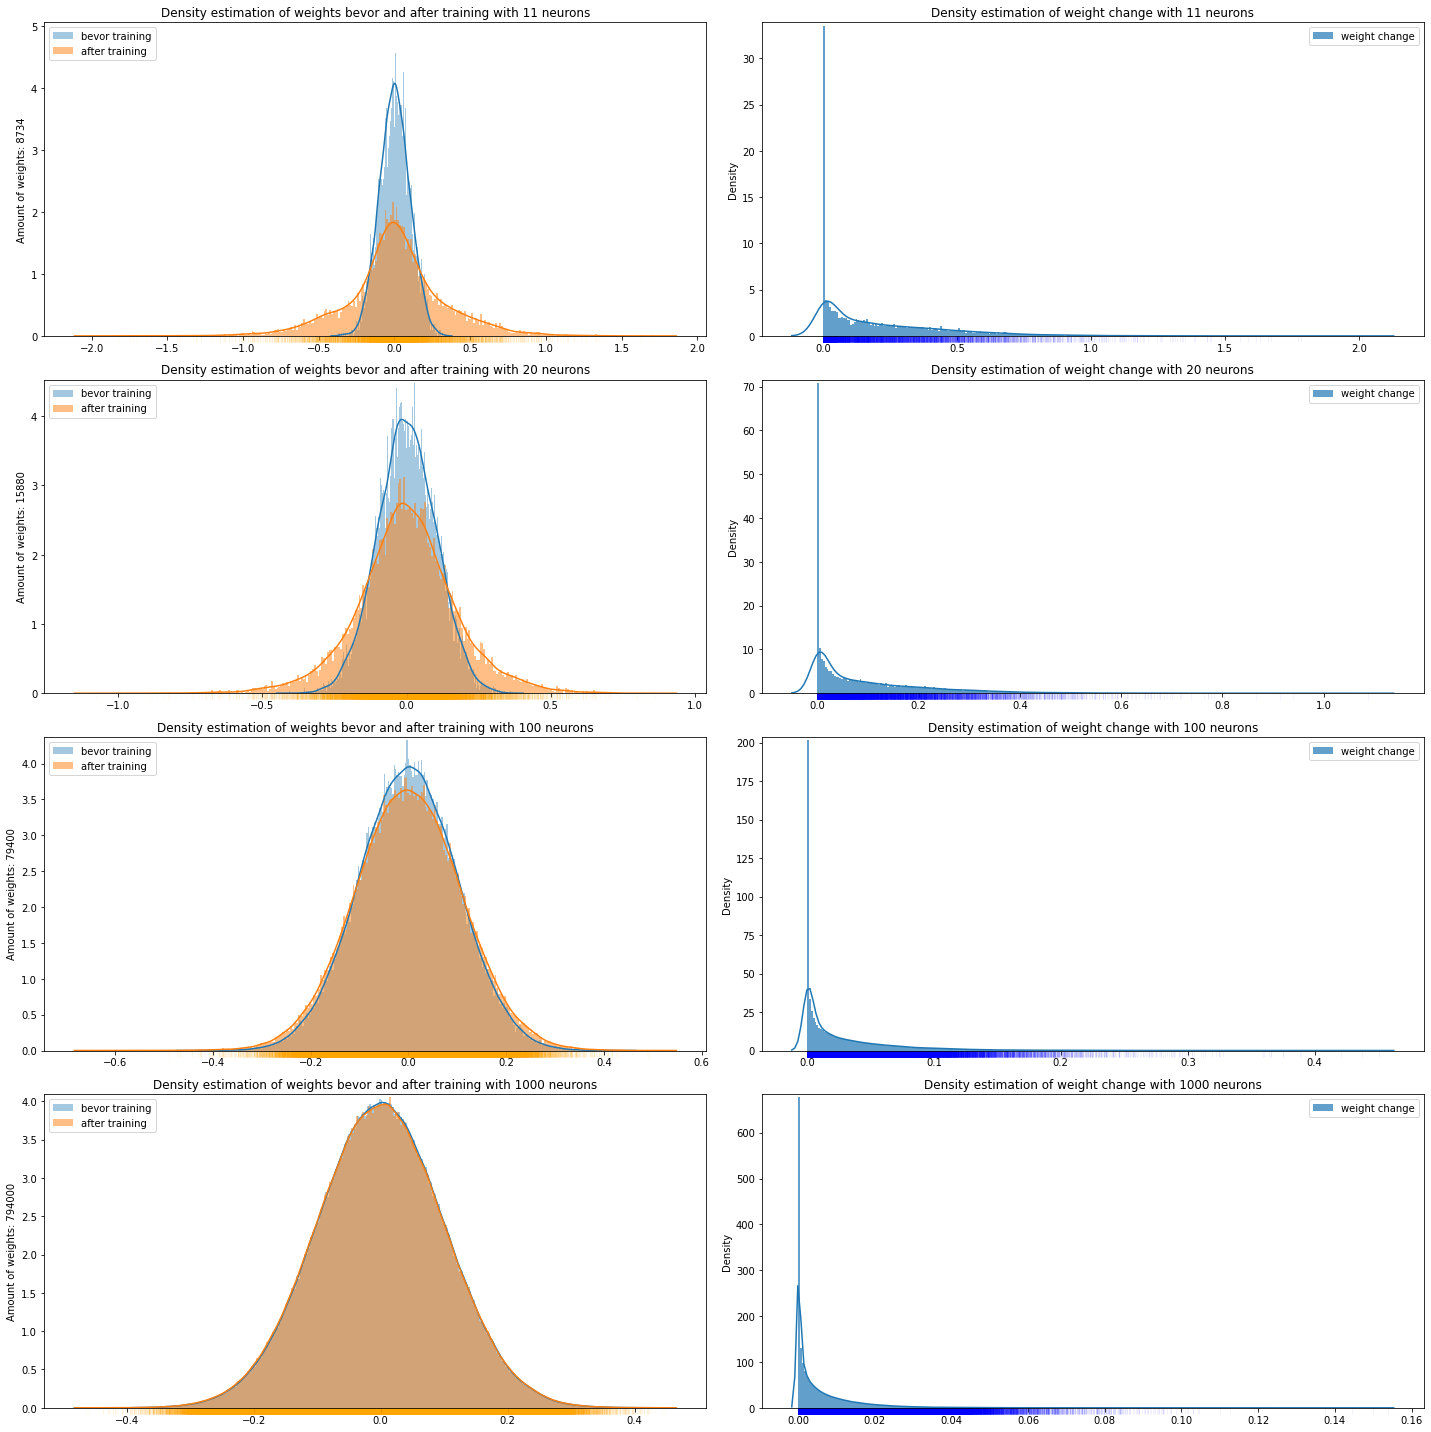
\includegraphics[scale=0.3]{Abschlussarbeit_2021/LaTeX/images/Weightdist_15k_sns.png.png}
\caption{On the left side you can see the density function of the weight values in the network. Blue shows the weights before training and orange shows the weights after training. \\
On the right side is shown the density function of the weight change.  }
\label{density_weights}
\end{figure}

\newpage


\subsubsection{Bias and variance in the overparameterized regime}

In chapter \ref{bias_variance}, we discussed bias and variance in the underparameterized regime. But what happens to bias and variance in the overparameterized regime? Regardless of the size of the network, equation \ref{bias_variance_eq} must still hold \cite{bias_variance_op}. 
The squared error is still dependent on bias and variance. Since we always interpolate the data perfectly in the overparameterized domain, for a learned function $f^*(x)$ trained with data from the real function $f(x)$ , it holds that 
$$
Bias(f^*(x)) = E[f^*(x)] - f(x) < \epsilon  \text{  }  \forall x \in X, \epsilon > 0
$$
So a consistently low bias and a decreasing test loss with the increase of $H$ must ensure that the variance of $f^*(x)$ must decrease. \\
Figure \ref{varianz_mnsit} gives evidence for this experimentally. Here the distribution of the test-loss and the test accuracy of two different models $M_{H = 12}$ and $M_{H = 300}$ with the architecture of equation \ref{model equation}, trained to zero training error can be seen. Both are in the overparameterized regime. However, $M_{H = 12}$ is just past the interpolation threshold. The learned functions of $M_{H=12}$ vary significantly more in their performance on the test data set. In contrast, the variance of the performance of $M_{H=300}$ is very small. The varying performance is strongly related to the varying of learned functions. It can be assumed that the following inequality applies.
$$
Var[f^{(300)}(x)] < Var[f^{(12)}(x)]
$$
Where $f^{(k)}$ is the learned function of a model with $H = k$ neurons in the hidden layer. \\
Similar observation is made in \cite{pmlr-v119-d-ascoli20a} and \cite{bias_variance_op}. In \cite{pmlr-v119-d-ascoli20a} the variance is further subdivided into initialisation variance, noise variance and sample variance. It was shown with a Random Feature model\footnote{more information about the used architecture can be found in \cite{RF-model}} there that at the interpolation threshold, the inizialization variance and the noise variance peaks extremely at weak regulating \cite{pmlr-v119-d-ascoli20a}. If the weights are regulated more, the now somewhat weaker peak at the interpolation threshold is solely due to the initialization variance and the noise variance \cite{pmlr-v119-d-ascoli20a}. The decomposition can be also viewed in figure \ref{fig:varianz_ascoli}. \\
The initialization of the weights can therefore play a large role. This can be also observed in more detailed example\footnote{The source is an article which shows that large variances in performance occur with few weights available. It also describes what influence the addition of more weights has \cite{double_descent_2021_splines}} in \cite{double_descent_2021_splines}. 
Also the sampling variance peaks here. Depending on the training data, the learned function can vary very much. 
Crucially, however, both of these variances decrease sharply after the interpolation threshold \cite{pmlr-v119-d-ascoli20a}. Thus, the model is more robust against varying initialization and against varying order of training data. The resulting total variance decreases as described above. In \ref{varianz_mnsit}, the same order of training data was always used, which makes the described sampling variance disappear. 
This finding also fits well with the observations from section \ref{RFF}. A simpler smoother function cannot vary as much as a complicated function with strong peaks.

\begin{figure}[!htp]
\centering
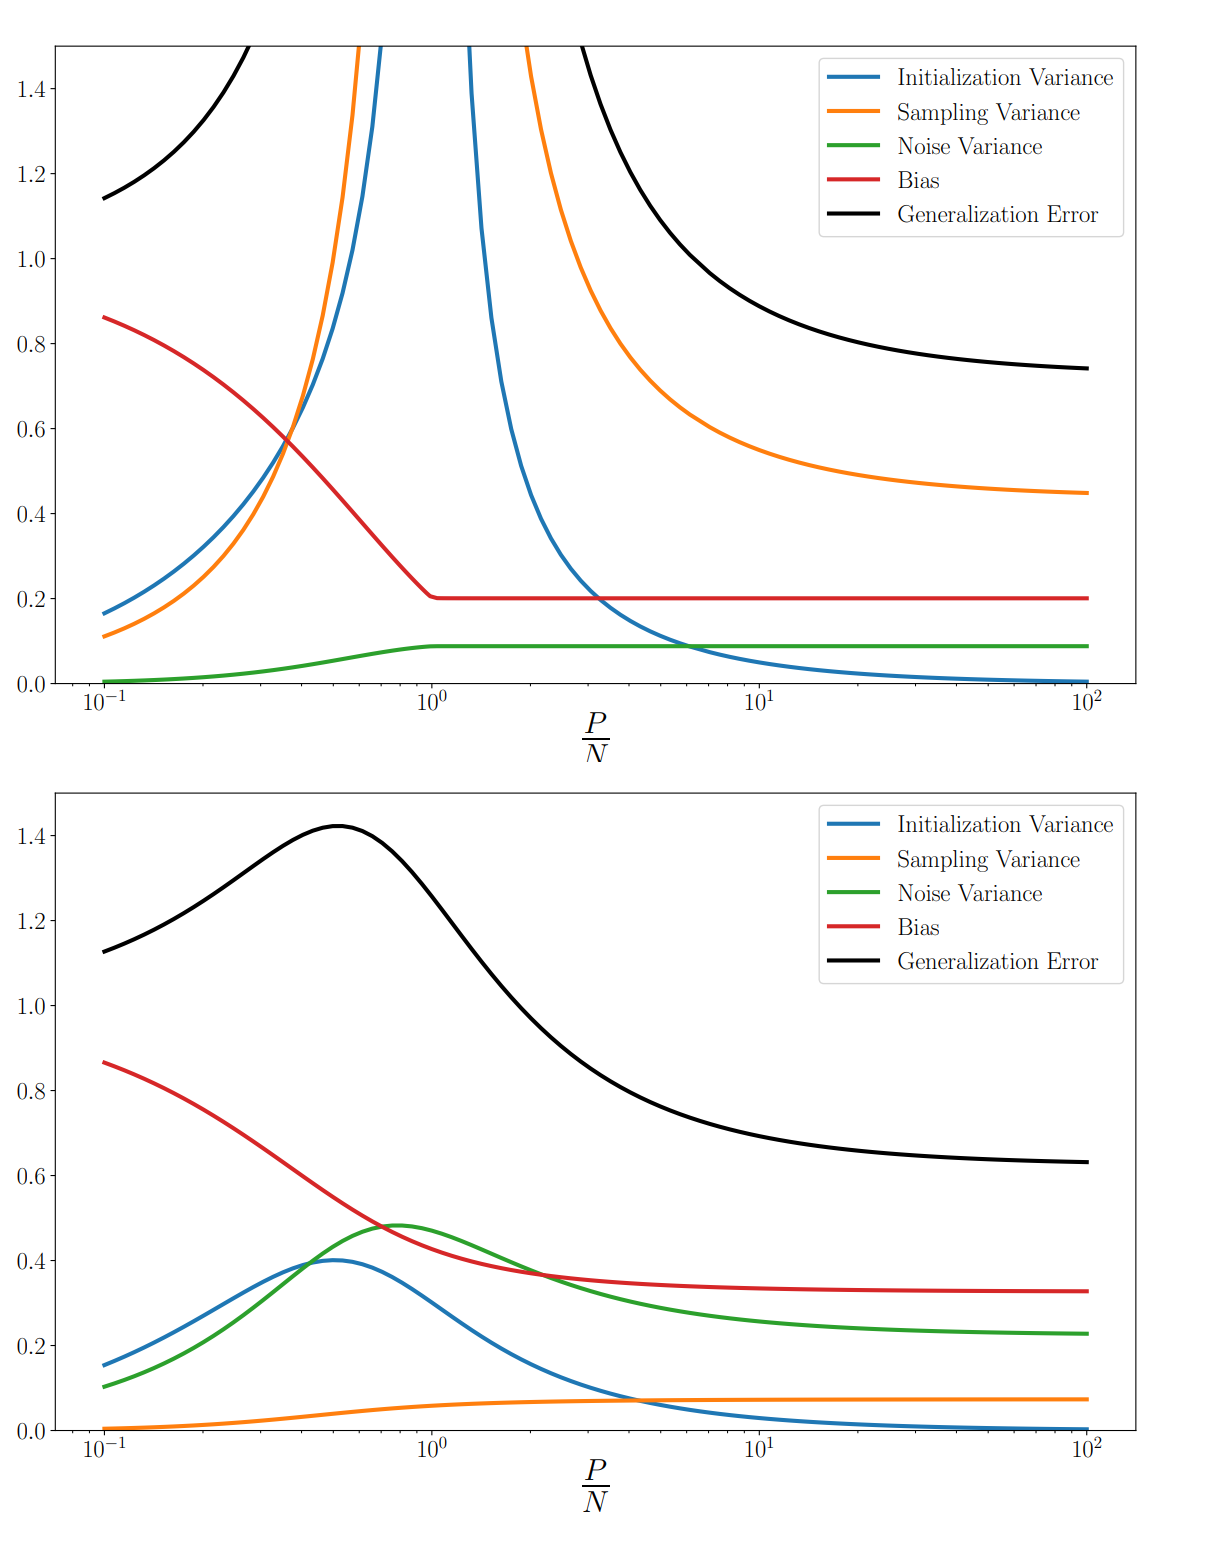
\includegraphics[scale=0.45]{Abschlussarbeit_2021/LaTeX/images/variances_ascoli.PNG}
\caption{Plot from \cite{pmlr-v119-d-ascoli20a}. In the upper plot the model was only weakly regulated. In the lower plot, however, it was regulated more strongly. The ratio $\frac{P}{N}$ describes the number of features in relation to the size of the data set. If this term is 1, the data can be interpolated perfectly \cite{belkin}. The analysis was performed with an RF model, which was first presented in \cite{RF-model}}
\label{fig:varianz_ascoli}
\end{figure}


\begin{figure}[!htp]
\centering
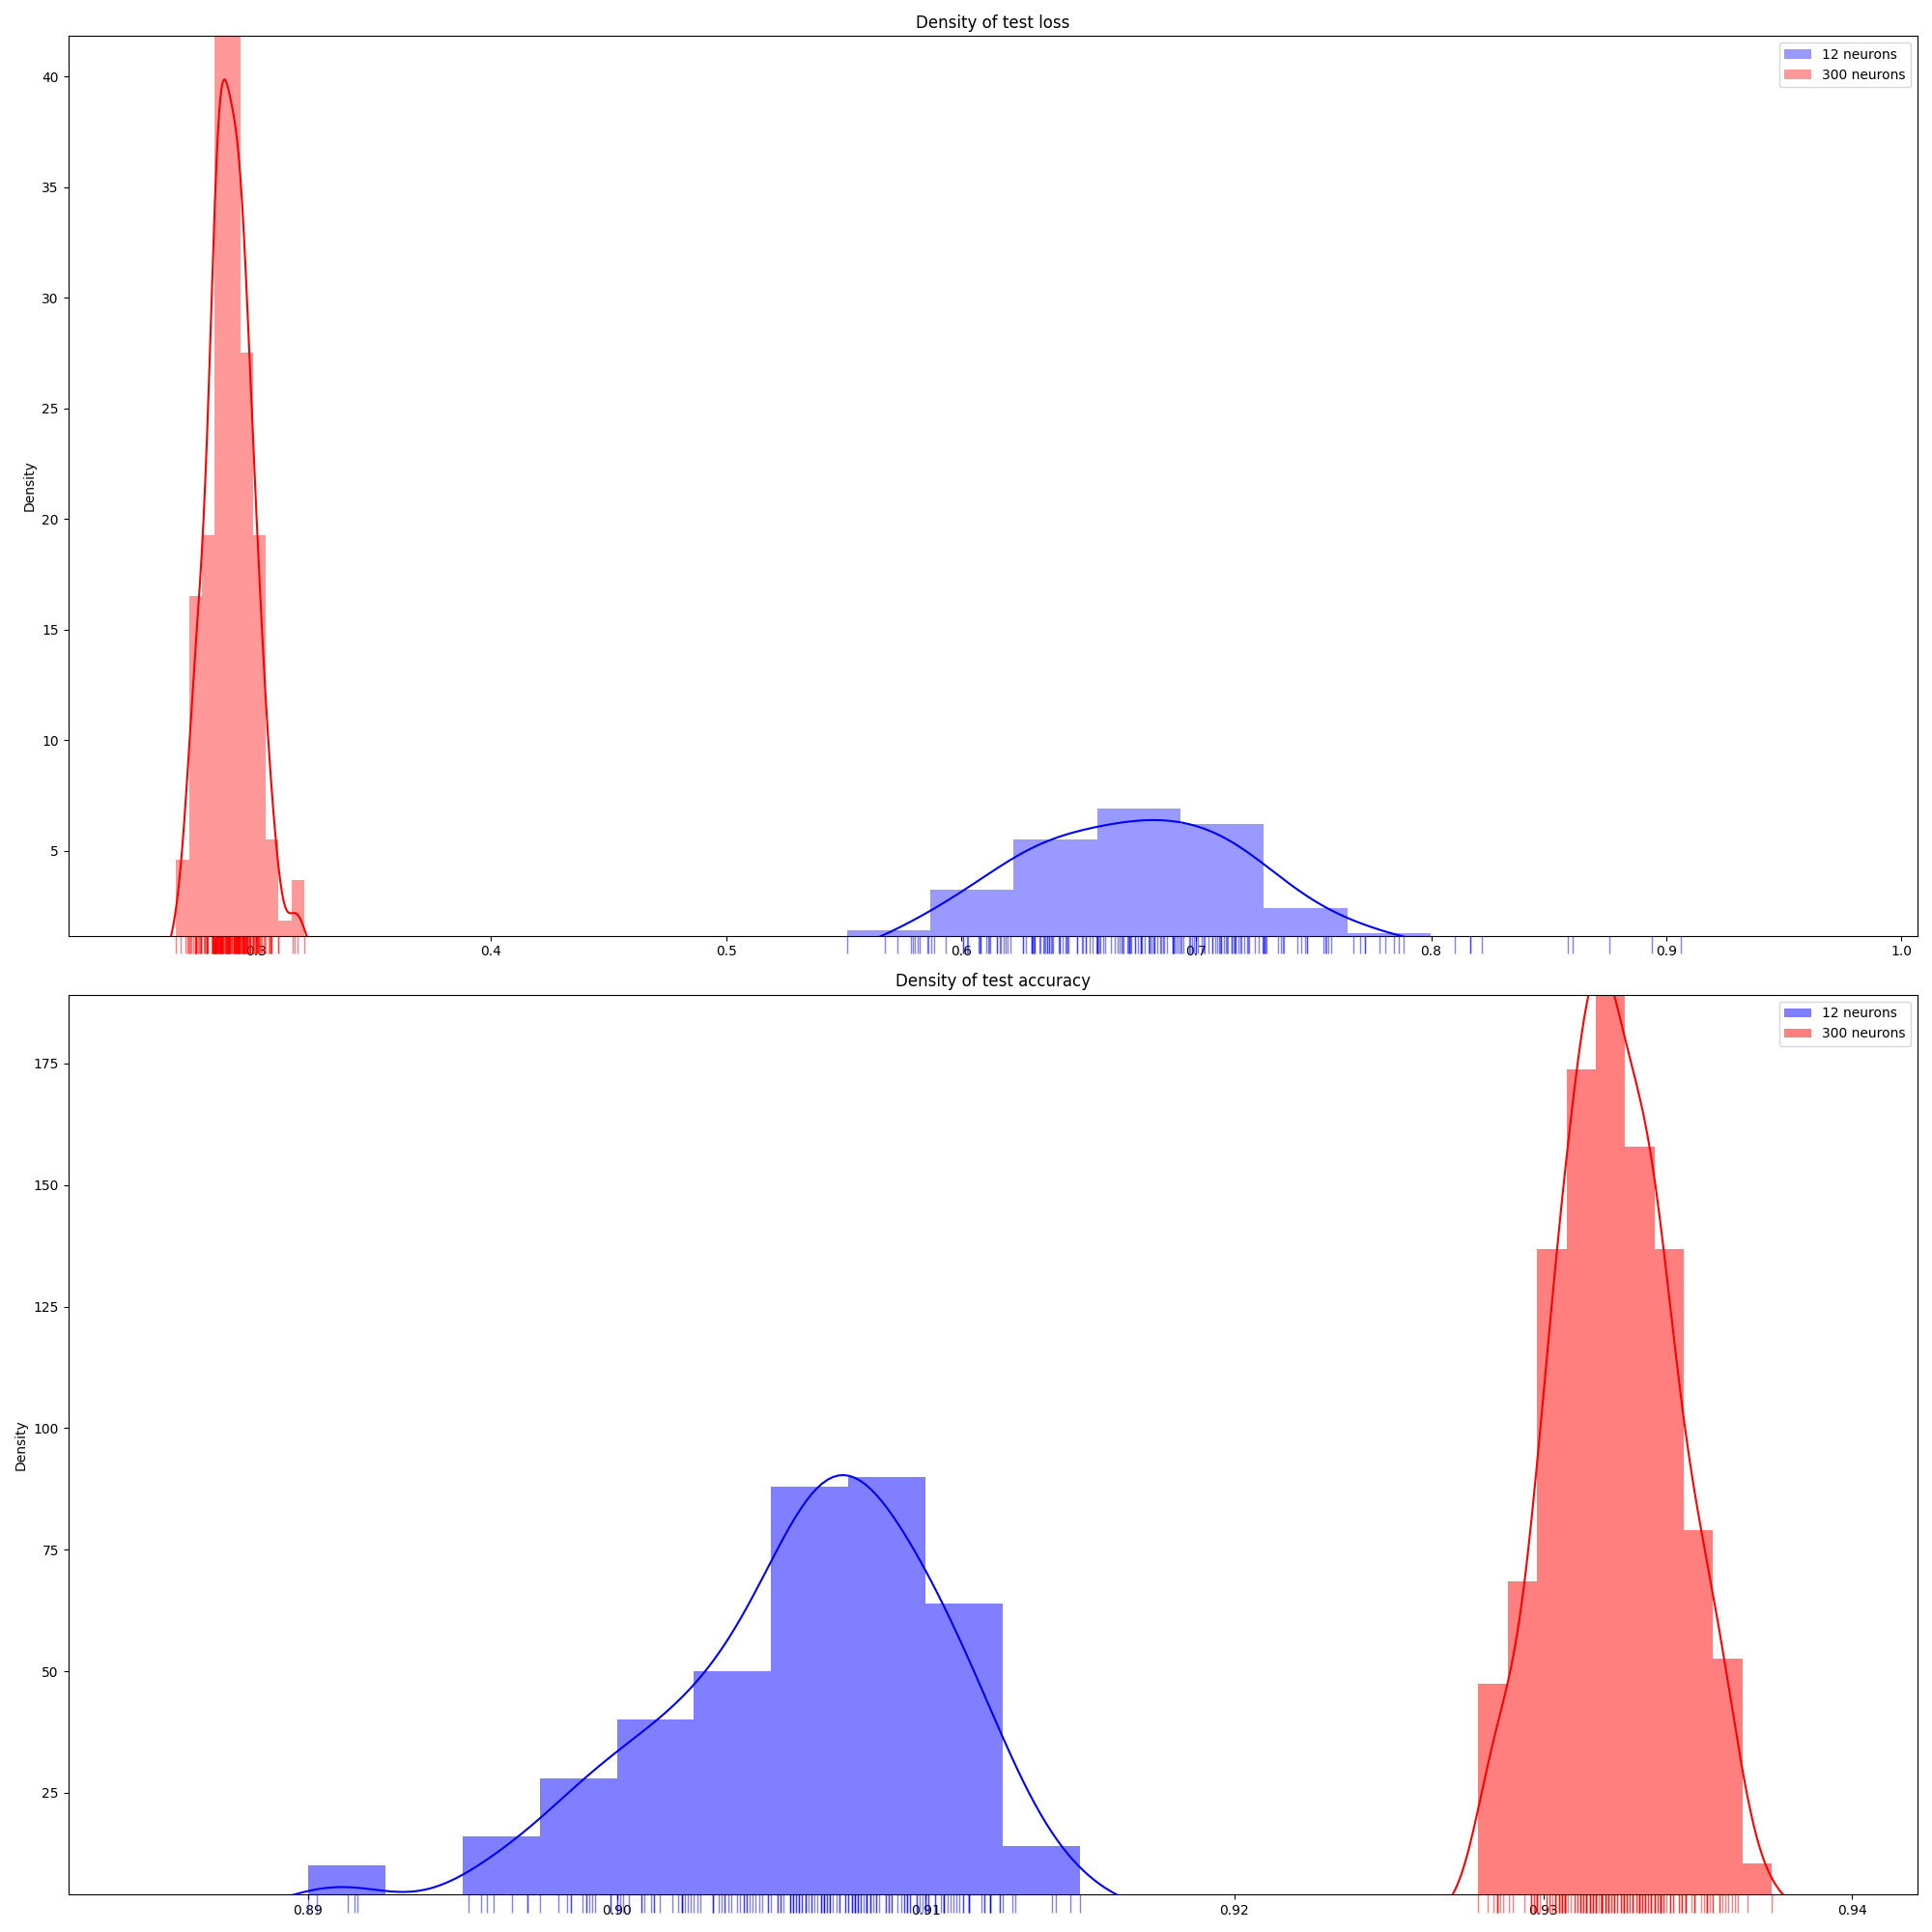
\includegraphics[scale=0.3]{Abschlussarbeit_2021/LaTeX/images/varianz_test.png}
\caption{Variance of test loss (top) and variance of test accuracy (bottom) experimentally generated with the MNIST dataset. In blue a network of 12 neurons and in red a network of 300 neurons.
In total, the networks were trained 200 times to obtain the data set.}
\label{varianz_mnsit}
\end{figure}

\newpage






\subsubsection{Exploration at inizialization and weight-clustering}
\label{weight-cluster}

Another interesting effect that can occur with weakly overparameterized networks is called "Insufficient Exploration" \cite{pmlr-v97-brutzkus19b}. \\
 Depending on the initialization of the weights, it can happen that even if there are enough neurons so that training data should be learned perfectly, a local minimum is found by the optimization algorithm, which still leaves the network with a non zero training error. So at least a few weight are not converging to where it should for better performance during the training process. this is called insufficient exploration. The effect was shown in \cite{pmlr-v97-brutzkus19b}\\
In \ref{fig:XOR-problem} this effect can be observed. In the Experiment a Model tries to learn the XOR-function. Here it can be seen that with few weight vectors an optimal minimum may not be found. With more weights it is much less likely that "Insufficient Exploration" occurs, because depending on the initialization of the weight vectors they converge to a certain cluster \cite{pmlr-v97-brutzkus19b}.Insufficient exploration can occur even with zero training loss \ref{fig:brutzkus19b}. Thus, the effect has a strong influence on overparameterized networks.

\begin{figure}[!htp]
\centering
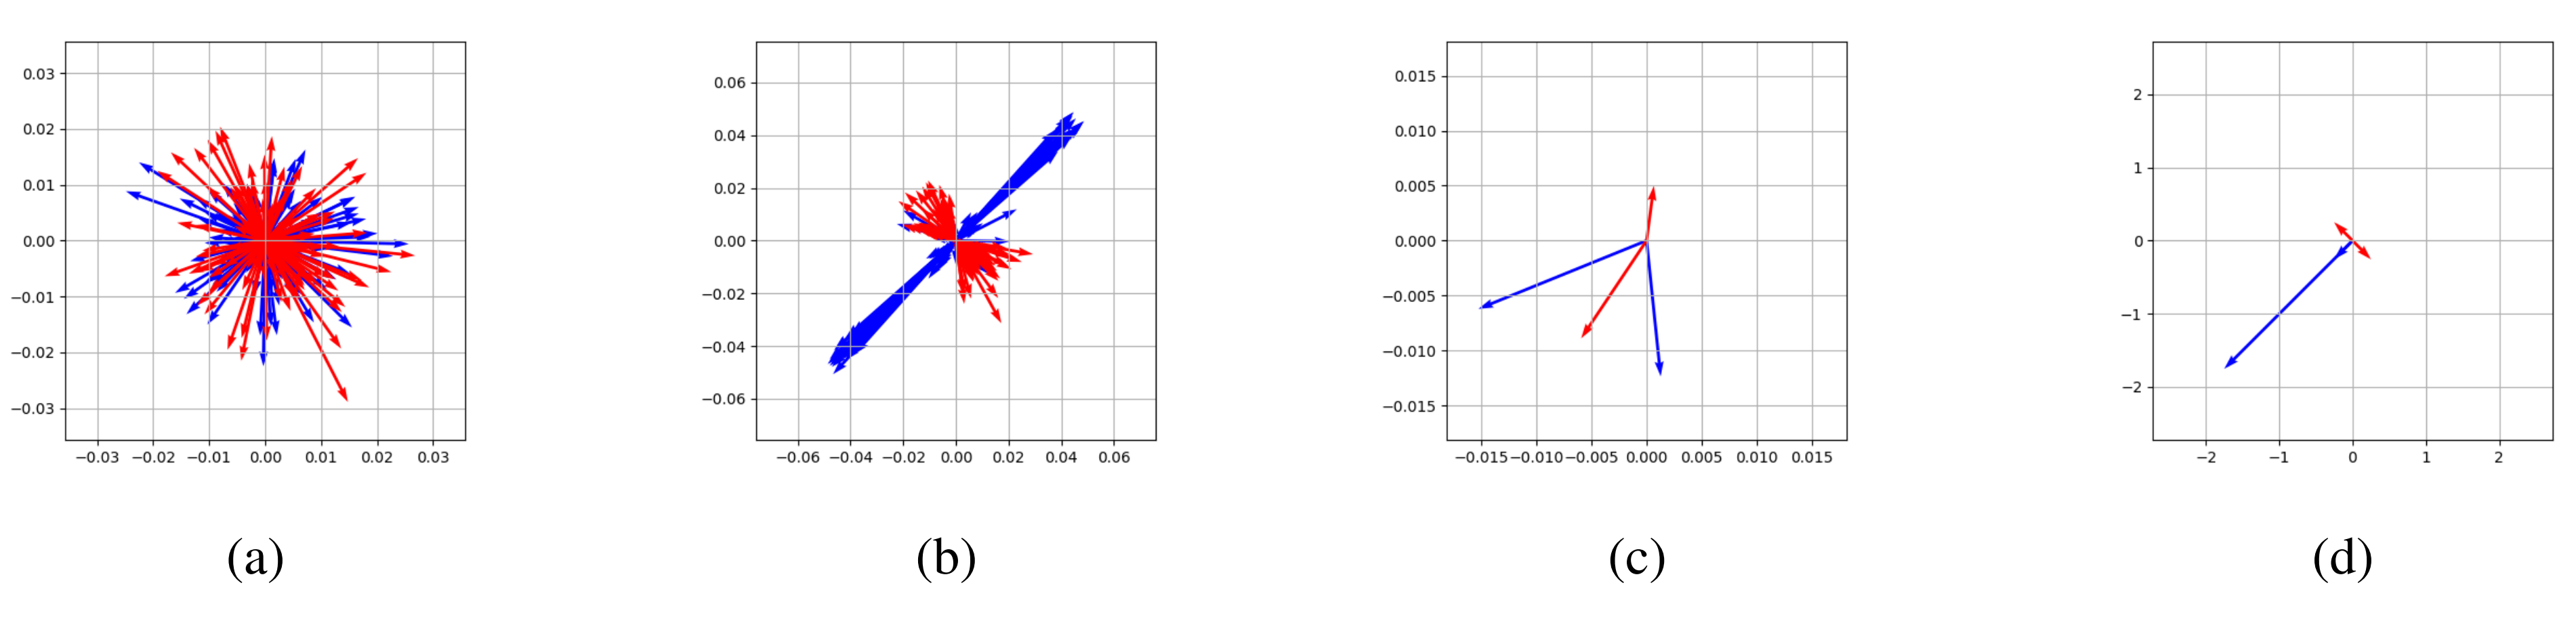
\includegraphics[scale=0.2]{Abschlussarbeit_2021/LaTeX/images/XORD.PNG}
\caption{in $(a)$ and $(c)$ weight vectors before training are shown. in $(a)$ a total of $100$ weight vectors are used for training. in $(c)$ there are $2$ weight vectors, which would be sufficient for the problem with optimal weighting. The weight vectors after training can be seen in $(b)$ and $(d)$. At $(d)$ an under-exploration can be observed \cite{pmlr-v97-brutzkus19b}.}
\label{fig:XOR-problem}
\end{figure}




Another interesting observation which also can be observed in \ref{fig:XOR-problem} is weight clustering. Weight clustering means that the weight vectors of a neural network form clusters during training. In the paper this was also empirically shown for larger Networks. Using the MNIST data set, it was shown that the channels of a convolutional network cluster \cite{pmlr-v97-brutzkus19b}. For this purpose a three layer network is constructed, which has as first layer a convolutional layer with $3 \times 3$ filters. The number of channels are changed in this layer. The second layer is a maxpooling layer and the third layer is a fully connected layer.\\
In Figure \ref{fig:brutzkus19b} (a), it can be clearly observed that the training causes clusters to form and the weight vectors to move closer together. It is also shown that initializing small networks with clusters of trained larger networks results in significantly better performance and generalization than using random weights for initialization. This can be observed in Figure \ref{fig:brutzkus19b} (b). For the small network four channels were used (red and blue) for the large network (green) from which the initialization emerges, $120$ channels were used. 
  



\begin{figure}[!htp]
\centering
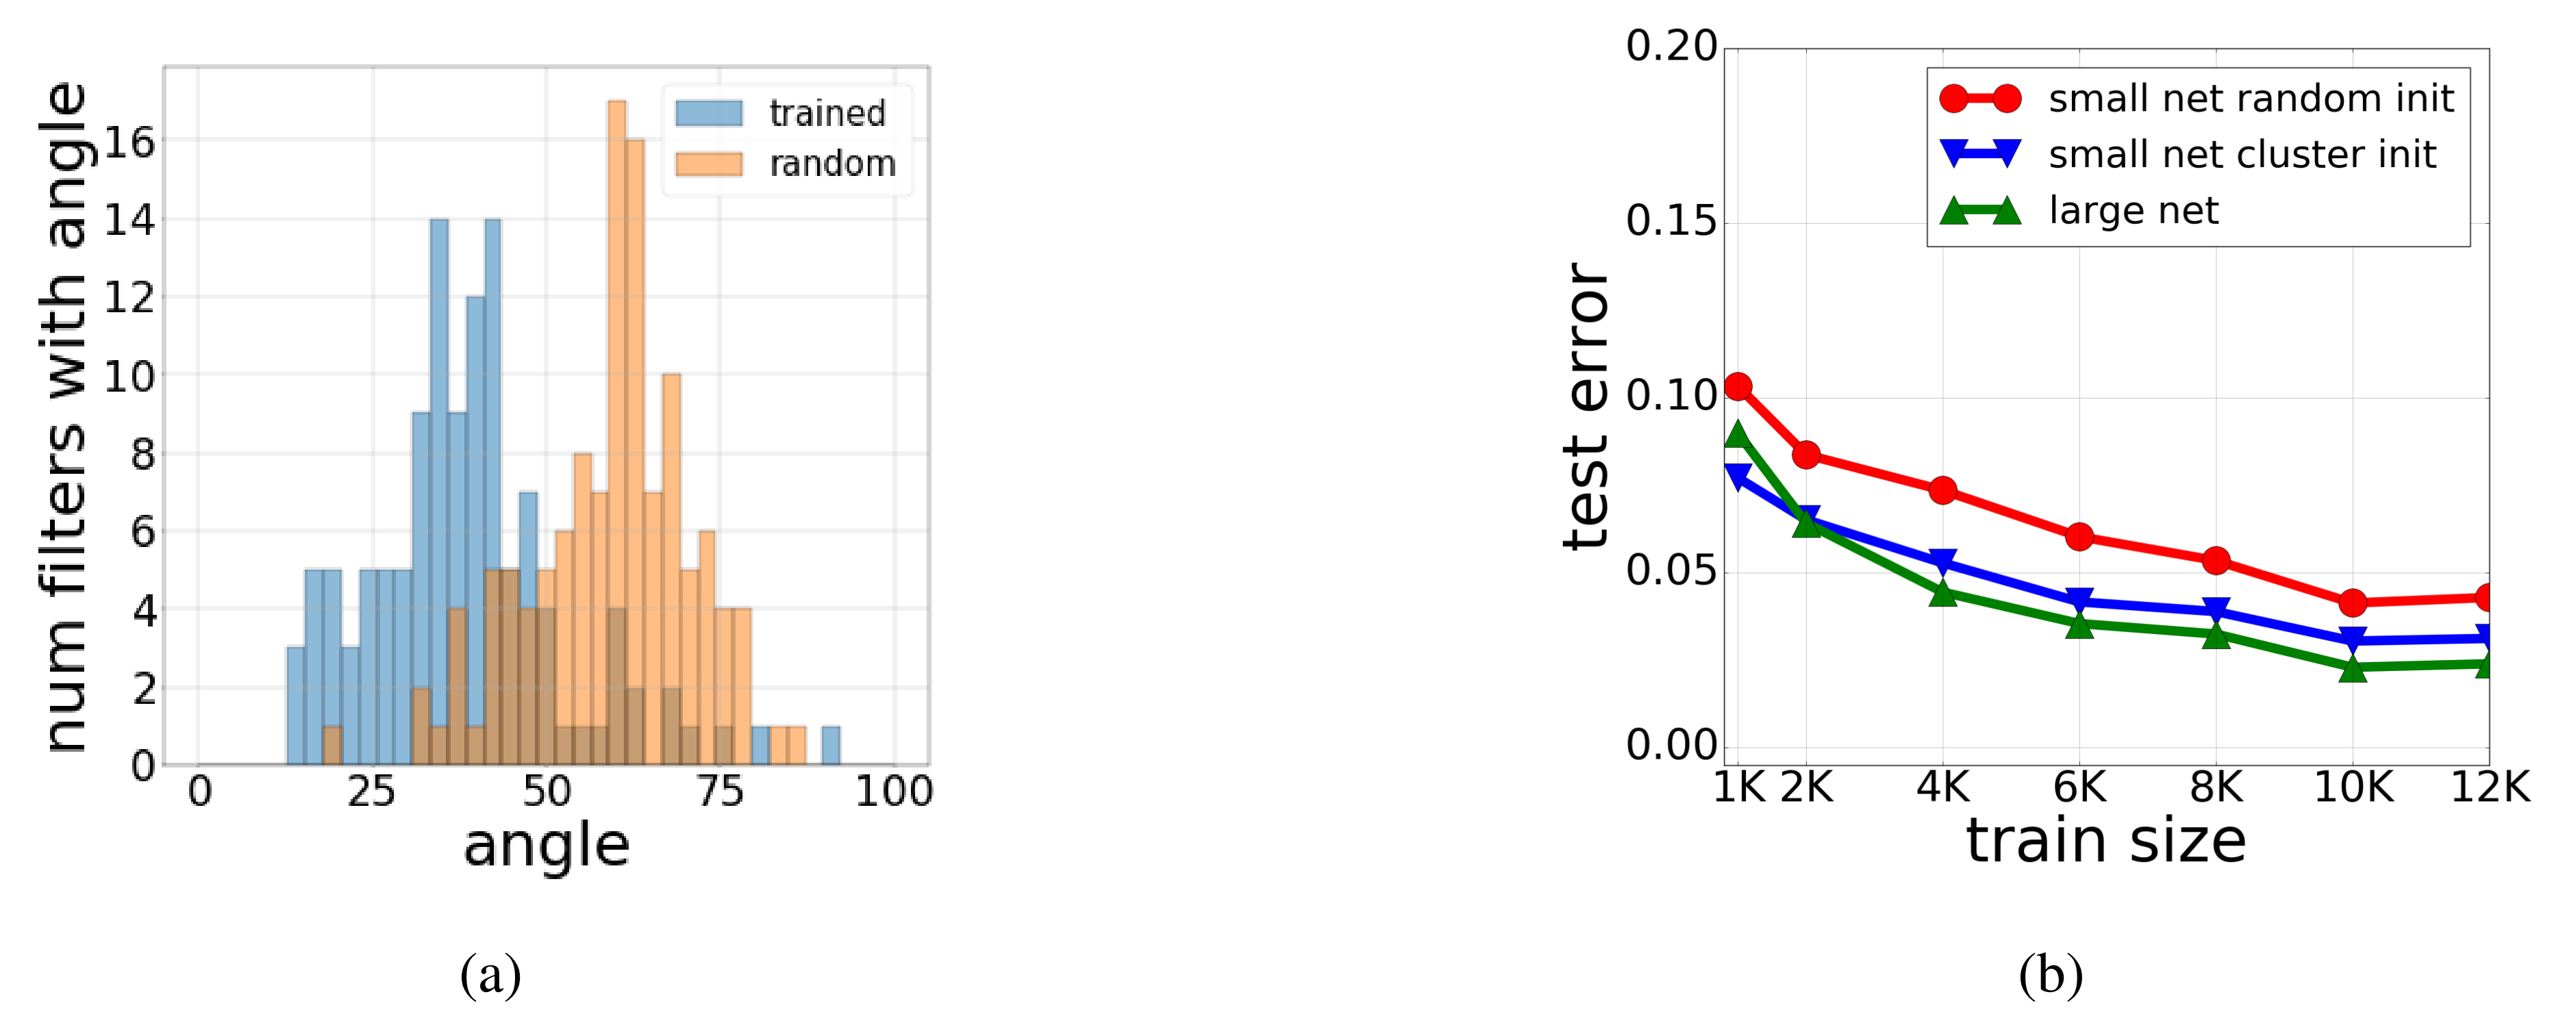
\includegraphics[scale=0.2]{Abschlussarbeit_2021/LaTeX/images/clustering.PNG}
\caption{ Graphic from \cite{pmlr-v97-brutzkus19b}. 
(a) Distribution of angle to closest center in trained and random networks. (b) The plot
shows the test error of the small network ($4$ channels) with standard training (red), the small network that uses clusters from the large network (blue), and the large network ($120$ channels) with standard training (green)}
\label{fig:brutzkus19b}
\end{figure}





\newpage
\subsubsection{The impact of the loss landscape}

In this section, the focus will be on the loss landscape. The local minimum found by the optimizer is strongly dependent on the shape of the loss landscape. A very hilly and uneven landscape could cause SGD to run into unfavorable minima during the training process.
So it would be interesting to see what would happen if you artificially smoothed this loss landscape. Thus, SGD would no longer be in an unfavorable local minimum.  \\
In order to test the influence of the loss landscape with different size networks, another experiment will be conducted. Here, the loss landscape of different sized networks as in \ref{model equation} $(1 \leq H \leq 60)$ is to be smoothed and then the performance evaluated. 
To smoothen the loss landscape, the so-called SAM-optimizer\footnote{ For more information about the optimizer, see sharpness aware minimization for efficiently improving generalization \cite{sam_optimizer}
} (sharpness aware minimizer) is used.



\begin{figure}[!htp]
\centering
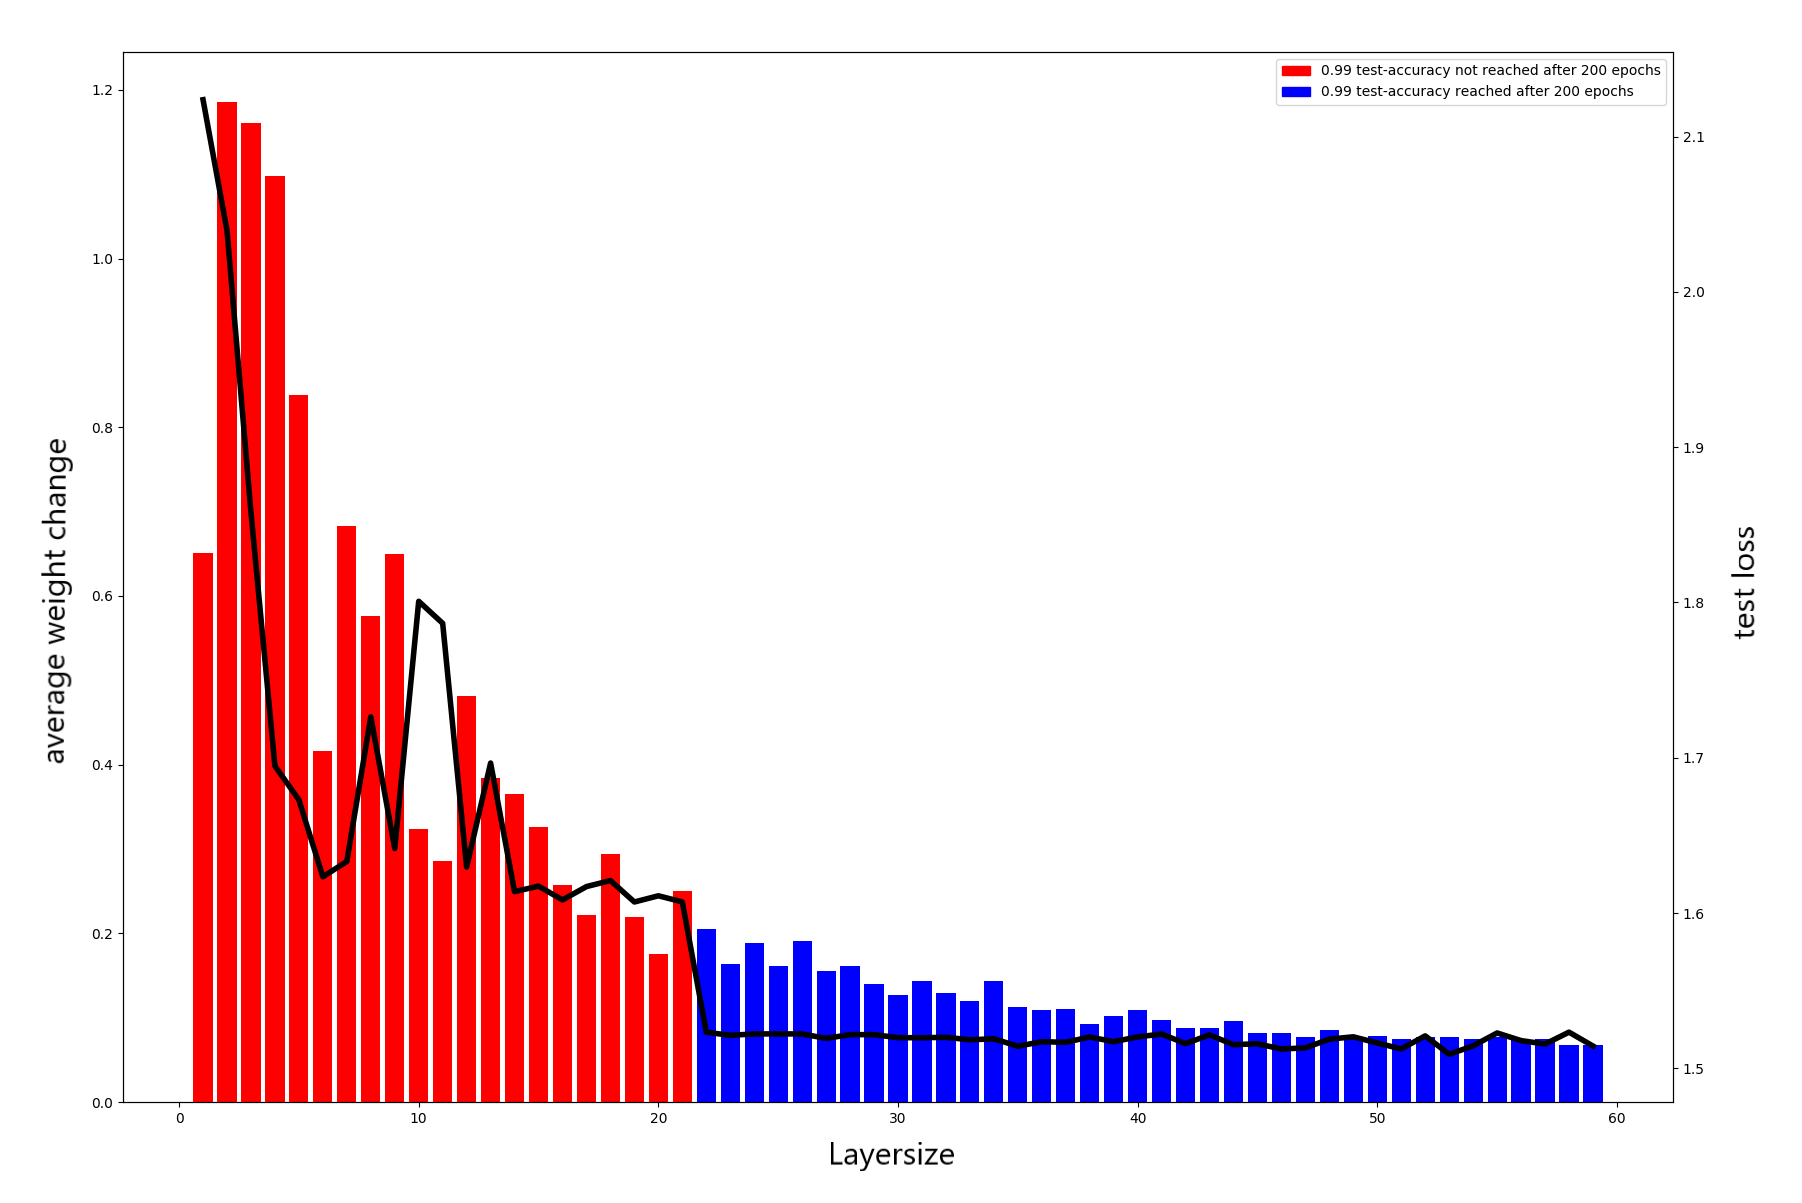
\includegraphics[scale=0.3]{Abschlussarbeit_2021/LaTeX/images/sam_edited.bmp.png}
\caption{Test loss and average weight change as a function of network size. The SAM-optimizer was used for training\cite{sam_optimizer}. A smoothing factor of $\rho = 0.05$ was used. The data set is a subset of MNIST with $15000$ samples.}
\label{fig:sam}
\end{figure}

In Figure \ref{fig:sam} the result of the experiment can be observed. Double Descent is still visible. However, it is interesting to note that above a certain network size $(H = 22)$ the minima found almost all provide for equally good performance. This is also the point from where the training accuracy is always above $0.99$. The addition of parameters does not provide a better generalization. So smoothing the loss-landscape can change the behavior of Double Descent in the overparameterized region. \\
Increasing the smoothing factor $\rho$ provides for the blunting of the peak at the interpolation threshold\footnote{The word interpolation threshold might be a bit misleading here. Finally, it is clear from Figure \ref{fig:sam} that the training data is not yet perfectly interpolated, as not even a training accuracy of $99\%$ has been achieved. However, the $H$ at which the peak can be seen is the same as in \ref{avg_weightchange}, where the same data set was used only without smoothing. So the sample size is identical in both experiments. However, the smoothing also ensures that the minima found, which would previously have interpolated the data perfectly, is also smoothed and thus a regularization happens.}
and earlier constant behavior of the test loss (in \ref{fig:sam} at $H=22$). This can be seen in the appendix \ref{sam_extension}. 




\newpage
\subsection{Possible explanations} 
    \label{possible_explanations}
    
    
The previous section has given a good overview of the behavior of overparameterized networks. In this subsection possible explanations for this phenomenon and assumptions for the occurrence will be given and linked to the findings from the observations of Chapter \ref{experimental_part} and Section \ref{over-p-regime}. The answer to the question why bigger and bigger networks perform better and better will be explored here. \\
It must be clearly stated that the explanations are only conjectures supported by the observations made earlier. All explanations for the Slope of the double-descent risk curve after the interpolation threshold are only described here but not proven. This is merely a conjecture. For future work it would be interesting to go deeper into the matter and to do more research.  \\


\subsubsection{Regularization in large networks}

In Figure \ref{avg_weightchange} we have already shown empirically that the average weight change $\bar{w}$ decreases with higher model complexity. This is due to the fact that a large neural network with a large number of parameters makes it much easier to find a minimum that interpolates the training data. This can also be observed in Figure \ref{avg_weightchange}. One reason for this is that with a large number of parameters, significantly more minima can be found that perfectly interpolate the training data. A nice example can be found in \cite{double_descent_2021_splines}. \\
For large networks, significantly fewer epochs are needed to find a suitable minimum. Accordingly, weights do not have to be adjusted too extremely. A more uniform weight adjustment would thus be possible. Also, of course, minor changes must be made to the individual weights to compensate for the error in the loss function. For example, for a typical optimization problem of a model with $m$ layers with $H$ neurons each and one output neuron using the mean squared error. Then the error function, which we want to minimize is given by,
$$
E(x) = (y^* - y)^2 = (y^* - \sum_{ i= 1}^{H} w_{i}^{(m)})^2
$$
Where $y^*$ is the true desired value and $y$ is the output of the model. It is easy to see that for large $H$ the single weight has less and less influence on the error. The weight adjustment after the backpropagation step is correspondingly lower. \\
Thus, also the terms $\frac{1}{|W|}\sum_{w \in W} |w| $ and especially also $\frac{1}{|W|}\sum_{w \in W} \lVert w \rVert_2^2$ are significantly lower for large networks. The latter especially, since the weight distribution does not vary so much for large $H$. This was shown in Figure \ref{density_weights}. Often the terms just mentioned are intentionally kept small when training. This is called $L1$ or $L2$ regularization \cite{regularization_L1_L2}. 
The error function $E^*(x)$ with regularization is then given by,
    $$
    \text{with $L1$ Regularization:  }  E^*(x) = E(x) + \lambda \sum_{w \in W} |w| 
    $$
    $$
    \text{with $L2$ Regularization:  }  E^*(x) = E(x) + \lambda \sum_{w \in W} \lVert w \rVert_2^2
    $$

where $E(x)$ is the old error function without penalty term at the end, which is regulated by $\lambda$. To keep the error small here, the model tries to learn the training data and not to let the weights become too large. \\
So it would be a plausible theory that the network size implicitly behaves as a regularizer \cite{A_least_squre_study}, which then would lead to a simpler and smoother output function as observed in chapter \ref{RFF}. This would also explain why the variance of the learned function decreases with large models. The implicit regularization would prevent too large fluctuations to occur. The same effect has $L1$ and $L2$ regularization in neural networks. They prevent overfitting \cite{regularization_L1_L2}, which occurs as in chapter \ref{bias_variance} described, with high variance of the learned function.\\
\cite{l2_regularization_double_descent} shows empirically that using L2 regularization with a good choice of $\lambda$ as regularization factor the peak of the double descent curve disappears. Then there is a monotonic decay of the test loss. This supports the assumption that the shrinking variance in the weight distribution has an influence on the regularization and thus also on the generalization.
%%%%%%%%%%%%%
%%%%%%%%%%%%%
%%%TOWRITE%%%%
%%%%%%%%%%%%%
%%%%%%%%%%%%%




\subsubsection{Lottery ticket hypothesis}
Another explanation, which could also be a possible explanation for the second decrease of the risk curve, is the so-called lottery ticket hypothesis \cite{understanding_double_ticket}.
This hypothesis was first formulated in the paper by Frankle and Carbin \cite{lottery_ticket} and states the following: %%Quote%% 
\\
\begin{quote}
A randomly-initialized, dense neural network contains a subnetwork that is initialized such that—when trained in isolation—it can match the test accuracy of the
original network after training for at most the same number of iterations."\cite{lottery_ticket}
\end{quote}

A subnetwork here means a subgraph of the graph of the neural network. In other words, a subset of edges that are present in the neural network.  
So if there are $n$ weights, there exist $2^n$ subgraphs, since $|\mathcal{P}(E(G))| = 2^{|E(G)|}$, Where $E(G)$ are the edges of the Graph of the Network. The number of subgraphs increases exponentially with the addition of neurons. In the paper, the possible existence of the hypothesis was shown empirically. \\
First, a large network $N = (V,E)$ was trained. After the training process, a subnetwork
$N^{'} =  (V^{'},E^{'})\subset N$ was selected, a so called winning ticket \cite{lottery_ticket}. When selecting the subnetwork, care was taken to ensure that it contained weights $E{'}$ that also underwent some change during the training process. \\
After that $N$ was reinitialized and trained under two different circumstances. First all weights $E^* = E \setminus E^{'}, V^* = V \setminus V^{'}$ which are not contained in the subnetwork were reset to their original initialization. In the second training session all weights $E,V$ were randomly initialized again. It was found that the first variant found a minimum significantly faster, i.e. SGD converges significantly faster. And that the initialization with random new weights generalizes worse \cite{lottery_ticket}. \\
Interestingly we have made the same observations in figure \ref{avg_weightchange}. regarding small and large networks. Larger models find a minimum faster  and generalize better than small models. So similar to the models with partially learned initial weights and random weights.\\
An obvious hypothesis would be that large networks, which due to their large number of weights also contain significantly more subnetworks, have a higher probability of containing a so-called winning ticket. It is therefore more likely that SGD finds a fast minimum with the help of an already initialized subnetwork, which leads to a good generalization. \\
Since the number of subnetworks increases exponentially, SGD would have significantly more choice. A large network has therefore bought more tickets for the lottery. Small networks, on the other hand, rely on good initialization. \\
In figure \ref{density_weights}, it can also be observed from the density function of the weight changes (right) that more and more weights do not change at all or at least only a tiny amount with increasing model size as a result of the training process. This would argue for a focus on subnetworks. Just like the ever decreasing variance of the learned weights. This could speak for more and more favorable initialized subnetworks. Even if the lottery ticket hypothesis is only a hypothesis, the experiment conducted in the paper already provides insights into this possible explanation of double descent.
It would be also interesting to link this hypothesis with the finding of weight clustering described in \ref{weight-cluster}. Again, a smaller network with learned weights from a much larger network could perform better.
Even so, many points are unclear. How does SGD select these subnetworks?  And how do few weight changes succeed in taking profits from these subnetworks? What the reason for double descent, many questions which still need to be answered.



\newpage


%%%%%%%%%%%%%%%%%%%%%%%%%%%%%%%%%%%%%%%%
%%%%%%%%%%%%%%%%%%%%%%%%%%%%%%%%%%%%%%%%
%%%%%%%%%%%%%%%%%%%%%%%%%%%%%%%%%%%%%%%%%







\section{Discussion}
    \label{Discussion}

In Chapter \ref{experimental_part} it was noticed that the height of the peak at the interpolation threshold which is to be found at the point where the model is able to interpolate the training data is strongly dependent on factors that lead to overfitting. This could be observed at high number of epochs, high amount of noise and high learning rate. (to be seen in figure \ref{fig:epochs_double_descent}, figure \ref{fig:Label_noise_on_double_descent} , figure \ref{fig:learning_rates_double_descent}). All three factors provide strongly different functions when the training data is to be interpolated. If the number of epochs is high or the learning rate is high, weights are changed more. So there may be high variances with respect to the functions learned. With high noise, noisy data points are also interpolated. The result is also overfitting. In the case of noise, this can also be observed in the overparameterized range (figure \ref{fig:Label_noise_on_double_descent}). Thus, we have a high variance. The resulting high peak is thus explained by the bias variance trade-off described in chapter \ref{bias_variance}. The behavior to the left of the interpolation threshold is therefore predictable and traceable, among other things with the worked out equation \ref{bias_variance_eq} concerning quadratic error, bias and variance. \\
The situation is somewhat different on the right side of the interpolation threshold. From here on, the double descent curve decreases monotonously. Under certain conditions, a learned function can even perform better on a test data set than a learned function that does not interpolate the data. This can be observed in figure \ref{double_descent_vanilla}. However, this does not necessarily have to be the case (can be seen in figure \ref{fig:double_descent_wine}). \\
An idea why the generalization curve decreases monotonously is given by the experiments with random fourier features in \ref{RFF}. Here it can be observed that models with more parameters learn simple and smoother functions (to be seen in figure \ref{fig:1d_rff}, figure \ref{3d_RFF}, figure \ref{decision_RFF}). So models with many parameters get a sense of the data. This is called inductive bias \cite{wikipedia_inductiv_bias}. This means the model gets better and better in generalizing the training data with increasing number of parameters.\\
Further observations were then made on the behavior of overparameterized networks. It has been empirically shown that SGD with increased number of parameters finds a minimum that interpolates the training data much faster. This can be done by taking a look at the number of epochs needed (to be seen in figure \ref{avg_weightchange}). The average change of a weight is significantly lower for highly overparameterized networks (also to be seen in figure \ref{avg_weightchange}). It can therefore be assumed that a network with many parameters will find it much easier to interpolate the training data. Which is also an expected finding. Even if the loss-landscape was intentionally smoothed as in \ref{fig:sam}, a training accuracy of over 0.99 can still be achieved.\\
It has also been shown empirically that the variance of between-learned functions decreases with increased number of parameters (seen in figure \ref{varianz_mnsit}). This can also be due to the fact that interpolating functions are found faster and thus not too large differences between learned functions can occur. We also have seen in chapter \ref{RFF} that learned functions become smoother under the constraint that they have to interpolate the training data points. This also causes a decrease of the variance (also to be seen in figure \ref{fig:1d_rff}, figure \ref{3d_RFF}, figure \ref{decision_RFF}). Equation \ref{bias_variance_eq}, which describes the relationship between generalization, bias, and variance, can also be used to explain the behavior in the overparameterized region. Since the bias is very small after the interpolation threshold, the variance must be monotonically decreasing in the overparameterized regime. This is confirmed by our observations. If there is a lot of noise in the data set, the variance falls off more slowly. see  figure \ref{fig:Label_noise_on_double_descent}. \\
In section \ref{possible_explanations} possible explanations for the drop of the curve after the interplationthreshold were given.  The first section dealt with the self-regulating effect that neural networks develop when the number of parameters is large. This effect is strongly related to the decreasing variance and also ensures that networks develop an inductive bias for their training data. This in turn leads to better performance. A possible reason for this self-regulating effect could be the smaller change of the weights(see figure \ref{avg_weightchange}) with increased parametersize. Similar to $L1$-regularization or $L2$-regularization where a penalty term is used to ensure that weights do not become too large. \\
As a second possible explanation, the "winning lottery ticket hypothesis" was listed. This states that during the training process subnetworks are selected which already show good convergence behavior with the initialization. Thus, simple and good minima can be found. This could be related to the found in figure \ref{avg_weightchange}. Larger networks find desired minima faster and easier. As the number of parameters increases, the number of existing subnetworks increases exponentially. So there is more choice during the training process. This also relates to the fact, that rich models will have a lot more possible minima which interpolate the training data. A connection can also be made to section \ref{weight-cluster}. Here it was also described that weight vectors cluster in the overparameterized section. If these clusters found by large networks are inizialized to smaller networks, very good performance can still be achieved.\\
In general, it can be said that the behavior of the curve is comprehensible for both the underparameterized range and the overparameterized range.  Even if for the modern regime an exact and detailed explanation is still waiting. Now we can put together our two components, which we have worked out in this chapter, and get a deeper understanding of the double descent risk curve. 




%TODO bring in the variance and discuss it. Link it to the RFF funktions
%TODO sam optimizer 
%Todo possible explanations 
    
    
    
    

\chapter{Training Models under the Consideration of Double Descend}
\label{train_dd}

The last chapter of the thesis is about the practical application of double-descend. An important and simple question, is first of all how to construct and train a model so that it achieves the best possible performance i.e. archives the best possible generalization of the data. Depending on the application, there are already many tricks for training the models to get the best performance. By taking this phenomenon into account, many performance losses can be avoided. In this chapter, a small analysis will be made on how generalization can be improved by taking double descent into account.\\
\\
\section{The Impact of the Data set}
    \label{The Impact of the Dataset}
A simple thought that seems immediately logical would be to simply make the model as large as possible and then train it until the training accuracy is 100\%. Under certain circumstances this is a good idea. In chapter \ref{experimental_part} we saw that, there can be a point in the overparameterized regime from which the performance is always better than the sweet spot in the underparameterized regime \ref{double_descent_vanilla}. However, it can also be observed in chapter \ref{experimental_part} in Figure \ref{fig:double_descent_wine} that interpolating all training data does not necessarily produce the best performance. Also in chapter \ref{RFF}, for example in figure \ref{fig:1d_rff} , a simple straight $g$ with $g(x) = x = f^*(x)$ the above titled "true function" would be the best possible regression function. For Figure \ref{3d_RFF} and \ref{decision_RFF} the same applies. In Figure \ref{decision_RFF}, for example, a model which colors the decision space red for $x \leq 0$ and blue for $x > 0$ would be on average the optimal model. A perfect interpolation of the intercepted points is not necessarily beneficial here.   
%%%
\begin{figure}[!htp]
\centering
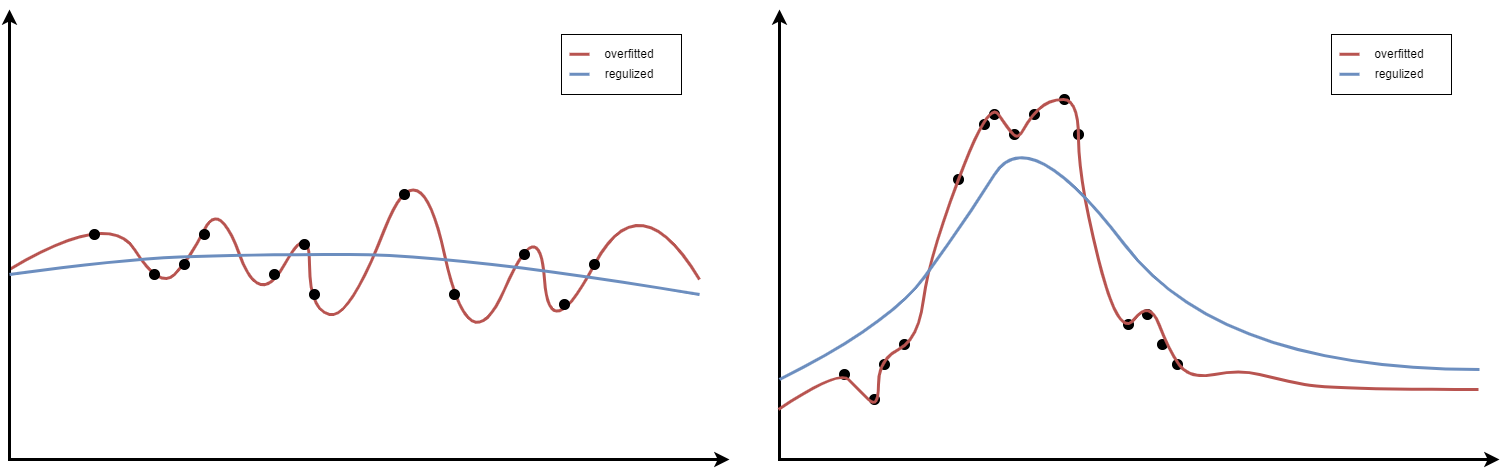
\includegraphics[width= 1\linewidth]{Abschlussarbeit_2021/LaTeX/images/good_baad_to_overfitt.drawio (2).png}
\caption{On the left side, the highly regulated function is to be preferred. On the right side, the perfectly interpolating function performs better. It is also often a question of how much regularization is beneficial}
\end{figure}
%%%
\\
Furthermore the second question that must then be asked is: Can we always reach this said point? We also observed in Chapter 2 that as the size of the data set increases, the underparameterized regime becomes larger and larger and the interpolation threshold shifts further and further to the right (see figure \ref{fig:sample_size_double_descent}). Thus, significantly more variables are needed to memorize larger and larger data sets. Of course, this also shifts the point in the overparameterized regime, from which a better performance is achieved. If we follow the observations from Chapter \ref{experimental_part}, we find that for the MNIST data set, the interpolation threshold, given by the amount of neurons in the hidden layer, can be roughly represented as,
$$
H \leq \frac{n}{1000} 
$$
Where  $n$ is the amount of Data we train with. However the amount of epochs we train also has an impact on the position of the interpolation threshold. Note, that the amount of weights we train depends on the size of the one hidden layer $H$, the input dimension $d = 28\cdot28$ and the output dimension $K = 10$. Therefore the total amount of weights and biases $W$ in the experiment is given by,
$$
W_{MNIST}(H) = (d+1)\cdot H + (H+1) \cdot K
$$
The article by Makhail Belkin gives for the same experiment the number of weights needed with $n\cdot K$ \cite{belkin}. \\
One can imagine that for a more complex problem with a lot of data, such as an image recognition problem, for example IMAGENET, the number of required parameters must be very high. The current record for the largest model is held by the PTD-3 with 175 billion trainable parameters\cite{Artificial_neural_network}. IMAGENET has 14 million images pread across 20,000 different classes \cite{wikipedia_Machine_learning}. With Belkin's formula, you would need for the interpolation threshold alone,
$$
n \cdot K = 14 \cdot 10^{6} \cdot 2 \cdot 10^{4} = 28 \cdot 10^{10}
$$
So 280 billion parameters would be needed. It would probably be impossible even for PTD-3 to memorize the complete data set, let alone get a good performance in the overparameterized regime. Even if the complete IMAGENET data set is never used, there are still many problems that require an incredible amount of data. It could also be observed in chapter \ref{experimental_part} that with more noise in the data set the double descent risk curve is stretched, which makes the required model size even higher. In this case you would have to rely on a good bias variance trade-off. Often there are even meachanisms in models to avoid memorization of the data set. Through weight decay, it can be ensured that models forget their learned weights over time. So of course they also forget the learned training data. For applications, however, this may be less interesting, since the performance at this point is worse than in the underparameterized range.
\\
\subsection{More data can hurt}
Another effect that can occur in the overparameterized regime is that under certain circumstances more data lead to poorer performance. This sounds contradictory at first. And at least for the classic regime, more data is always better. However, as mentioned above, the interpolation threshold shifts further and further to the right for larger sample sizes.\\
For this reason it can happen that for a certain number of parameters the network, which was trained with fewer samples and is therefore already in the overparameterized regime, performs better than the model, which was trained with more data and is therefore in the underparameterized regime. We try to prove this empirically. For this purpose, we always compare two models with one hidden layer, which contains $1 \leq H \leq 50$ neurons each. Both models are trained with the Adams algorithm. The loss function used is sparce-crossentropy and the hidden layer has a RELU-activation function like in \ref{model equation} described. Both models are trained with a subset of MNIST. The first model receives 3000 samples and the second model receives 10000 samples. \\

%%%%Graphen einfügen
\begin{figure}[!htp]
\centering
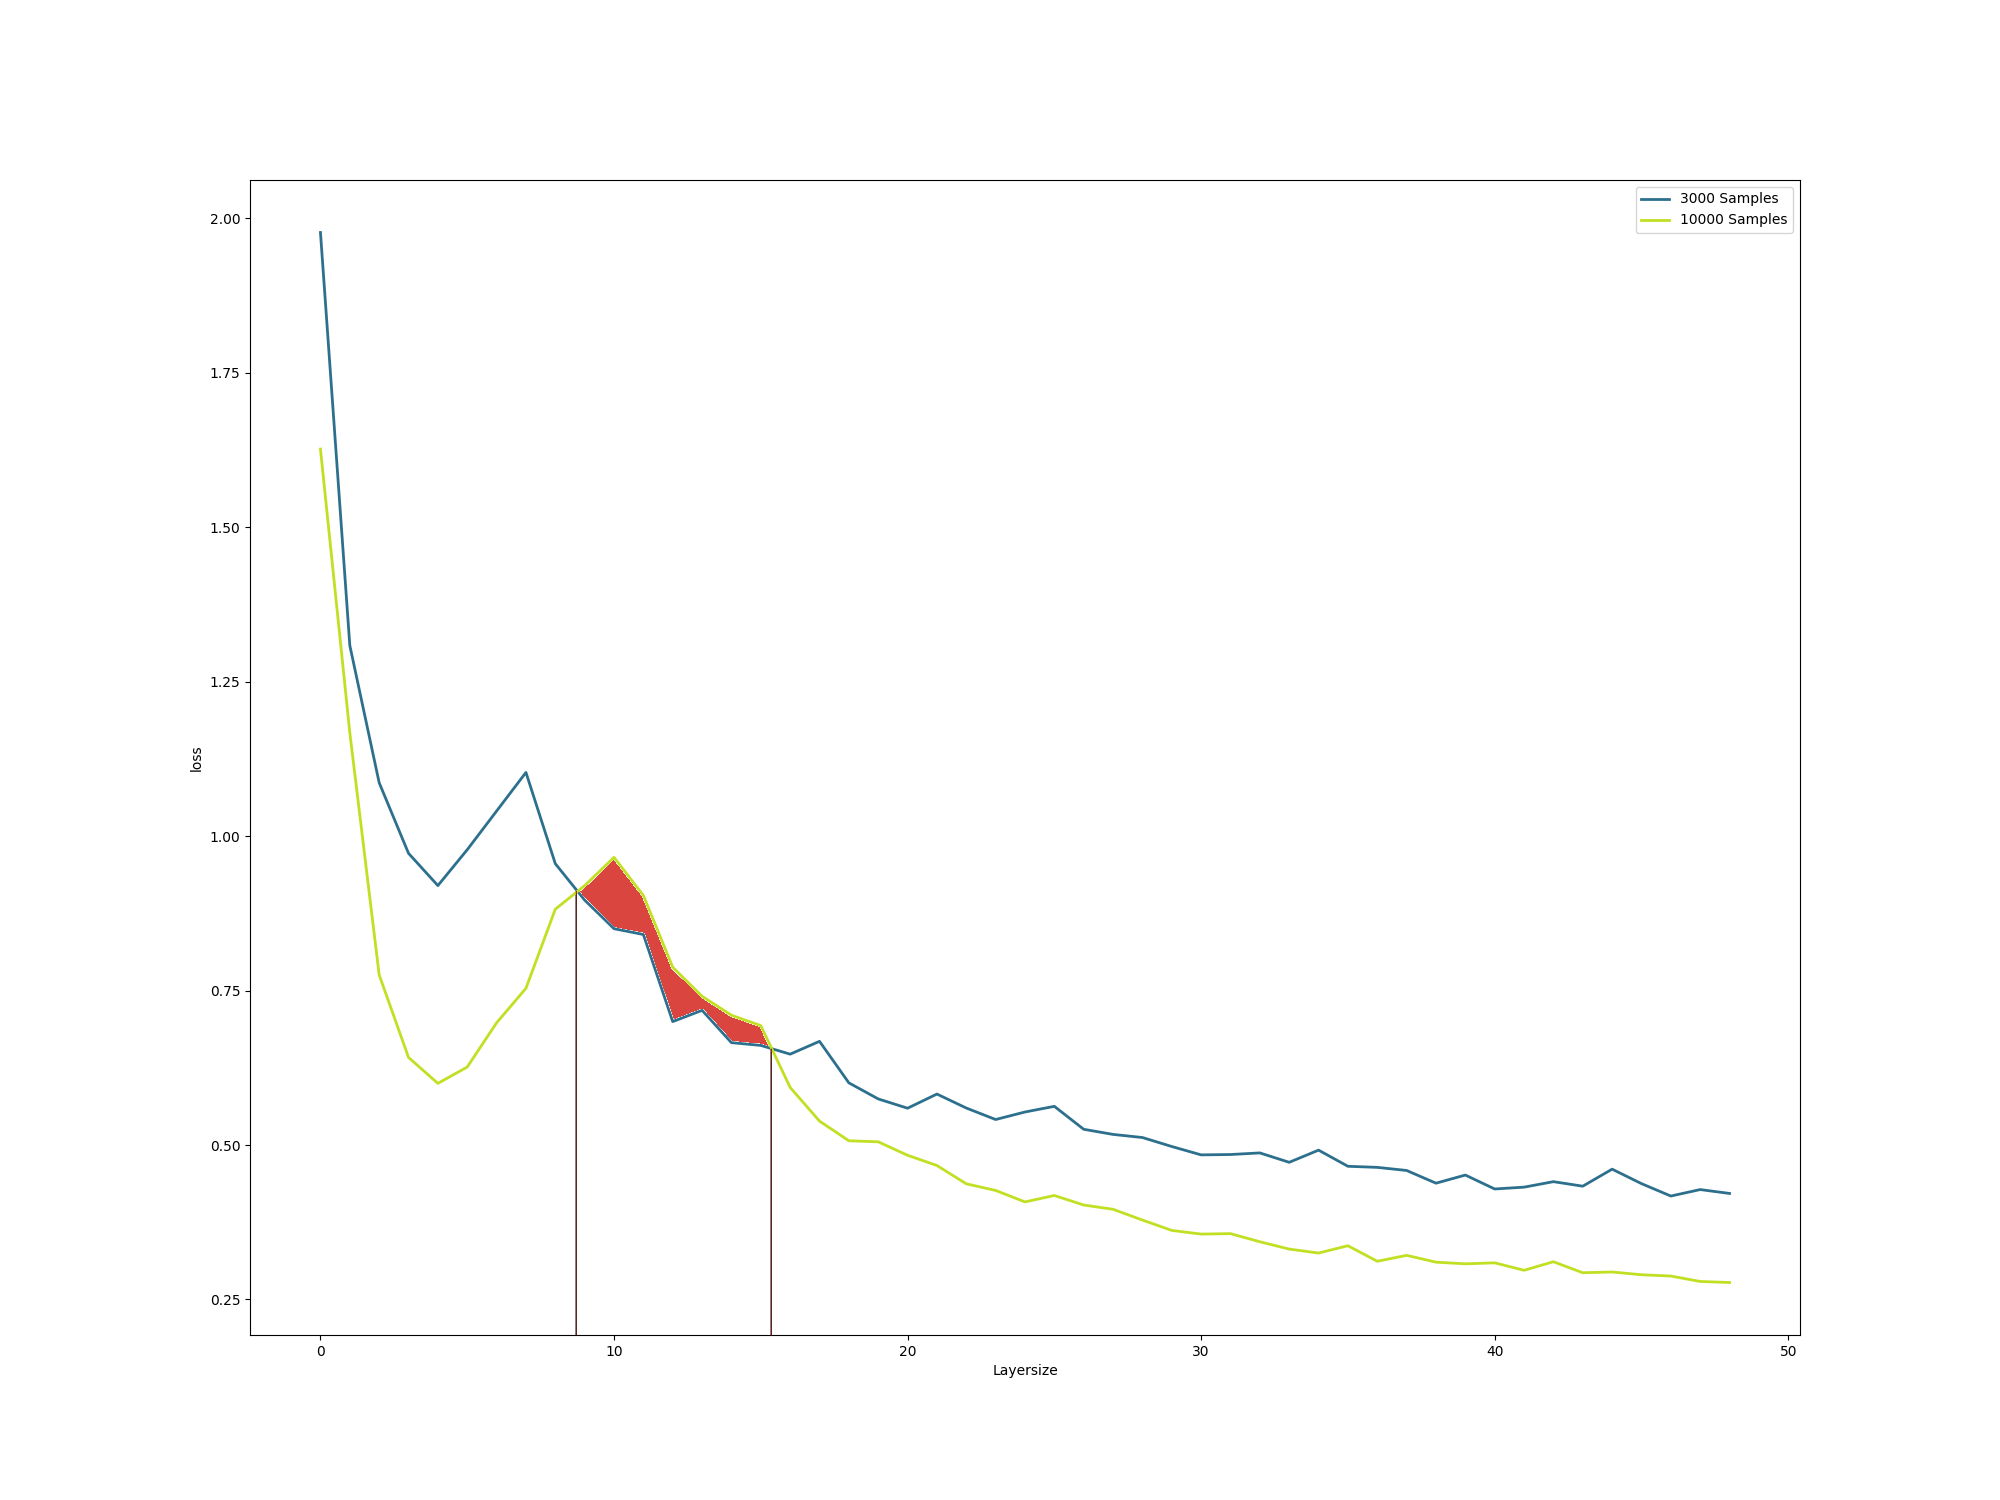
\includegraphics[width= 1\linewidth]{Abschlussarbeit_2021/LaTeX/images/more_is_less.png}
\caption{ Test loss with different sample size. Averaged over 8 runs. The red area indicates the modelsizes, where less data is better}
\label{fig:more_data_hurt}
\end{figure}
%%
%%%describtion ...


The result is shown in figure \ref{less_noise_can_hurt}. With a hidden layer size between $9 \leq H \leq 15$ the model trained with only 3000 samples performs better. 
%%

\subsection{Less noise can hurt}
\label{less_noise_can_hurt}
Another paradoxical phenomenon, which was already observed in chapter \ref{experimental_part}, is that at certain network sizes a higher proportion of noise in the labels can lead to better performance. Therefore, when choosing the model size, it should always be known which noise the data have. Wrong estimation can lead to worse generalization.

%%%
%%%
\begin{figure}[!htp]
\centering
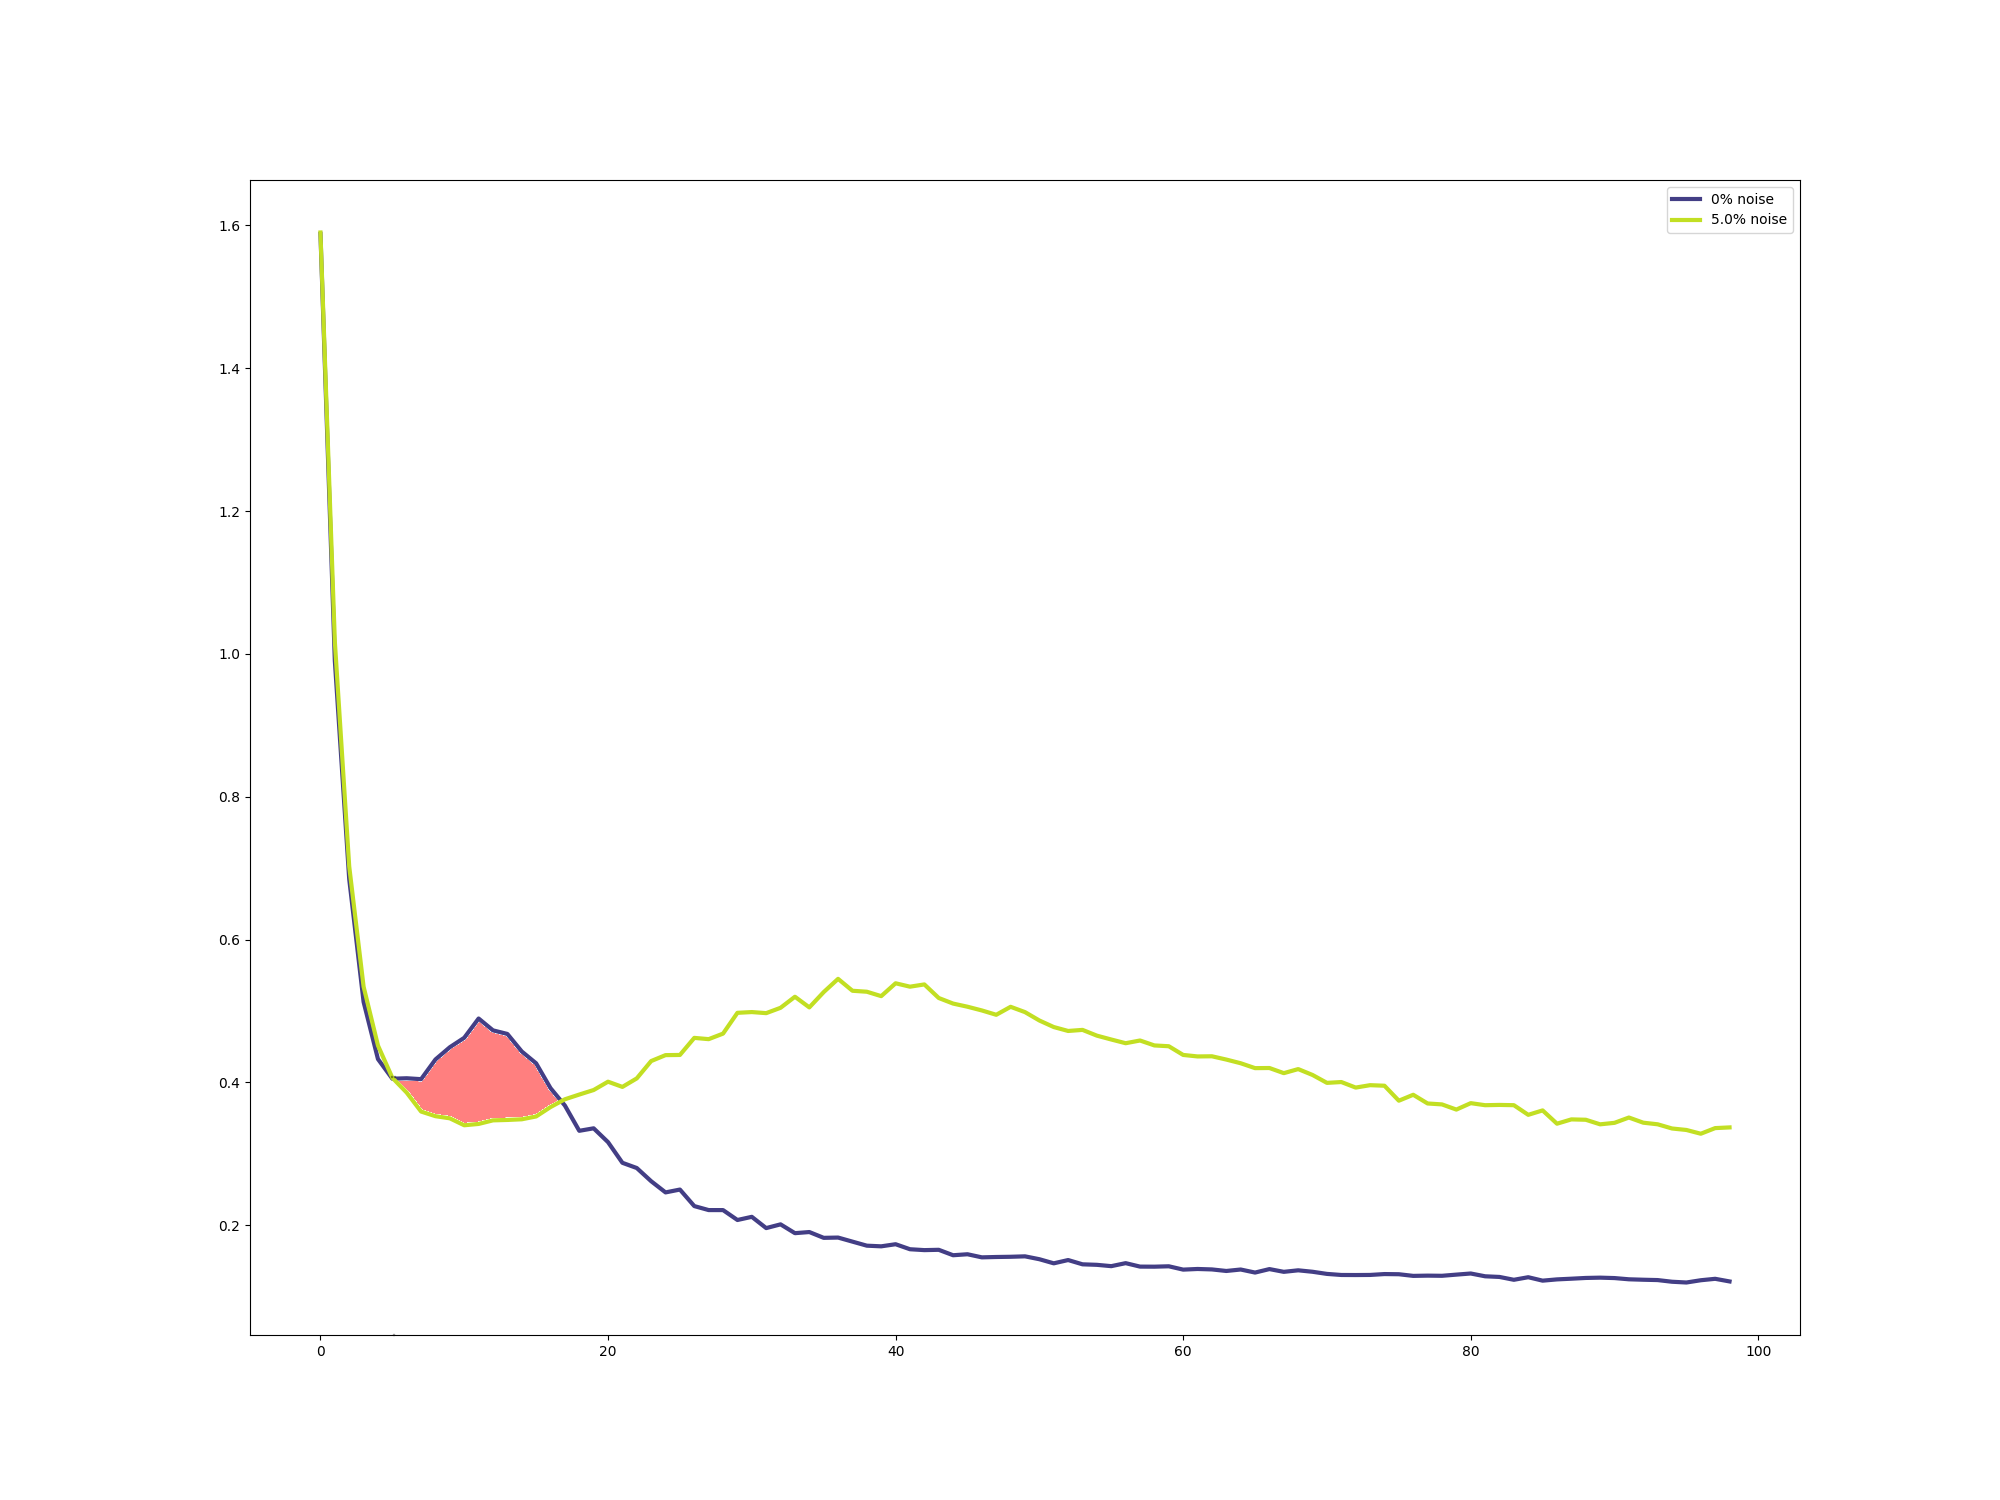
\includegraphics[width= 1\linewidth]{Abschlussarbeit_2021/LaTeX/images/more_noise_hurt.png}
\caption{ Test loss with different label noise. Averaged over 8 runs }
\label{more_noise_can_hurt}
\end{figure}
%%%%

This effect is due to overfitting. Due to the existing noise, it is only possible for networks to interpolate the data set with a high amount of parameters. With a lower amount of parameters the noise in the data set can act as a regularisation term because the Network is far away from interpolating the training data due to the noise. On the other hand, with low noise, overfitting is strong with the same amount of parameters because the interpolation threshold can here be reached much faster.

\subsection{Epoch-weise double descend}
In this thesis, Double Descent was demonstrated only in fully connected neural networks. However double descent can occur all types of neural networks like convolutional-neural-networks and ResNets \cite{Nakkiran_2021_more_data_hurt}. It it is even a phenomenon that occurs in other types of models as well. Double descent is also found in the Random-Forest regression procedure. This was also shown in \cite{belkin}.
However, for the constructed curves we have always changed the number of parameters of the network. Therefore, we can also speak of a parameter-wise double descent. However, there is an additional epoch-wise double descent. This was described for example in \cite{Nakkiran_2021_more_data_hurt}. So there is a similar curve behavior if the model size is fixed but changes the number of epochs. 

\begin{figure}[!htp]
\centering
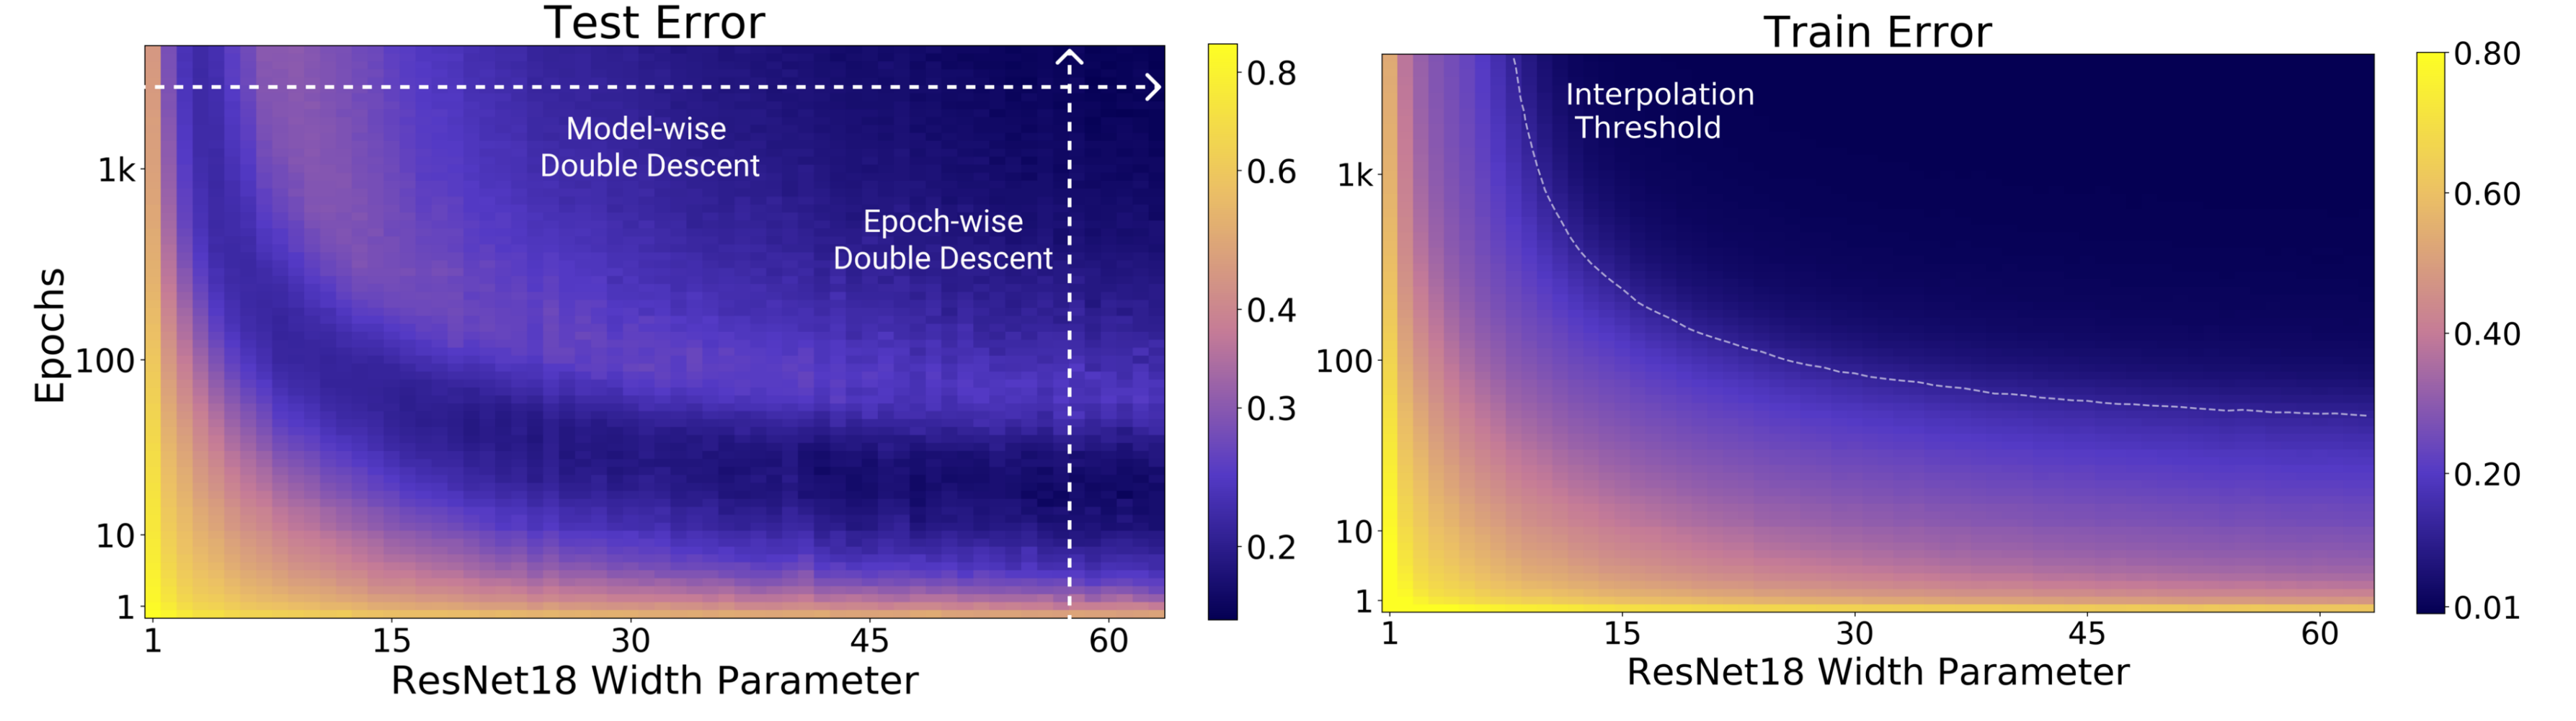
\includegraphics[width= 1\linewidth]{Abschlussarbeit_2021/LaTeX/images/Epochwise.PNG}
\caption{ Figures are taken from \cite{Nakkiran_2021_more_data_hurt}. On the left site the test error can be viewed and on the right side the train error can be seen. the $y$-axis indicates the amount of epochs and the $x$-axes describes the Network size.The convolutional network Resnet18s was trained on CIFAR-10 with 15\% label noise }
\label{fig: epochwise double descent}
\end{figure}

This can also be used under very specific circumstances. However, the epoch-wise double descent probably has less practical application to the training procedure than the parameter-wise variant. It is beyond the scope of this paper to investigate this in more detail. However, the fact that this phenomenon also occurs epoch-wise is highly interesting and is also being extensively researched. It should therefore be mentioned in any case. 







%%%
%%important in this chapter is also, that double descent can occur epochwiese and that double descent %%is even be found in decisiontrees and random forest etc
 
%%
%%larger models are simpler
%%

\newpage


\chapter{Conclusion}

In the first part of the work, the experimental part, the double Descent phenomena is first verified and then the influence of certain parameters and architectures is investigated. For a more detailed description, what kind of influence which parameter has, we refer to the discussion in chapter \ref{Discussion}.  However, it can be summarized that the phenomenon occurs under different optimization algorithms and network architectures. \\
 is the shape of the curve predictable? This question from the introduction can be answered with "yes". If the parameters are known, chapter \ref{experimental_part} shows that the resulting curve has certain predictable properties.\\ 
 In the second chapter, the behavior of the curve is analyzed in more detail. For this purpose, two sections of the double descent risk curve are examined individually. The two sections in question are called the underparameterized region and the overparameterized region. They are separated by the interpolation threshold, from which training data are completely interpolated. \\
A justification for the behavior of the curve in the underparameterized region is provided by the bias variance trade-off. It explains how the error term to be minimized depends on bias and variance. The dependence derived in the chapter (\ref{bias_variance_eq}) provides the shape of the first part of the curve. \\
For the second regime of the double descent risk curve, the overparameterized region, such a precise explanation for the behavior is missing. Nevertheless, assumptions can be made on the basis of observations on performed experiments. \\
The said observations occupy a large section of the thesis. First, learned functions are examined in dependence of the network size. It turns out that more parameters in models lead to a smoother learned function. larger neural networks have a feel for the distribution of the data and therefore generalize better.
It is also shown that average weight changes and epochs needed to find a minimum that ensures that the training data set is interpolated decreases with increasing parameter number. It can be observed that the decrease is proportional to the generalization curve, i.e. the test loss. It can therefore be assumed that larger networks find it much easier to interpolate the training data.\\
Another important finding is that the decomposition of the error from bias and variance (\ref{bias_variance_eq}) must also hold in the overparameterized domain. The conclusion from this is that the variance must fall monotonically in the overparameterized range. This is a finding which fits well with the observations just described. Thus, simpler and simpler functions can no longer vary so strongly. A smaller average weight change as well as a smaller number of required epochs also suggests that learned functions do not vary so much among themselves.\\
Following the observations made, two theories are presented as possible explanations for the monotonic decrease of the curve in the overparameterized region. The first theory states that larger networks have a self-regulatory influence on the training process. Thus, despite interpolation of the training data, weaker overfitting occurs. This theory is also consistent with the observations made. Thus, smaller weight changes and a lower variance have a regularizing influence.\\
The second theory is called the "winning lottery hypothesis". Here it is assumed that there are subgraphs in network graphs which allow a good convergence of SGD by their initialization. These subgraphs are called "winning tickets". A linear increase of the number of parameters causes an exponential increase of the number of subnetworks. The probability of a well initialized subnetwork thus increases. \\
The question from the beginning of the thesis, how the drop of the double descent curve can be explained, cannot be answered exactly. However, the idea why the test loss decreases with increasing number of parameters has become tangible after the thesis. It is also plausible why the performance does not increase after the interpolation threshold. This is due to the fact that data can be interpolated with different ellegance. \\
Chapter \ref{train_dd} shows interesting effects that can occur during training due to the double descent phenomenon. A seemingly paradoxical finding is that double descent can lead to poorer performance, for a given model size, with more data. Performance can be improved by taking into account double descent. \\

Chapter \ref{train_dd} has already shown us the importance of the double descent risk curve. But not only for reasons of better performance of the networks the phenomenon should be investigated further. It also gives us further understanding to a technique, the neural networks, whose behavior still cannot be completely explained. Especially with the more and more relevant topic of artificial intelligence in our everyday life. Exploring the functionality of neural networks is therefore an important aspect.
More and more papers dealing with this topic confirm this. The high number of published papers also shows how broad and versatile this topic is. Thus, this thesis could cite many more papers. But this would be beyond the scope of this work.  Even so, parts of this work were only superficially touched. For example, it would be interesting to further investigate the loss landscape of overparameterized networks, since the use of the SAM optimizer has produced an interesting generalization curve. \\
Proving the lottery ticket hypothesis would also be an interesting topic for further work. After all, this hypothesis has already yielded astonishing results. \\
It would also be interesting to know how many minimums exist depending on the number of parameters that interpolate the training data. Thus, further insights into the self regularizing effect of larger networks could be gained. \\
So there is still much to speculate on the subject of double descent and it can be eagerly awaited what knowledge will be gained about it in the future.









%\chapter{Conclusion}

In the first part of the work, the experimental part, the double Descent phenomena is first verified and then the influence of certain parameters and architectures is investigated. For a more detailed description, what kind of influence which parameter has, we refer to the discussion in chapter \ref{Discussion}.  However, it can be summarized that the phenomenon occurs under different optimization algorithms and network architectures. \\
 is the shape of the curve predictable? This question from the introduction can be answered with "yes". If the parameters are known, chapter \ref{experimental_part} shows that the resulting curve has certain predictable properties.\\ 
 In the second chapter, the behavior of the curve is analyzed in more detail. For this purpose, two sections of the double descent risk curve are examined individually. The two sections in question are called the underparameterized region and the overparameterized region. They are separated by the interpolation threshold, from which training data are completely interpolated. \\
A justification for the behavior of the curve in the underparameterized region is provided by the bias variance trade-off. It explains how the error term to be minimized depends on bias and variance. The dependence derived in the chapter (\ref{bias_variance_eq}) provides the shape of the first part of the curve. \\
For the second regime of the double descent risk curve, the overparameterized region, such a precise explanation for the behavior is missing. Nevertheless, assumptions can be made on the basis of observations on performed experiments. \\
The said observations occupy a large section of the thesis. First, learned functions are examined in dependence of the network size. It turns out that more parameters in models lead to a smoother learned function. larger neural networks have a feel for the distribution of the data and therefore generalize better.
It is also shown that average weight changes and epochs needed to find a minimum that ensures that the training data set is interpolated decreases with increasing parameter number. It can be observed that the decrease is proportional to the generalization curve, i.e. the test loss. It can therefore be assumed that larger networks find it much easier to interpolate the training data.\\
Another important finding is that the decomposition of the error from bias and variance (\ref{bias_variance_eq}) must also hold in the overparameterized domain. The conclusion from this is that the variance must fall monotonically in the overparameterized range. This is a finding which fits well with the observations just described. Thus, simpler and simpler functions can no longer vary so strongly. A smaller average weight change as well as a smaller number of required epochs also suggests that learned functions do not vary so much among themselves.\\
Following the observations made, two theories are presented as possible explanations for the monotonic decrease of the curve in the overparameterized region. The first theory states that larger networks have a self-regulatory influence on the training process. Thus, despite interpolation of the training data, weaker overfitting occurs. This theory is also consistent with the observations made. Thus, smaller weight changes and a lower variance have a regularizing influence.\\
The second theory is called the "winning lottery hypothesis". Here it is assumed that there are subgraphs in network graphs which allow a good convergence of SGD by their initialization. These subgraphs are called "winning tickets". A linear increase of the number of parameters causes an exponential increase of the number of subnetworks. The probability of a well initialized subnetwork thus increases. \\
The question from the beginning of the thesis, how the drop of the double descent curve can be explained, cannot be answered exactly. However, the idea why the test loss decreases with increasing number of parameters has become tangible after the thesis. It is also plausible why the performance does not increase after the interpolation threshold. This is due to the fact that data can be interpolated with different ellegance. \\
Chapter \ref{train_dd} shows interesting effects that can occur during training due to the double descent phenomenon. A seemingly paradoxical finding is that double descent can lead to poorer performance, for a given model size, with more data. Performance can be improved by taking into account double descent. \\

Chapter \ref{train_dd} has already shown us the importance of the double descent risk curve. But not only for reasons of better performance of the networks the phenomenon should be investigated further. It also gives us further understanding to a technique, the neural networks, whose behavior still cannot be completely explained. Especially with the more and more relevant topic of artificial intelligence in our everyday life. Exploring the functionality of neural networks is therefore an important aspect.
More and more papers dealing with this topic confirm this. The high number of published papers also shows how broad and versatile this topic is. Thus, this thesis could cite many more papers. But this would be beyond the scope of this work.  Even so, parts of this work were only superficially touched. For example, it would be interesting to further investigate the loss landscape of overparameterized networks, since the use of the SAM optimizer has produced an interesting generalization curve. \\
Proving the lottery ticket hypothesis would also be an interesting topic for further work. After all, this hypothesis has already yielded astonishing results. \\
It would also be interesting to know how many minimums exist depending on the number of parameters that interpolate the training data. Thus, further insights into the self regularizing effect of larger networks could be gained. \\
So there is still much to speculate on the subject of double descent and it can be eagerly awaited what knowledge will be gained about it in the future.









%\appendix
% hier Anhänge einbinden

%%TODO
\appendix

\chapter{Apendix}

\section{Experimental part }

Refered to the Chapter \ref{experimental_part}. A few more interesting plots will be presented.\\
The Code for the experiments was written in Python with help from the \hyperlink{https://www.tensorflow.org/resources/libraries-extensions}{TensorFlow} extension.\\
The code for the experiments can be found on \hyperlink{https://github.com/RitterRost/Bachelorarbeit.git}{github}\footnote{\url{https://github.com/RitterRost/Bachelorarbeit.git}}

\begin{figure}[!htp]
\centering
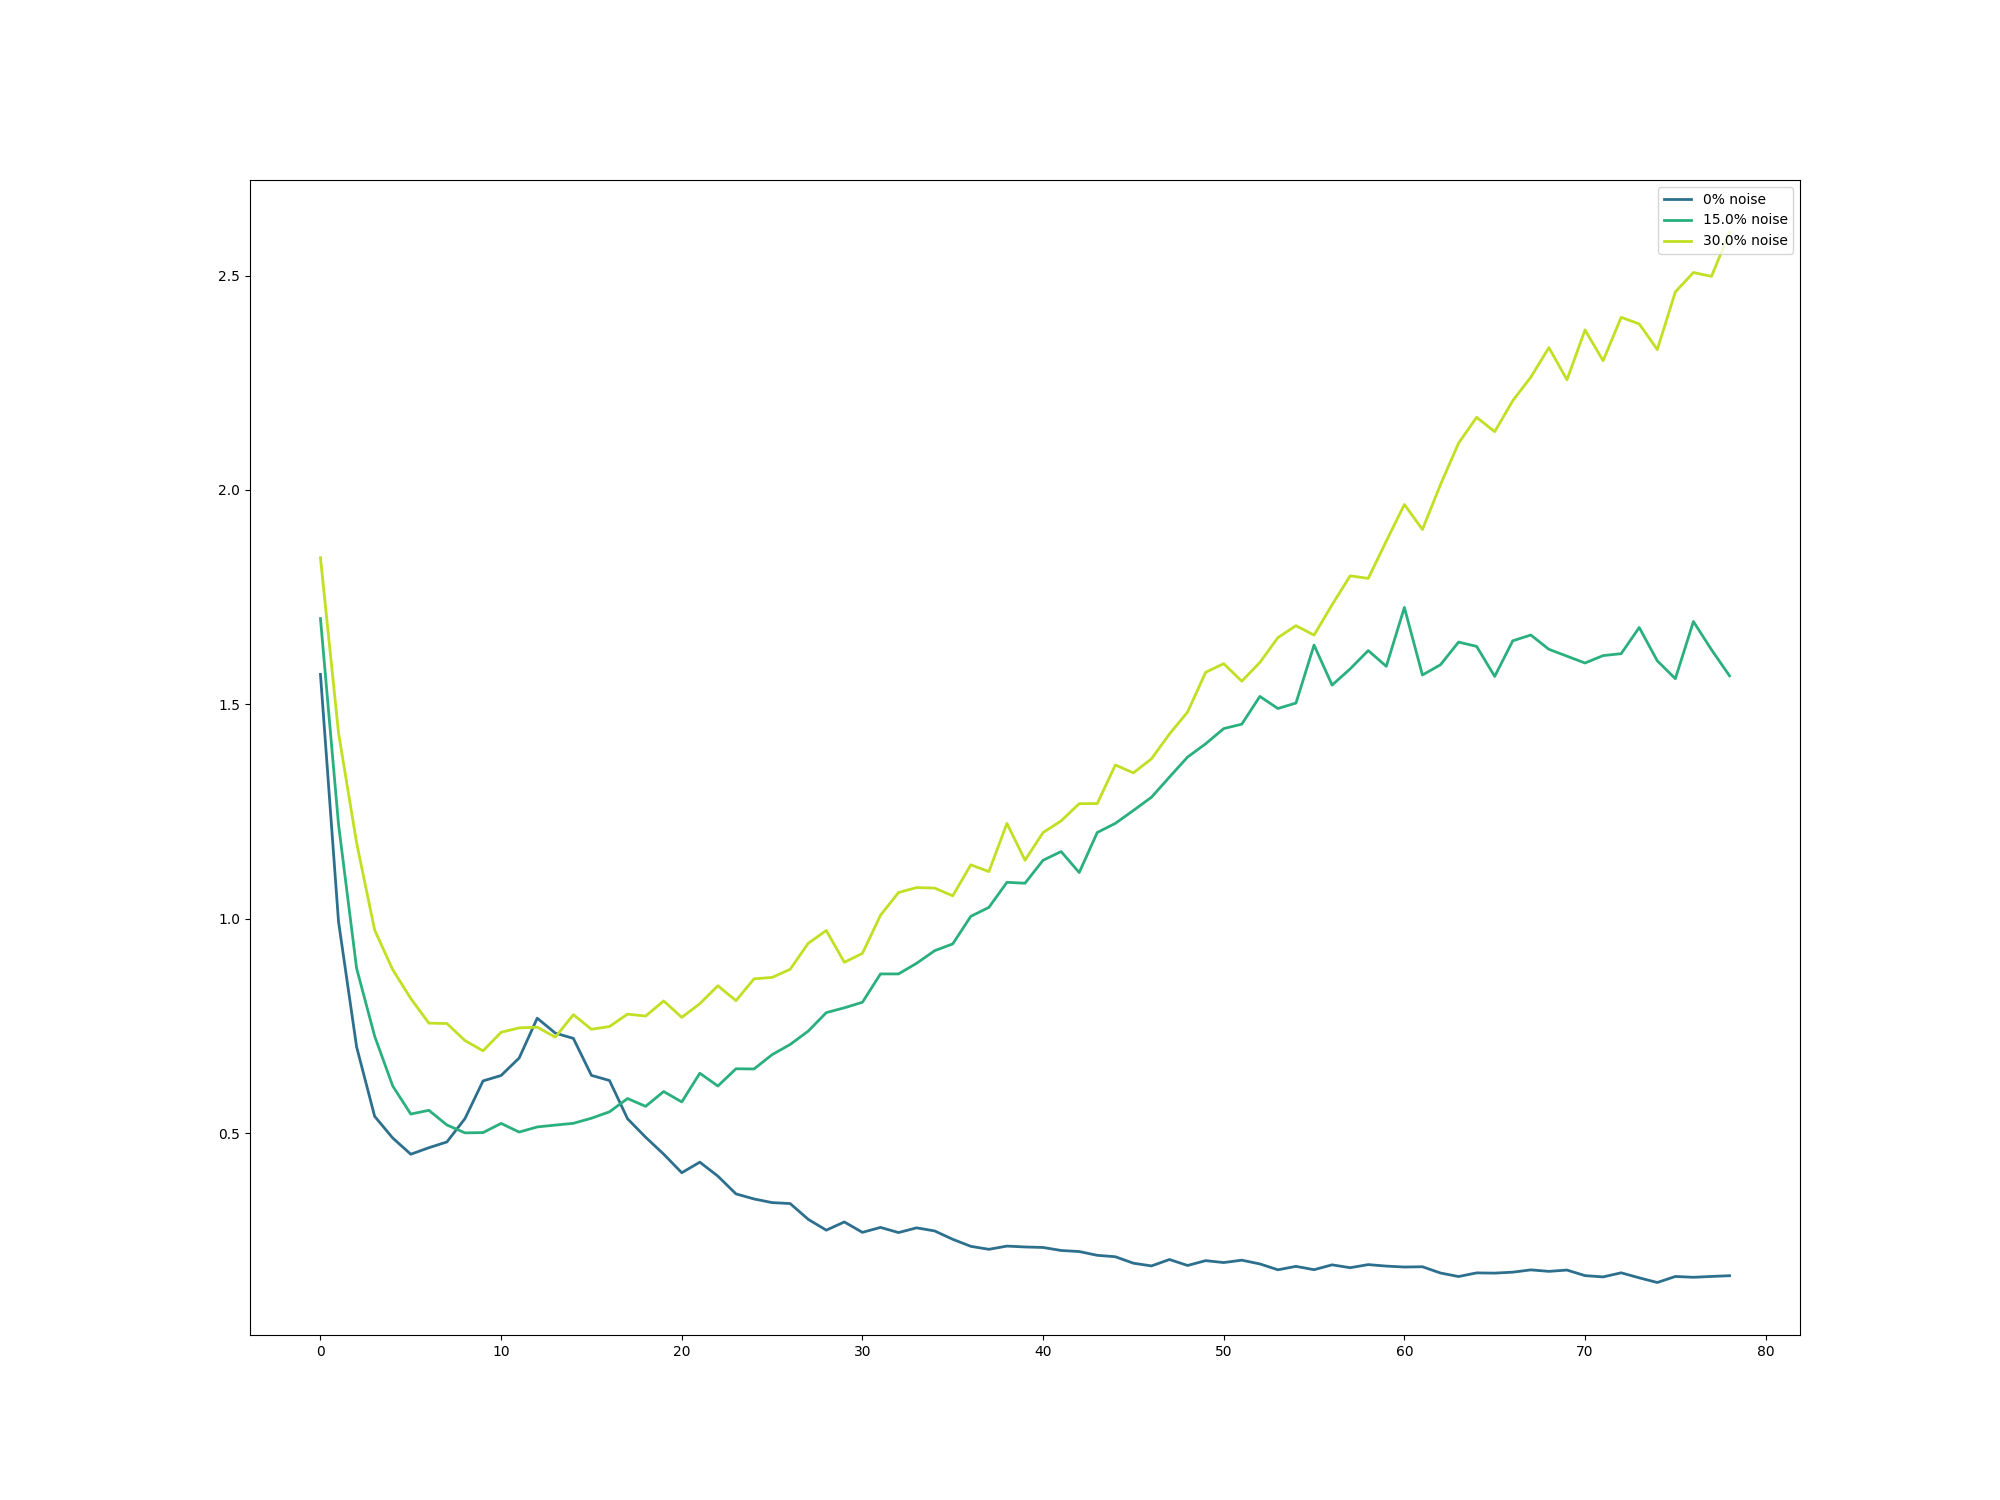
\includegraphics[width= 0.8\linewidth]{Abschlussarbeit_2021/LaTeX/images/noisy_curve.png}
\caption{this graph shows what happens when the noise level is set extremely high. It can be guessed that Double Descent occurs anyway, even if the interpolation threshold occurs only at large layer size $H$. This graph is a supplement to figure \ref{fig:Label_noise_on_double_descent}.}
\label{more_noise_can_hurt}
\end{figure}

\begin{figure}[!htp]
\centering
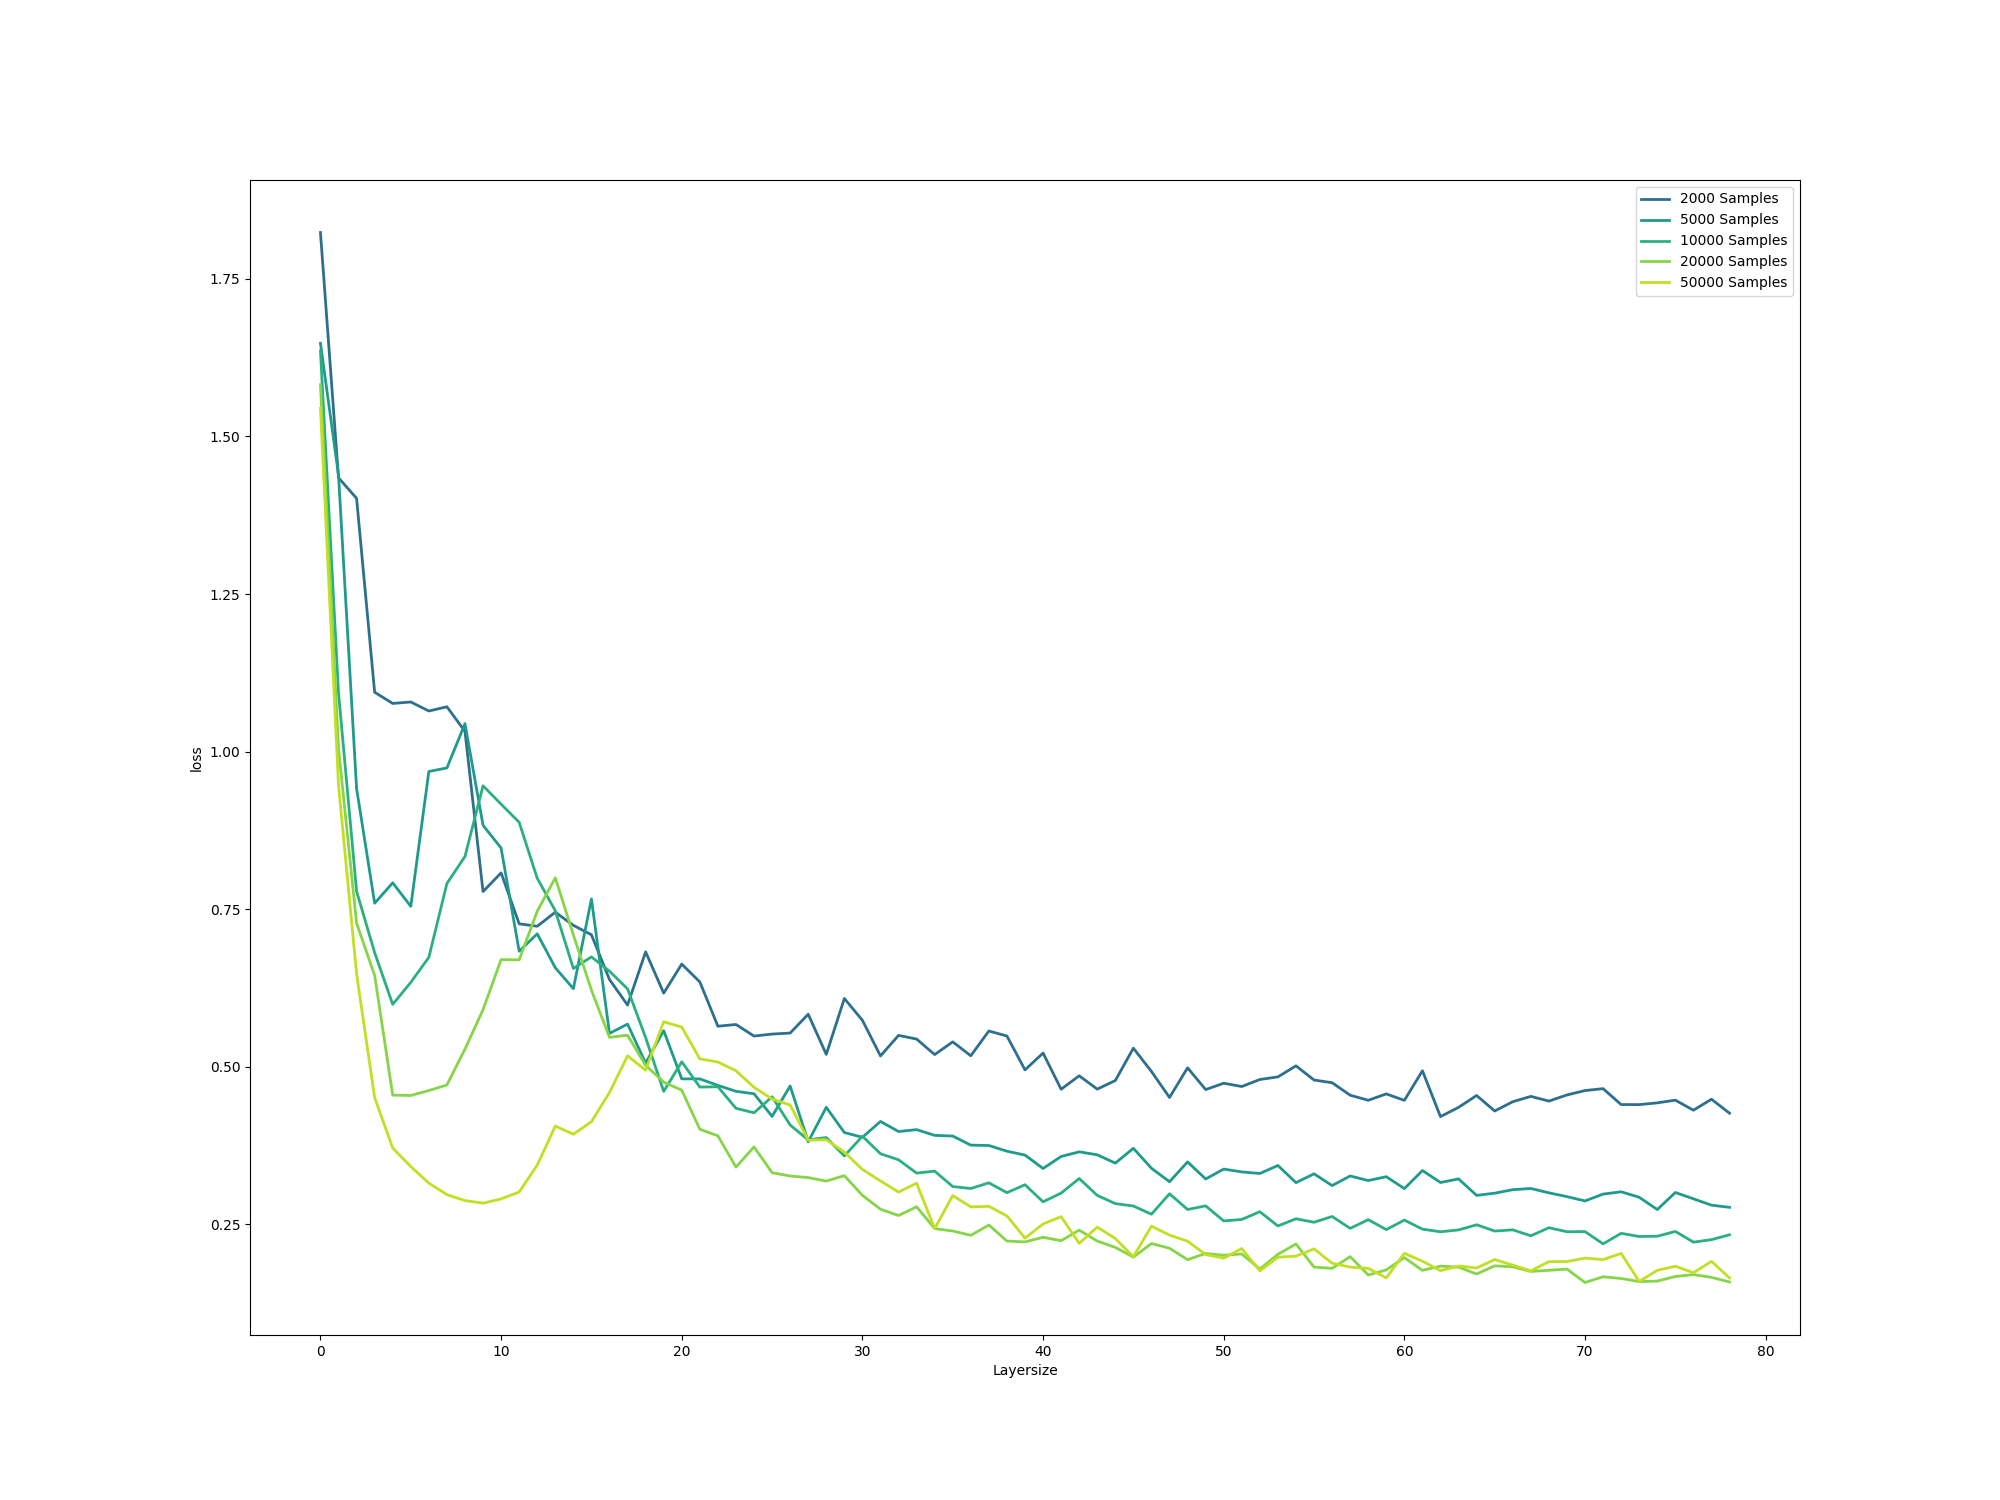
\includegraphics[width= 0.8\linewidth]{Abschlussarbeit_2021/LaTeX/images/many_samplesizes.png}
\caption{This graphic refers to figure \ref{fig:sample_size_double_descent}. Different sample sizes have been added as well. The described effect in \ref{more_noise_can_hurt} can also be observed here.}
\label{more_noise_can_hurt}
\end{figure}


\section{Investigations and possible Explanations for the behavior of the curve}

\subsection{Bias variance trade-off}
\label{bv_help_eq}
We want to show that $E[X^2] = Var[X] + E[X]^2$. \\
This directly follows out of 
$$
Var(X) = E[(X-E[x])^2] = E[X^2] + E[X]^2 - 2E[X\cdot E[x]]
$$
$$
\Longleftrightarrow Var(X) = E[X^2] + E[X]^2 - 2E[X]^2 = E[X^2] - E[X]^2 
$$
$$
\Longleftrightarrow E[X^2] = Var[X] + E[X]^2
$$
This Equation is also known as the displacement theorem from Steiner.

\subsection{Experiments on RFFs}

\subsubsection{Proof for the optimal function in experiment \ref{fig:1d_rff}}
\label{proof_for_1d_rff}
Let $D \in \mathbb{R}^{n \times 2}$ be the generated data points. 
To minimize the Error we have to minimize the term,
$$
\sum_{(x,y) \in D} E[(y - f(x))^2] = \sum_{(x,y) \in D} E[(y)^2] - 2\cdot E[y]\cdot E[f(x)] +  E[f(x)^2]
$$
$$
\Longleftrightarrow \sum_{(x,y) \in D} E[(y - f(x))^2] = \sum_{(x,y) \in D} E[y^2 + f(x)^2] - 2\cdot E[y]\cdot E[f(x)] 
$$
We know that $E[(y - f(x))^2] \geq 0$ and is therefore minimal if $E[(y - f(x))^2] = 0$
$$
\Rightarrow \sum_{(x,y) \in D} E[y^2 + f(x)^2] = \sum_{(x,y) \in D} 2\cdot E[y]\cdot E[f(x)]  
$$
This holds if $E[y] = E[f(x)]$  $\forall (x,y) \in D$. $E[y] = m \cdot x + c$ is given by definition. Therefore,   
$$
f(x) = m\cdot x + c 
$$
is a best possible solution for the problem. And it is also the only global minima because $E[y^2 + f(x)^2] \geq 0$.


\subsubsection{Proof for the optimal function in experiment \ref{3d_RFF}}
Here the same argument as in \ref{proof_for_1d_rff} holds.
Let $D \in \mathbb{R}^{n \times 3}$ be the generated data points. 
To minimize the Error we have to minimize the term,
$$
\sum_{(x,y) \in D} E[(y - f(x))^2] = \sum_{(x,y) \in D} E[(y)^2] - 2\cdot E[y]\cdot E[f(x)] +  E[f(x)^2]
$$
We again use that $E[(y - f(x))^2] \geq 0$ and is therefore minimal if $E[(y - f(x))^2] = 0$
$$
\Rightarrow \sum_{(x,y) \in D} E[y^2] + E[f(x)^2] = \sum_{(x,y) \in D} 2\cdot E[y]\cdot E[f(x)]  
$$
$E[y] = 0$ $\forall (x,y) \in D$ is given by definition. 
$$
\Longleftrightarrow \sum_{(x,y) \in D} E[f(x)^2] = 0
$$
Because $f(x)^2 \geq 0$. The only best possible solution is given by the $x$-$y$-plane,
$$
f(x) = 0 
$$



\newpage

\subsubsection{Extrapolation in the experiment \ref{3d_RFF}}
\label{extrapolation}

It can be observed that models with more parameters perform better even with extrapolation. The successful extrapolation can also be due to the periodic properties of the fourier features.


\begin{figure}[!htp]
\centering
\begin{subfigure}{}
  \centering
  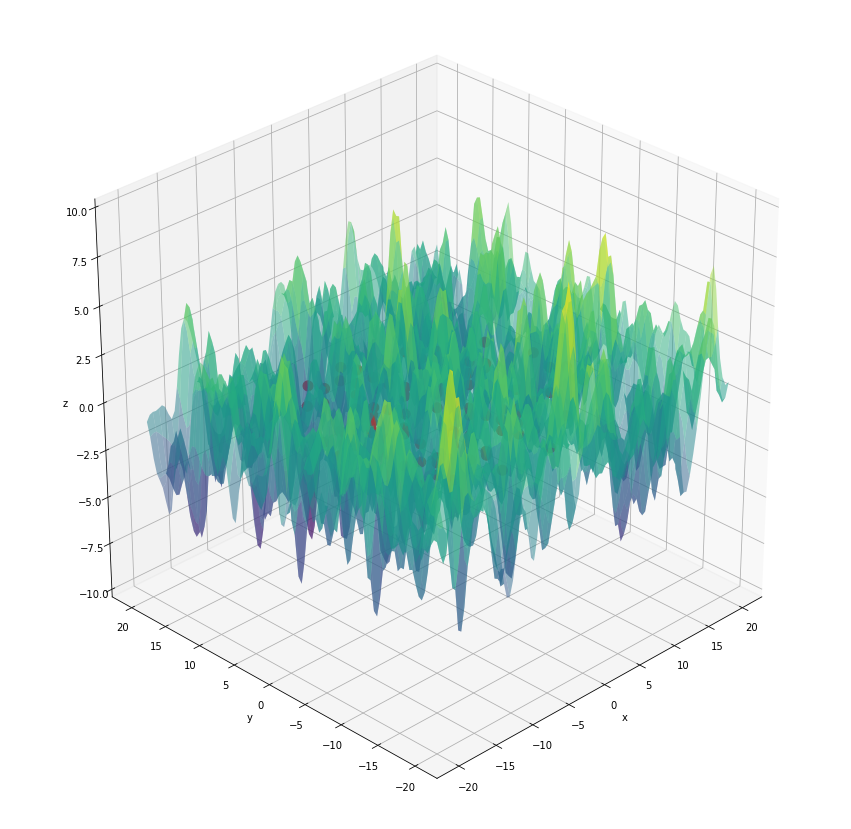
\includegraphics[width=.49\linewidth]{Abschlussarbeit_2021/LaTeX/images/extrapol_less.png}
  \label{fig:sub1}
\end{subfigure}%
\begin{subfigure}{}
  \centering
  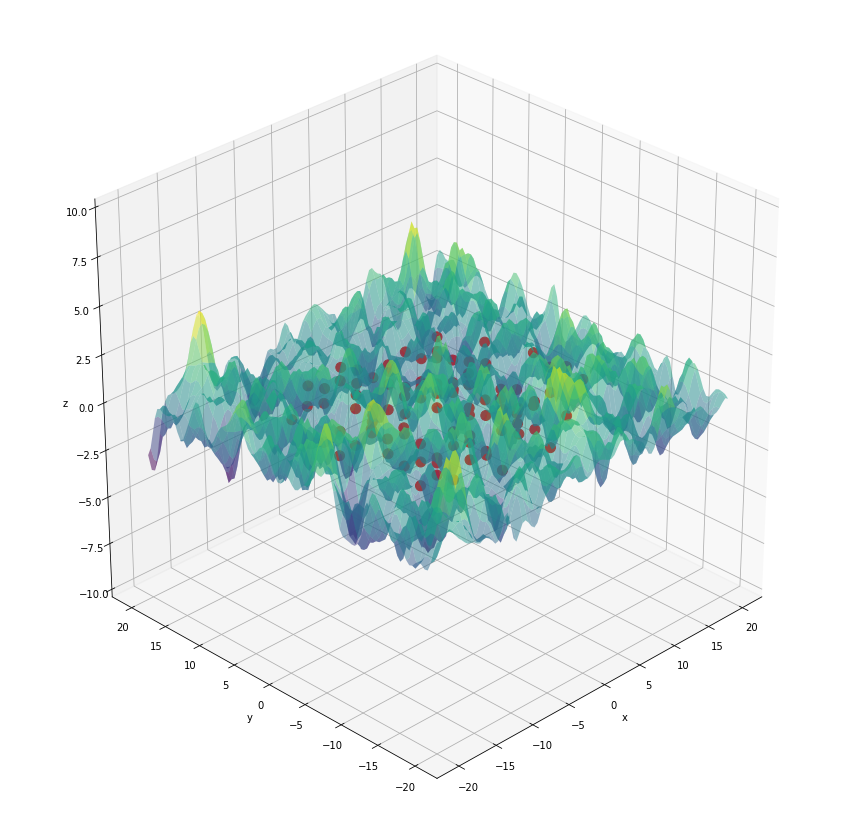
\includegraphics[width=.49\linewidth]{Abschlussarbeit_2021/LaTeX/images/extrapol_many.png}
  \label{fig:sub2}
\label{fig:high_varianz_with_noise}  
\end{subfigure}
\caption{The left plot shows a function learned from a model with $N = 120$ random fourier features. The right plot shows the function learned by a model with $N = 10000$ features. The red points are the data-points. The definition range in which the function is to be predicted is in this example larger as in \ref{3d_RFF} $([-20,20] \times [-20,20])$.}
\label{3d_RFF_extra}
\end{figure}

\subsection{Other interesting discoveries }

\subsubsection{Further plots to the SAM-optimizer }
\label{sam_extension}

In this section it can be observed what happens when the factor $\rho$ is increased in the SAM-optimizer. As mentioned in \ref{fig:sam} the test loss decreases at the interpolation threshold.

\begin{figure}[!htp]
\centering
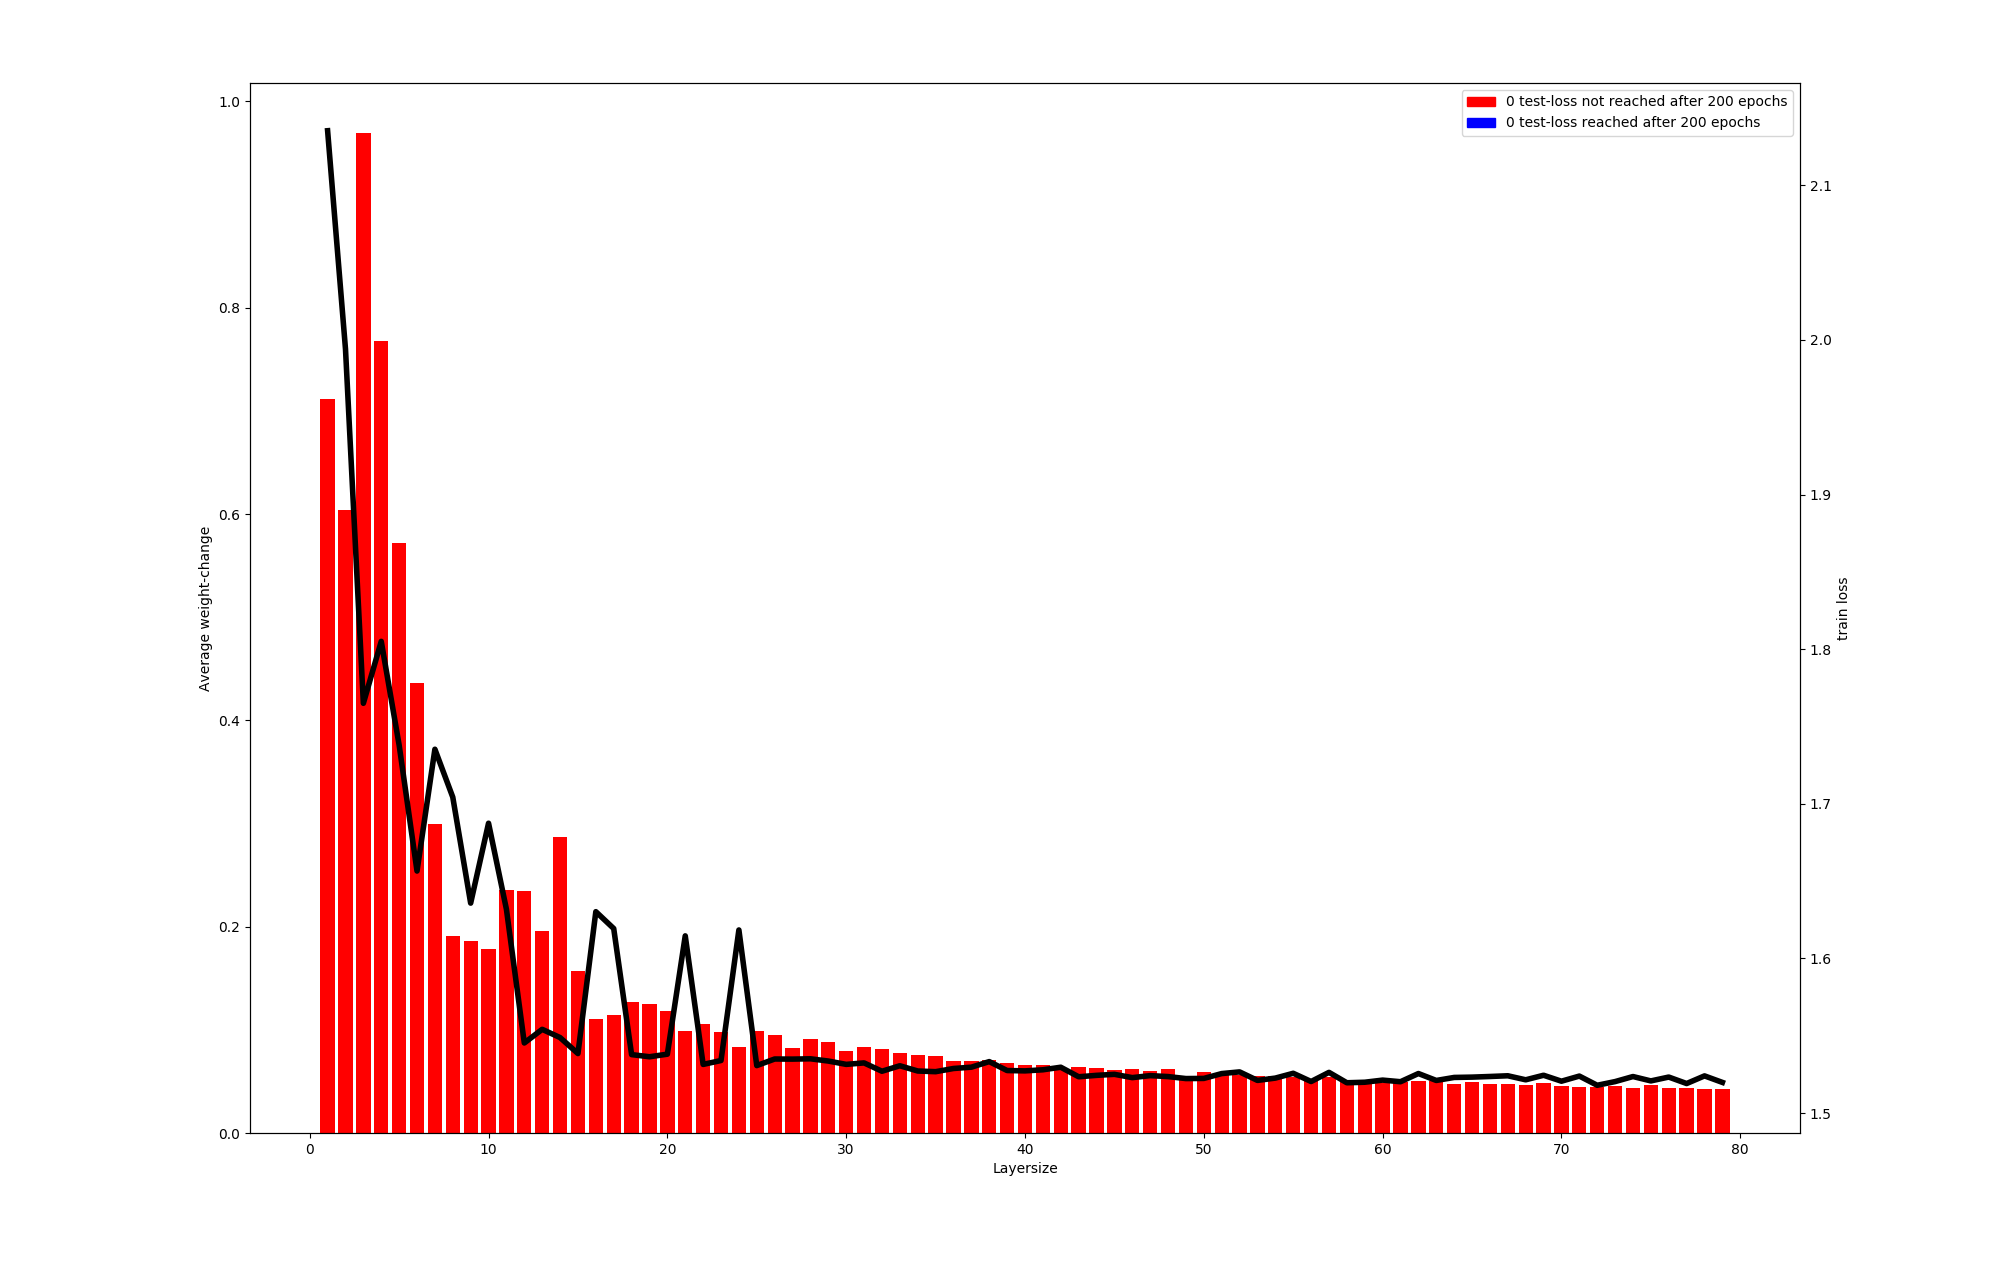
\includegraphics[width= 0.8\linewidth]{Abschlussarbeit_2021/LaTeX/images/sam_weigthchange.png}
\caption{A smoothing factor of $\rho = 0.1$
was used. The data set is a subset of MNIST with 15000 samples}
\label{more_noise_can_hurt}
\end{figure}

\begin{figure}[!htp]
\centering
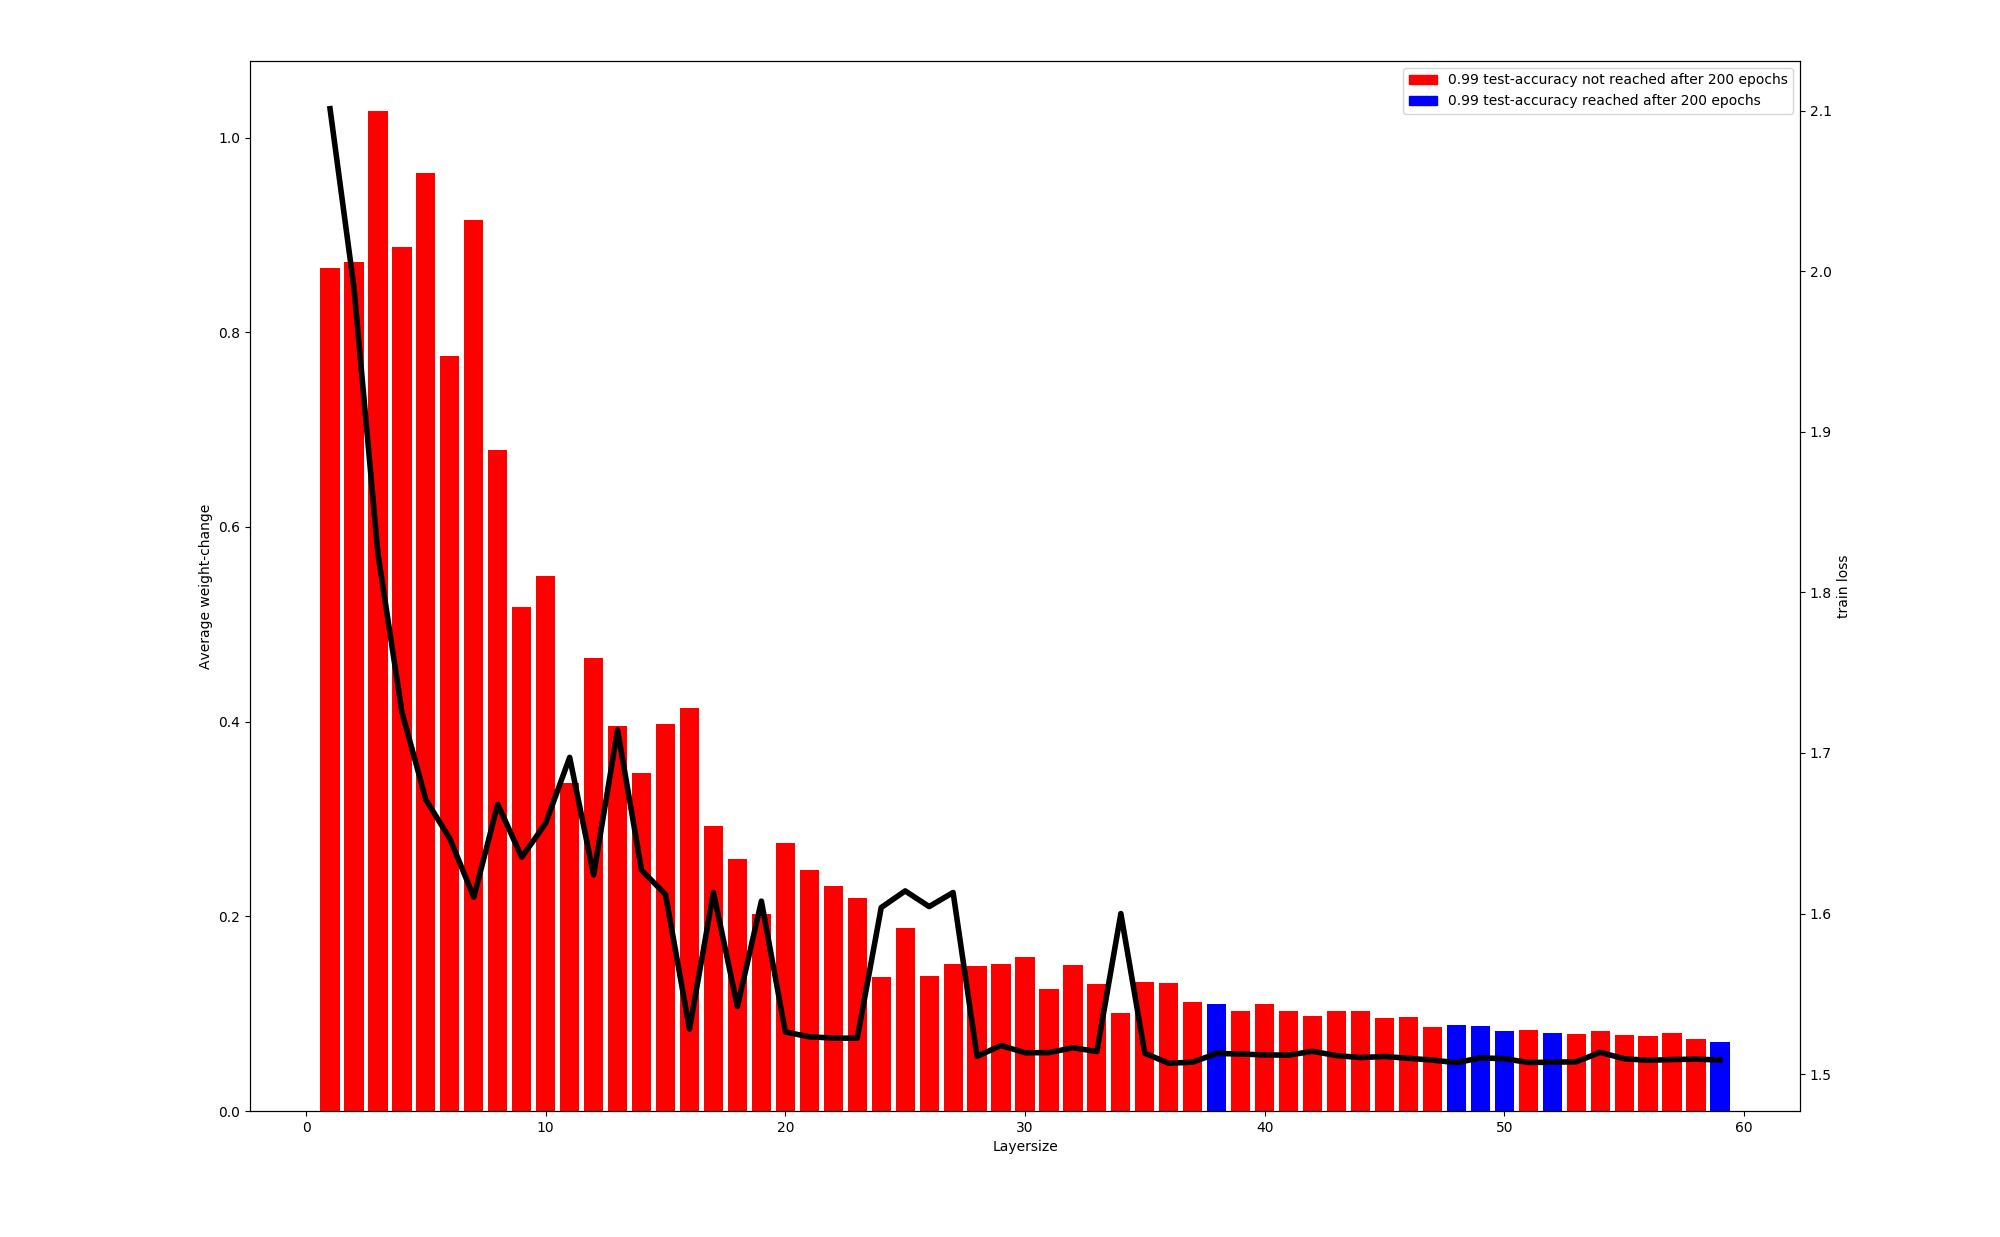
\includegraphics[width= 0.8\linewidth]{Abschlussarbeit_2021/LaTeX/images/sam_loss4_.png}
\caption{A smoothing factor of $\rho = 0.07$
was used. The data set is a subset of MNIST with 15000 samples}
\label{more_noise_can_hurt}
\end{figure}




















\backmatter

\nocite{belkin}
\nocite{pmlr-v97-brutzkus19b}
\nocite{pmlr-v119-d-ascoli20a}
\nocite{bias_variance_op}
\nocite{Nakkiran_2021_more_data_hurt}
\nocite{l2_regularization_double_descent}
\nocite{A_least_squre_study}
\nocite{prehistory_double_descent}
\nocite{lottery_ticket}
\nocite{weak_features_belkin}
\nocite{sam_optimizer}
\nocite{sharp_loss}
\nocite{dd_analysis}
\nocite{RF-model}
\nocite{Bergman}

%%websites
\nocite{romero_2021_tw_ds}
\nocite{double_descent_2021_splines}
\nocite{wikipedia_Mnist-Datenbank}
\nocite{wikipedia_Machine_learning}
\nocite{wikipedia_bias_variance}
\nocite{Artificial_neural_network}
\nocite{understanding_double_ticket}
\nocite{wikipedia_inductiv_bias}
\nocite{wine}
\nocite{regularization_L1_L2}



\setquotestyle{english}
\printbibliography

\clearpage
\thispagestyle{empty}

Name: \fullname \hfill Matrikelnummer: \matnr \vspace{2cm}

\minisec{Erklärung}

Ich erkläre, dass ich die Arbeit selbständig verfasst und keine anderen als die angegebenen Quellen und Hilfsmittel verwendet habe.\vspace{2cm}

Ulm, den \dotfill

\hspace{10cm} {\footnotesize \fullname}
\end{document}
